\documentclass[a4paper ]{article}
\usepackage{graphicx}
\usepackage[letterpaper, landscape, margin=2in]{geometry}
\geometry{
	paper=a4paper, % Change to letterpaper for US letter
	inner=0.5cm, % Inner margin
	outer=0.5cm, % Outer margin
	bindingoffset=0.01cm, % Binding offset
	top=0.5cm, % Top margin
	bottom=0.5cm, % Bottom margin
	%showframe, % Uncomment to show how the type block is set on the page
}
\usepackage[utf8]{inputenc}
%\usepackage{natbib}

\begin{document}
- - -

\vspace{50mm}
\begin{center}
{\Huge \textsc{\textbf{Exploración visual de datos individuales}}}\\
\vspace{20mm}
\end{center}

\begin{center}
\textit{\huge Estudios en Detección de Señales - Tesis de Licenciatura}\\
\bigskip
\end{center}

\begin{center}
\textit{\huge Adriana F. Chávez De la Peña}\\
\end{center}

\begin{center}
\vfill
\textit{\huge adrifelcha@gmail.com}\\
\end{center}

\newpage




---
\vspace{3mm}
\begin{center}
{\LARGE \textbf{Respuestas a la tarea 'Sí/No' registradas en cada ensayo}}\\
{\small \textsc{(para comprobar que todas las opciones de respuesta se hayan utilizado)}}\\
\smallskip
\end{center}
\begin{center}
{\LARGE \textit{Experimento 1}}\\
\end{center}

\vspace{3mm}
\begin{figure}[th]
\centering
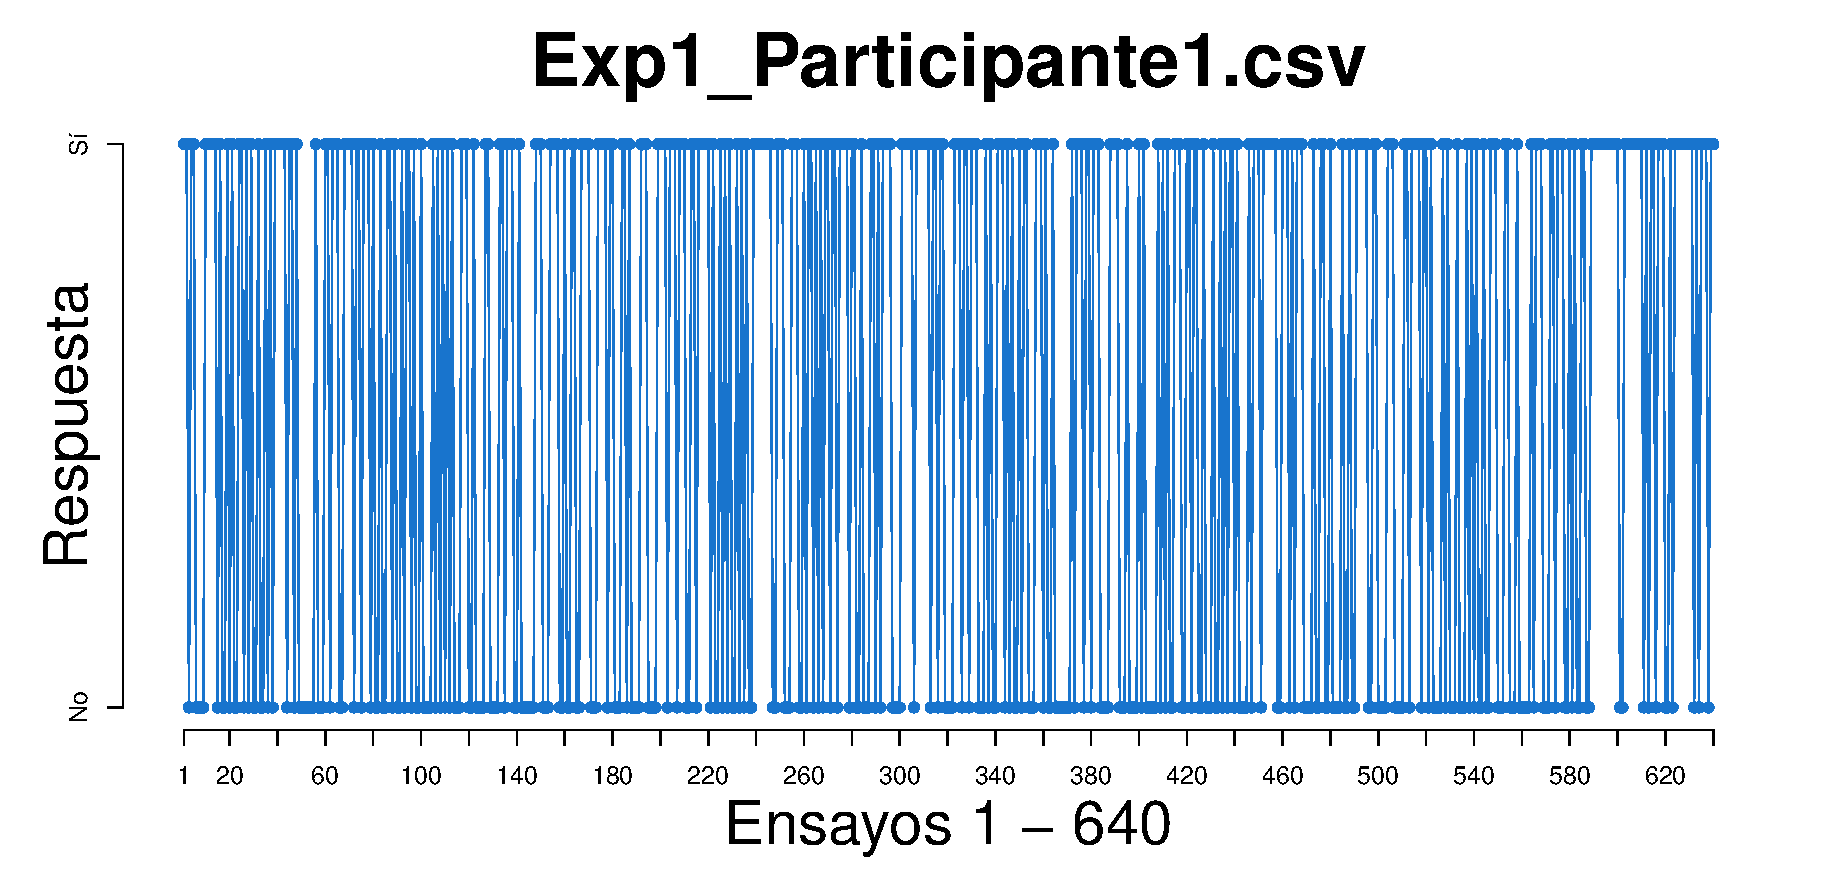
\includegraphics[width=9cm, height=5cm]{Figures/Response_Exp1_P1} 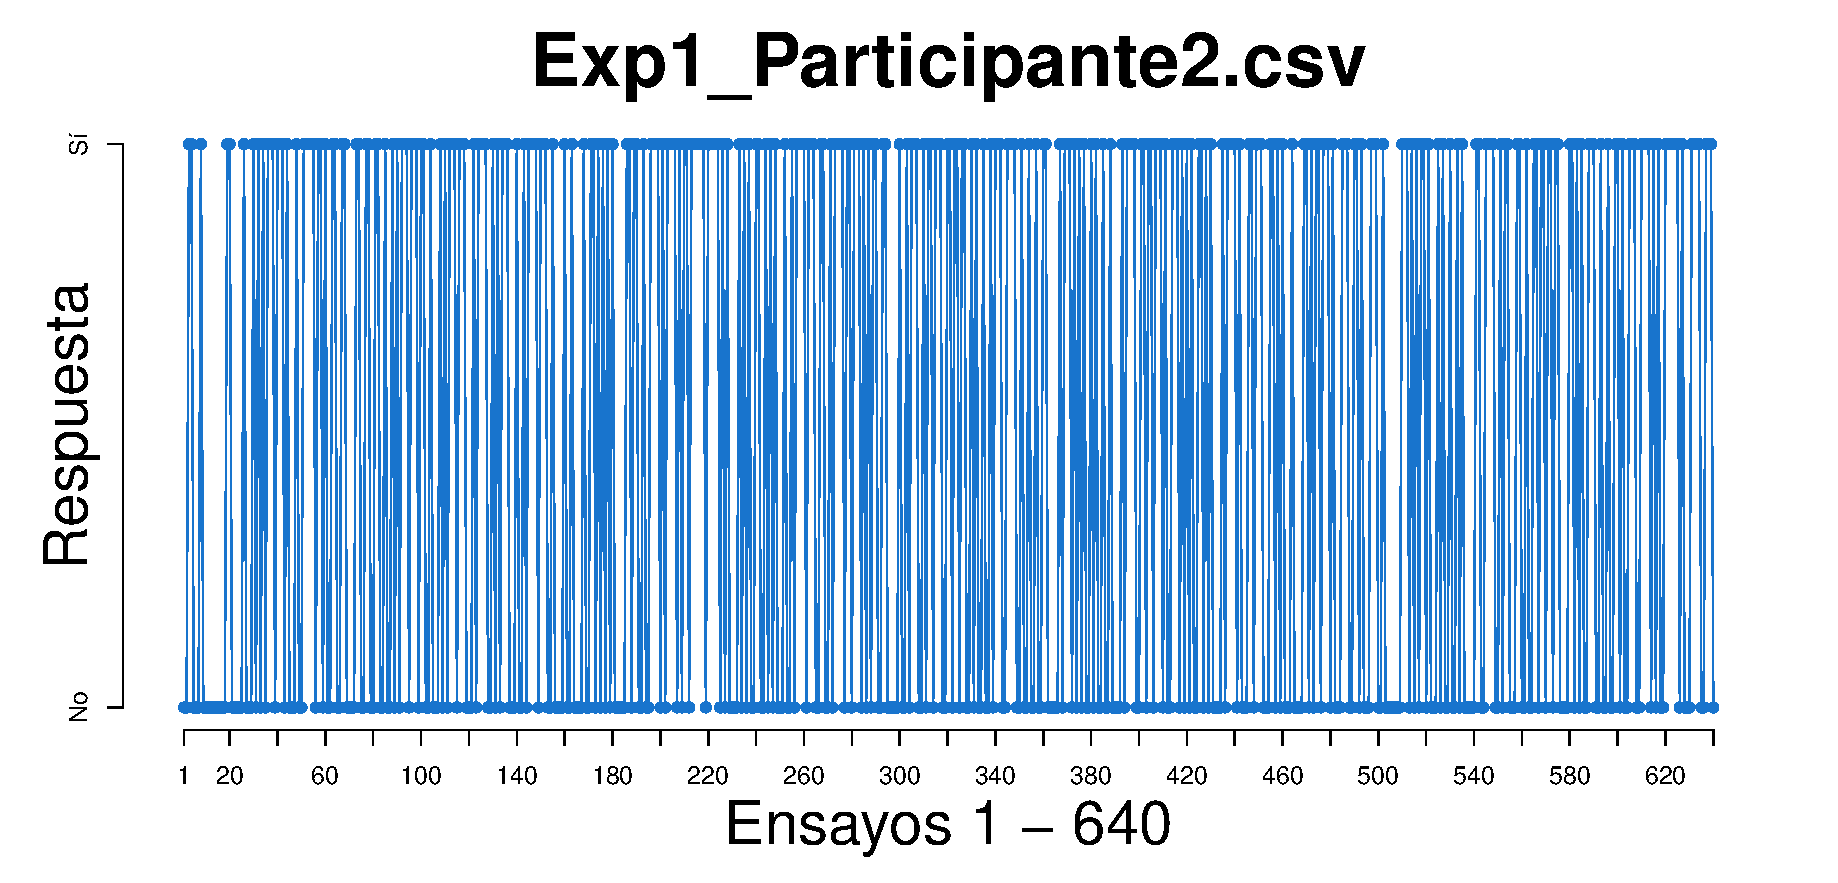
\includegraphics[width=9cm, height=5cm]{Figures/Response_Exp1_P2} 
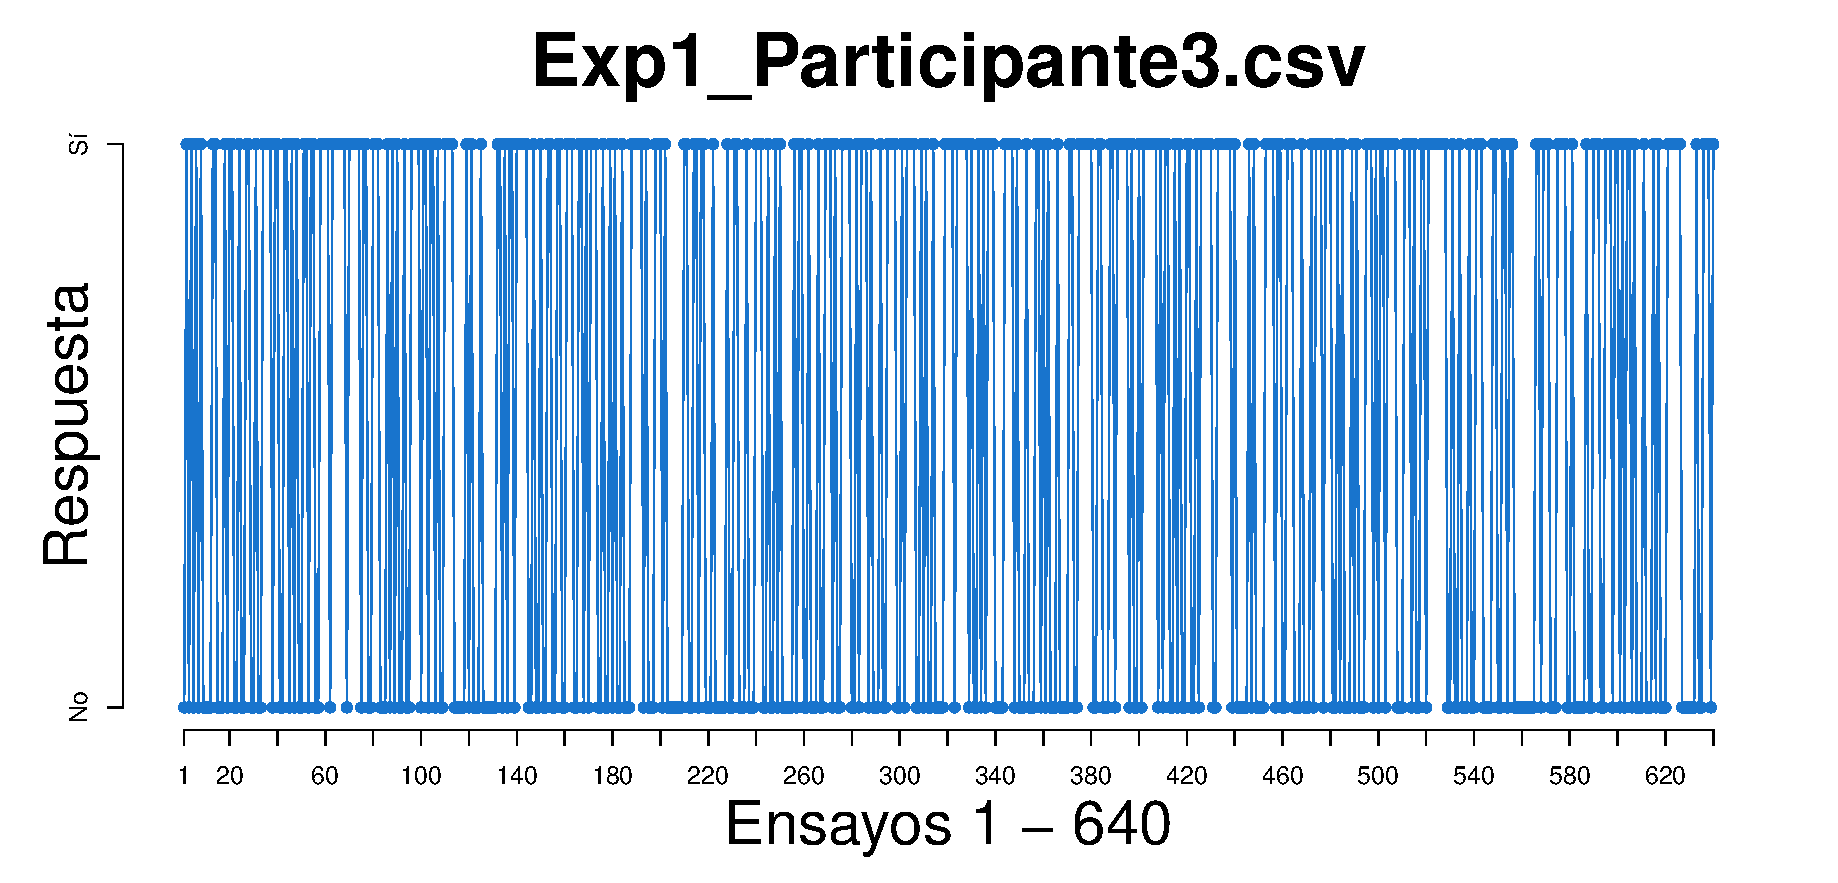
\includegraphics[width=9cm, height=5cm]{Figures/Response_Exp1_P3} 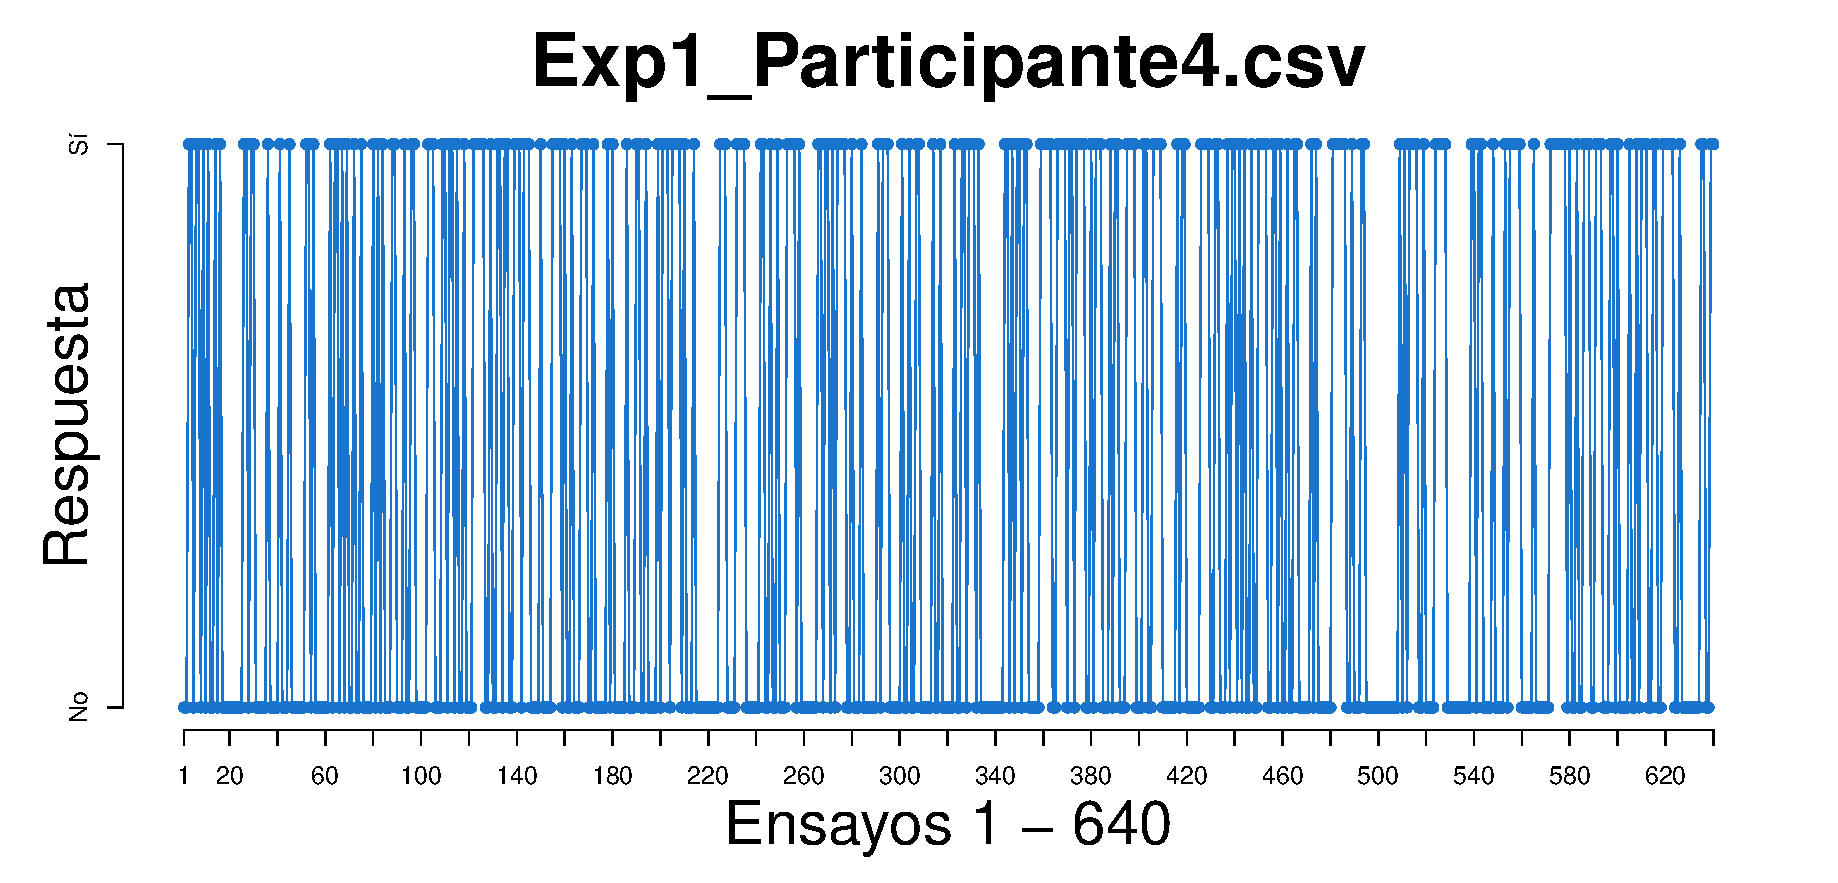
\includegraphics[width=9cm, height=5cm]{Figures/Response_Exp1_P4} 
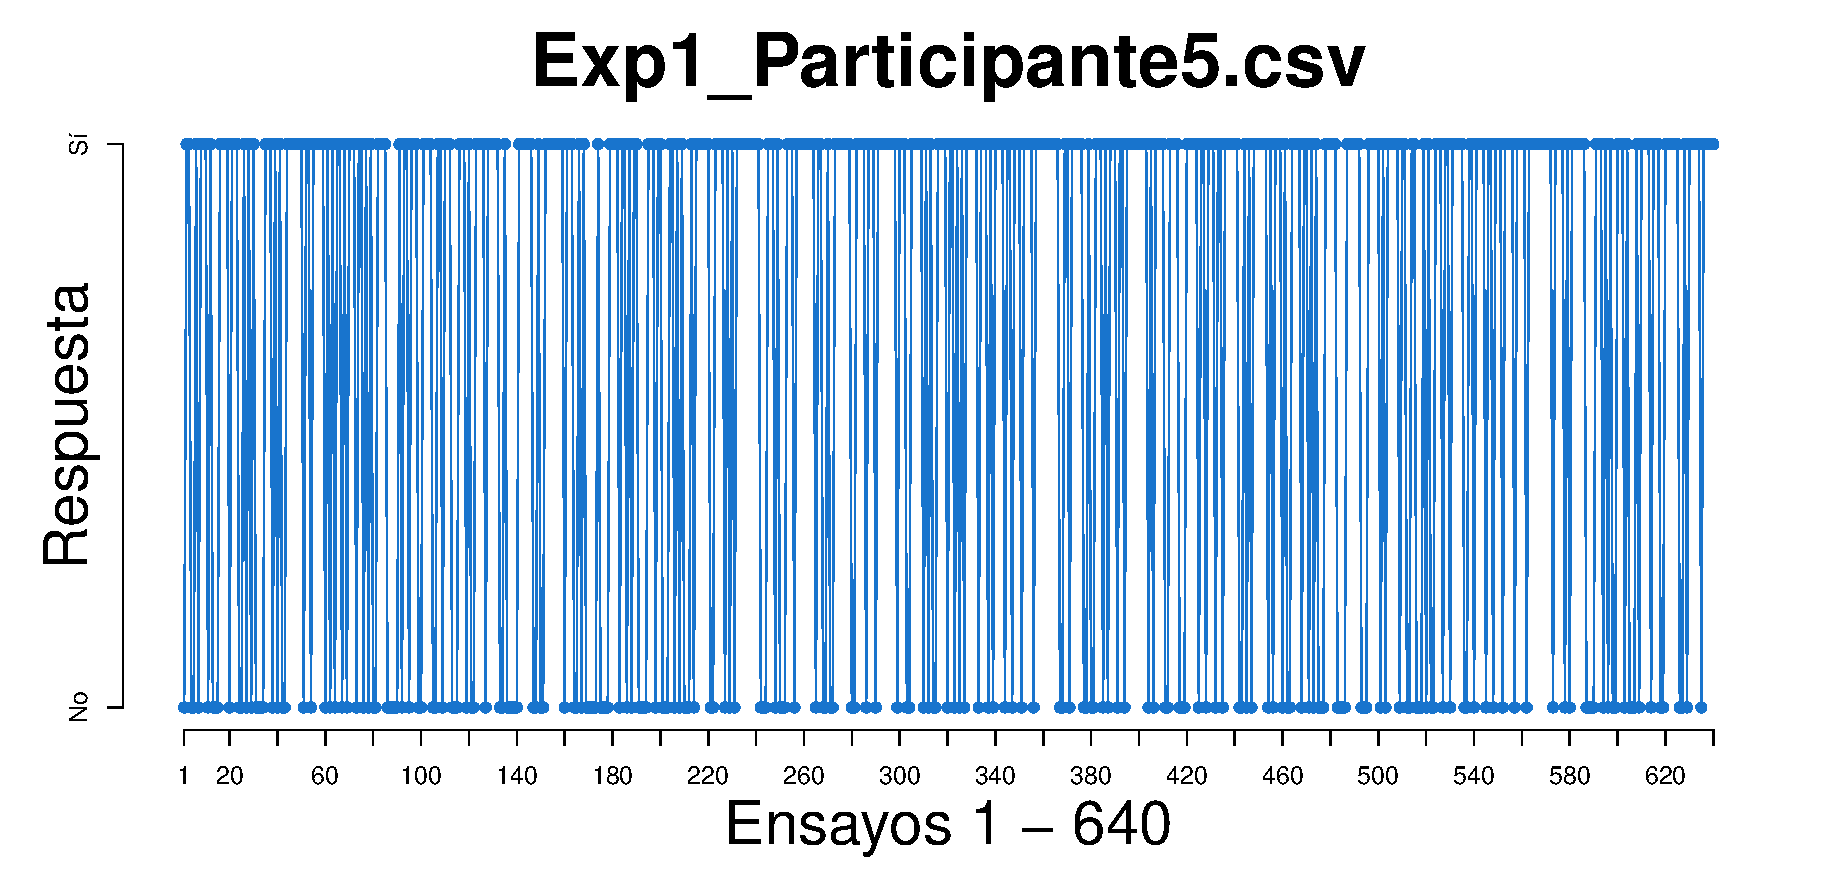
\includegraphics[width=9cm, height=5cm]{Figures/Response_Exp1_P5} 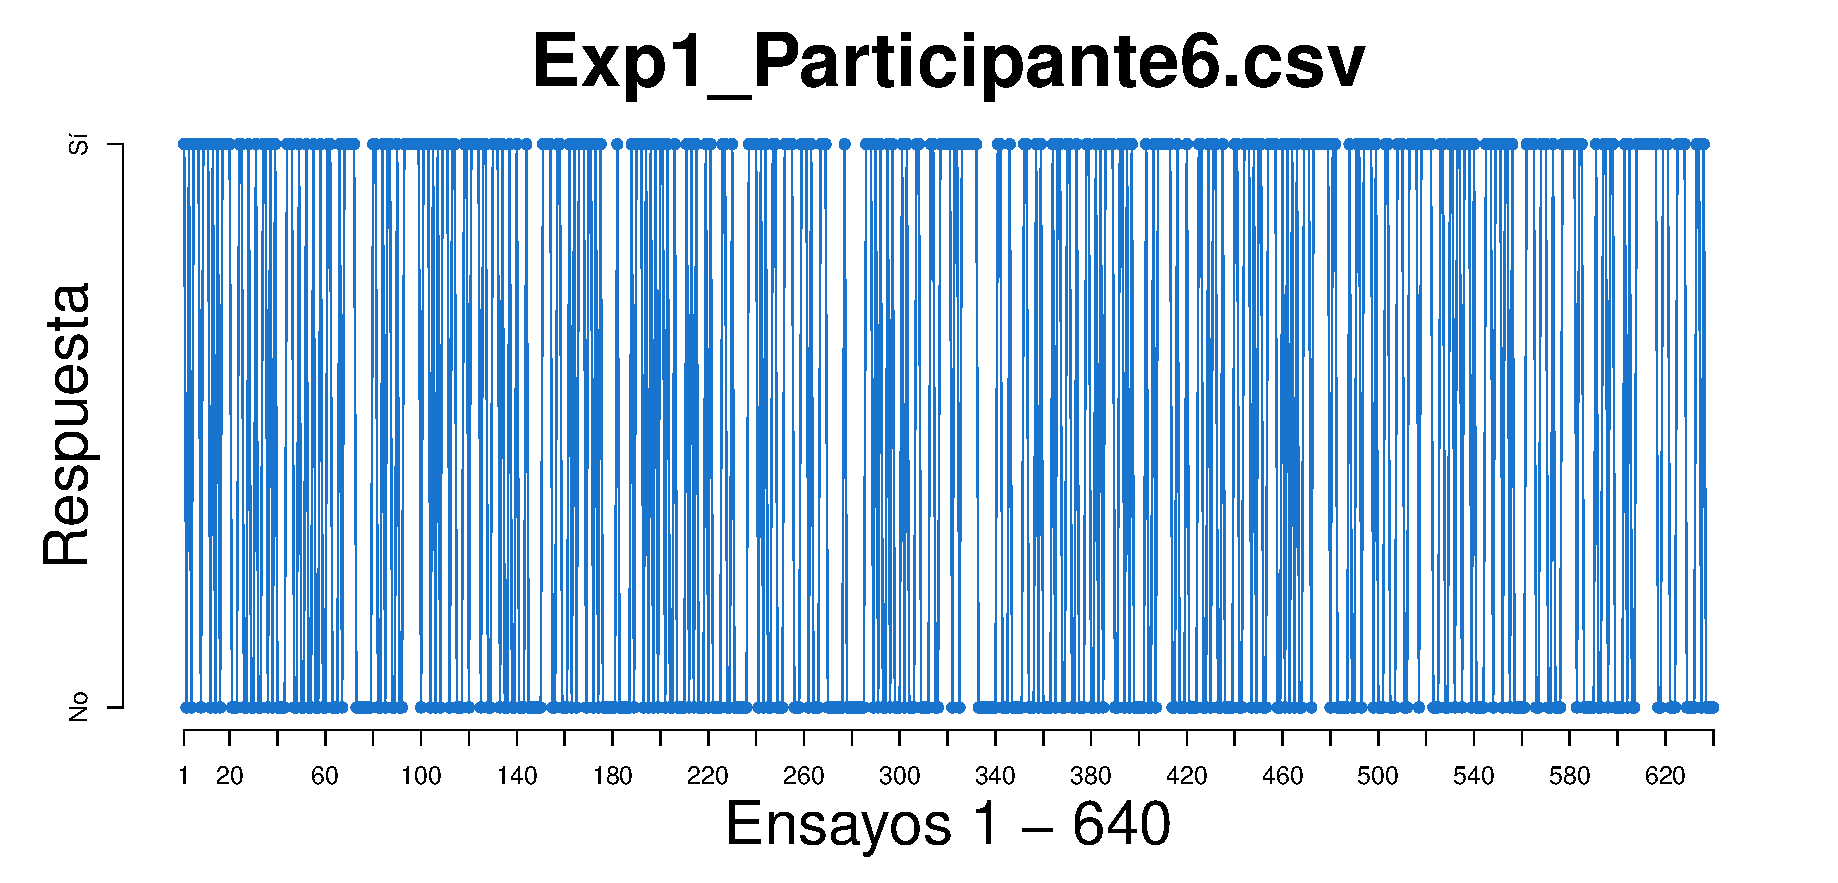
\includegraphics[width=9cm, height=5cm]{Figures/Response_Exp1_P6}
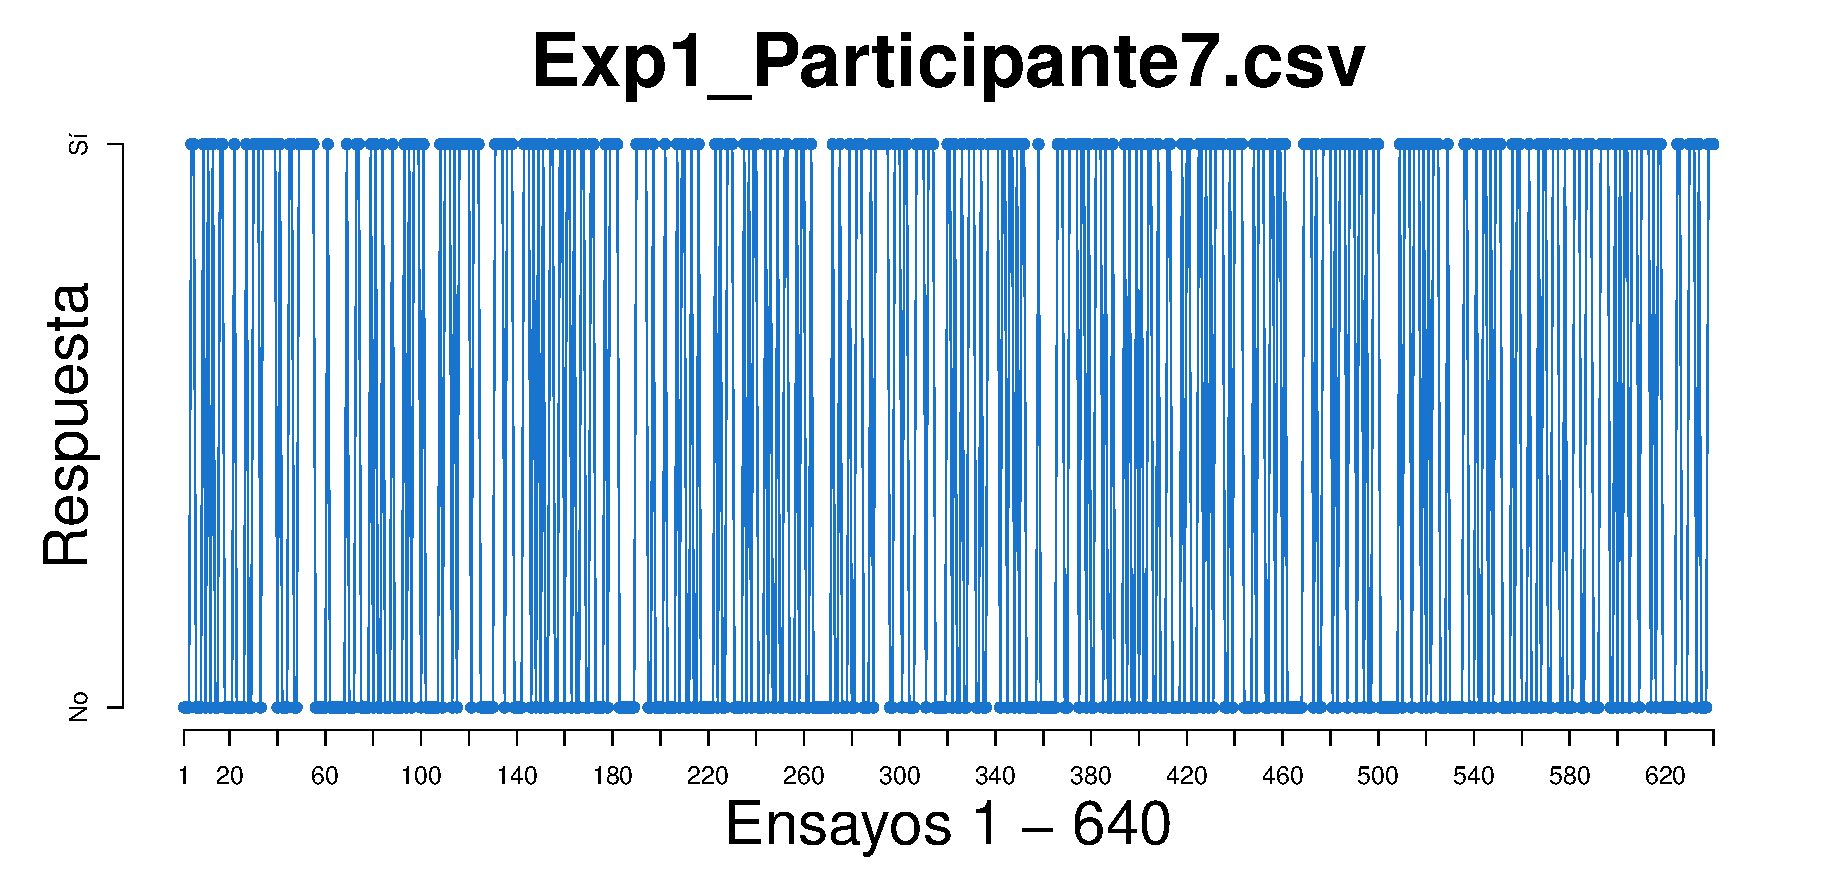
\includegraphics[width=9cm, height=5cm]{Figures/Response_Exp1_P7} 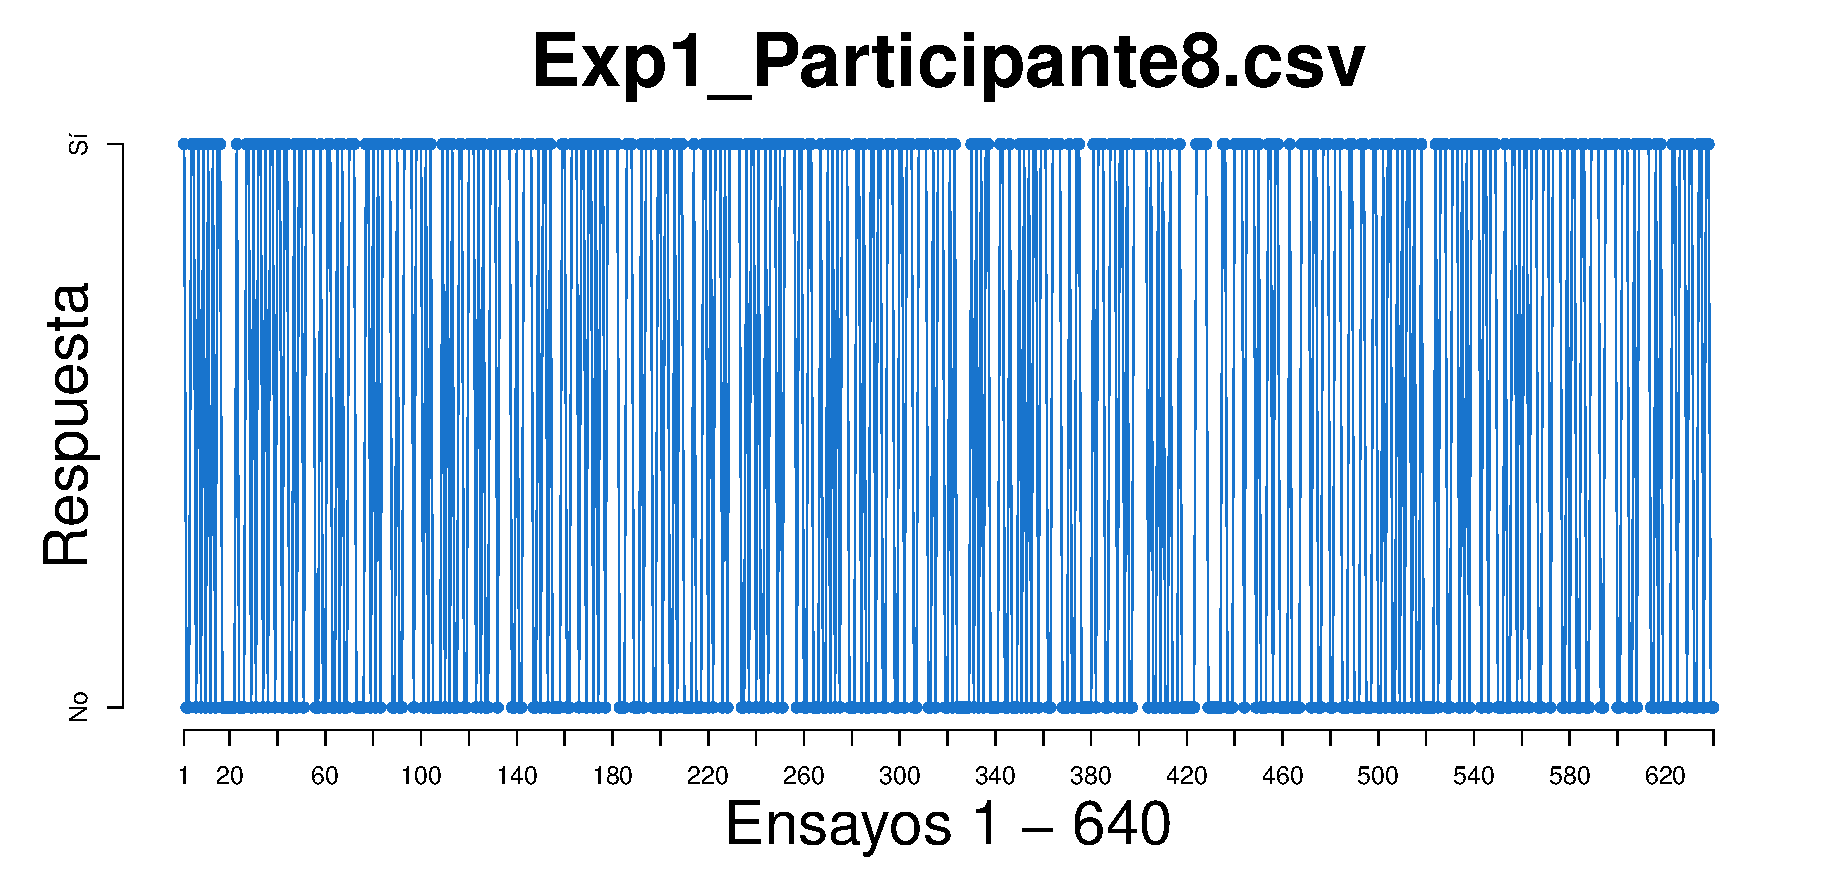
\includegraphics[width=9cm, height=5cm]{Figures/Response_Exp1_P8} 
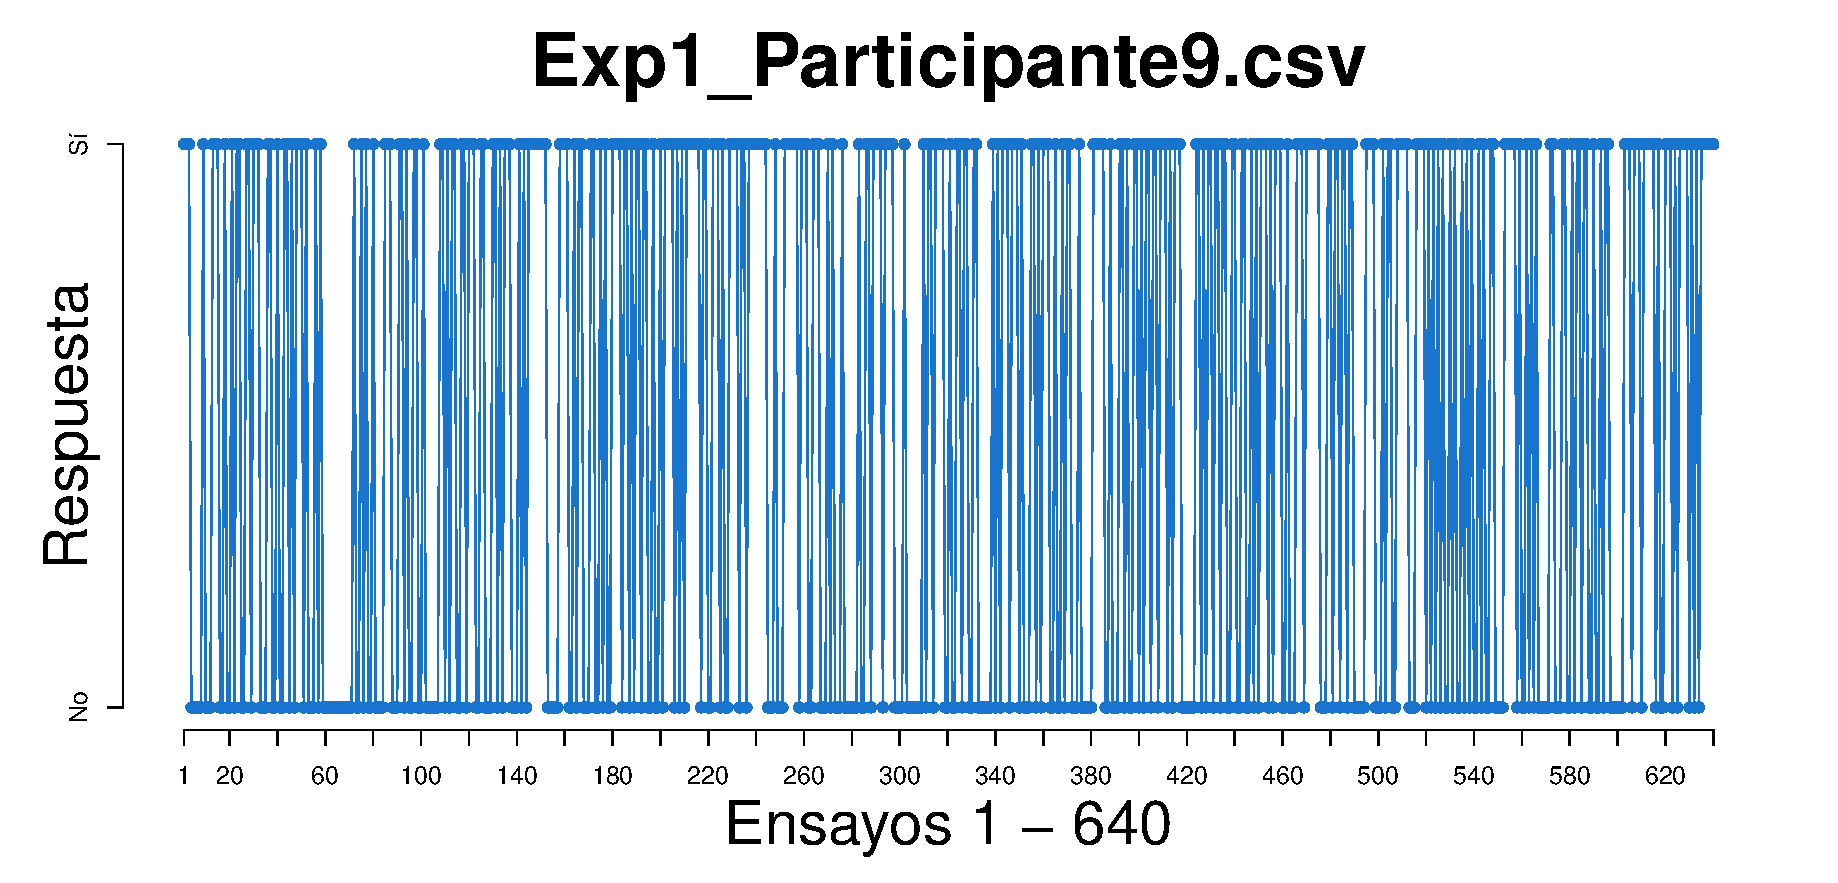
\includegraphics[width=9cm, height=5cm]{Figures/Response_Exp1_P9}
\end{figure}
\vfill .
\begin{figure}[th]
\begin{center}
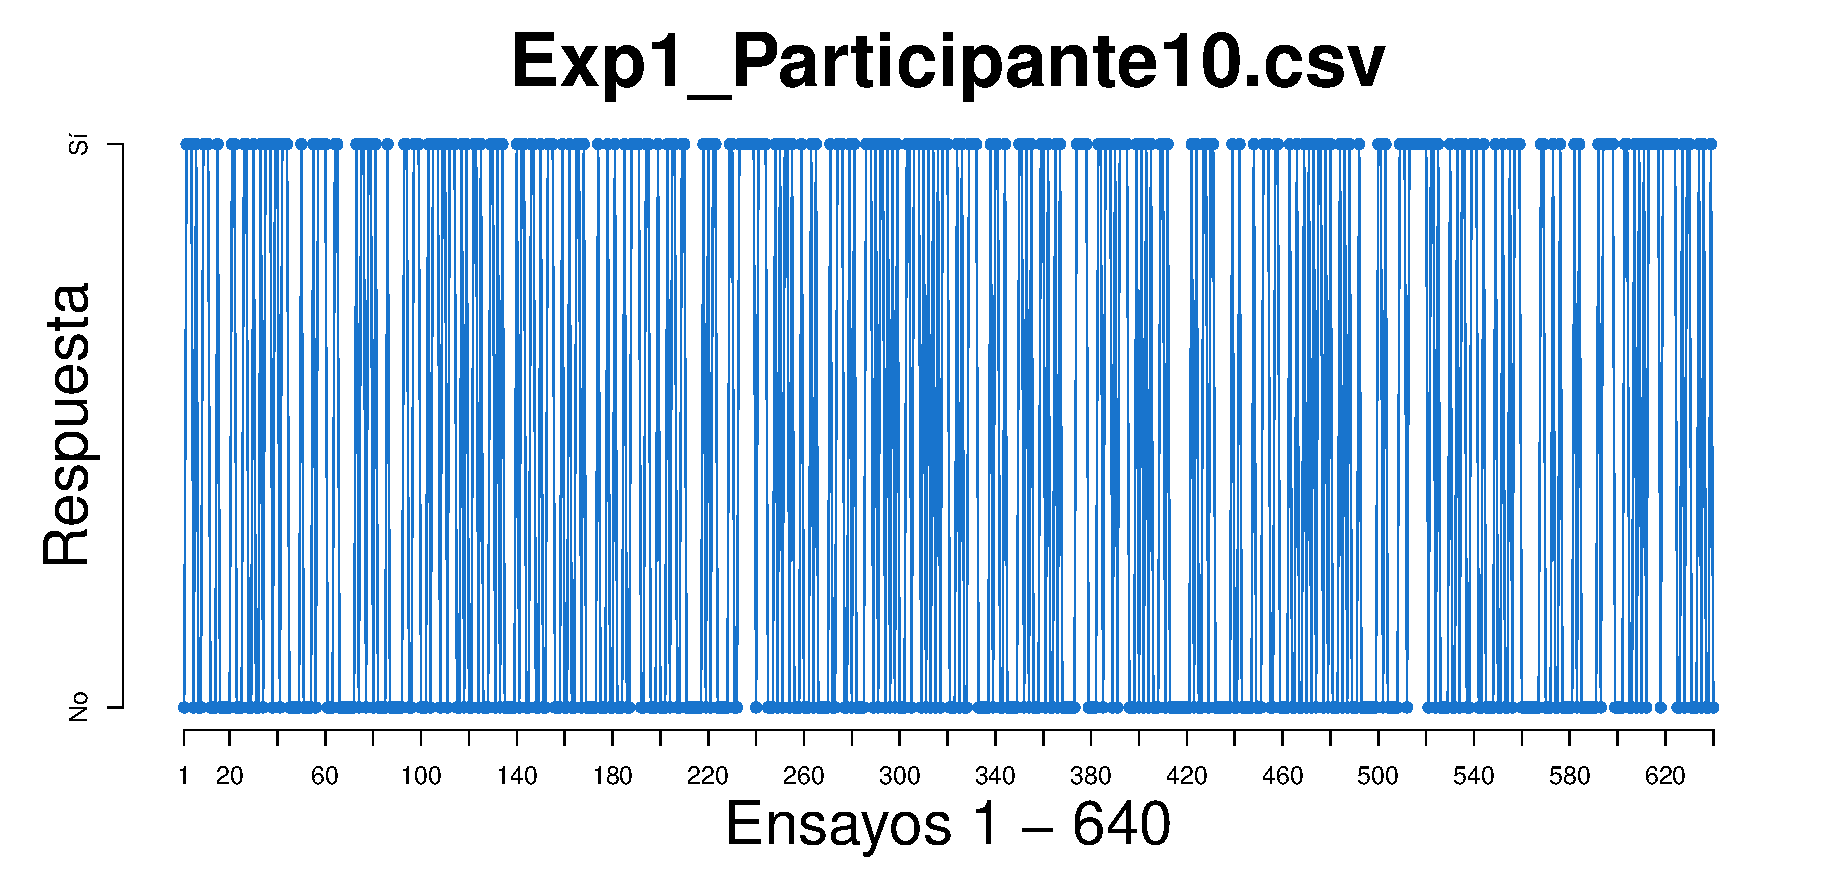
\includegraphics[width=8cm, height=4cm]{Figures/Response_Exp1_P10} 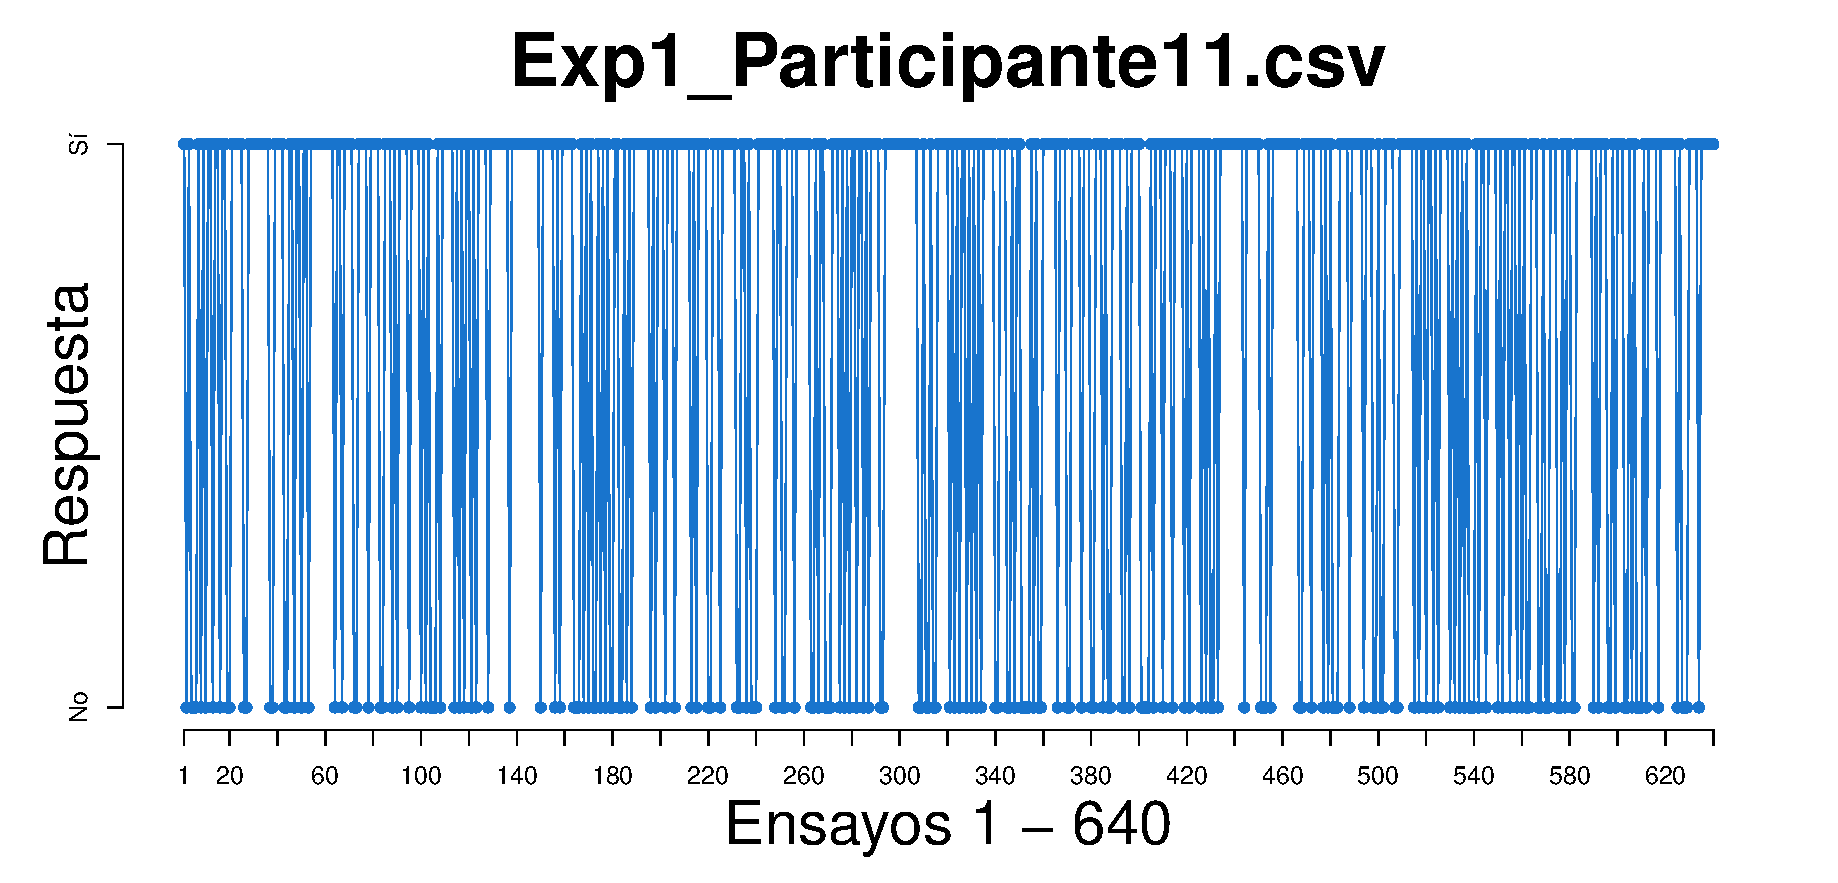
\includegraphics[width=8cm, height=4cm]{Figures/Response_Exp1_P11} 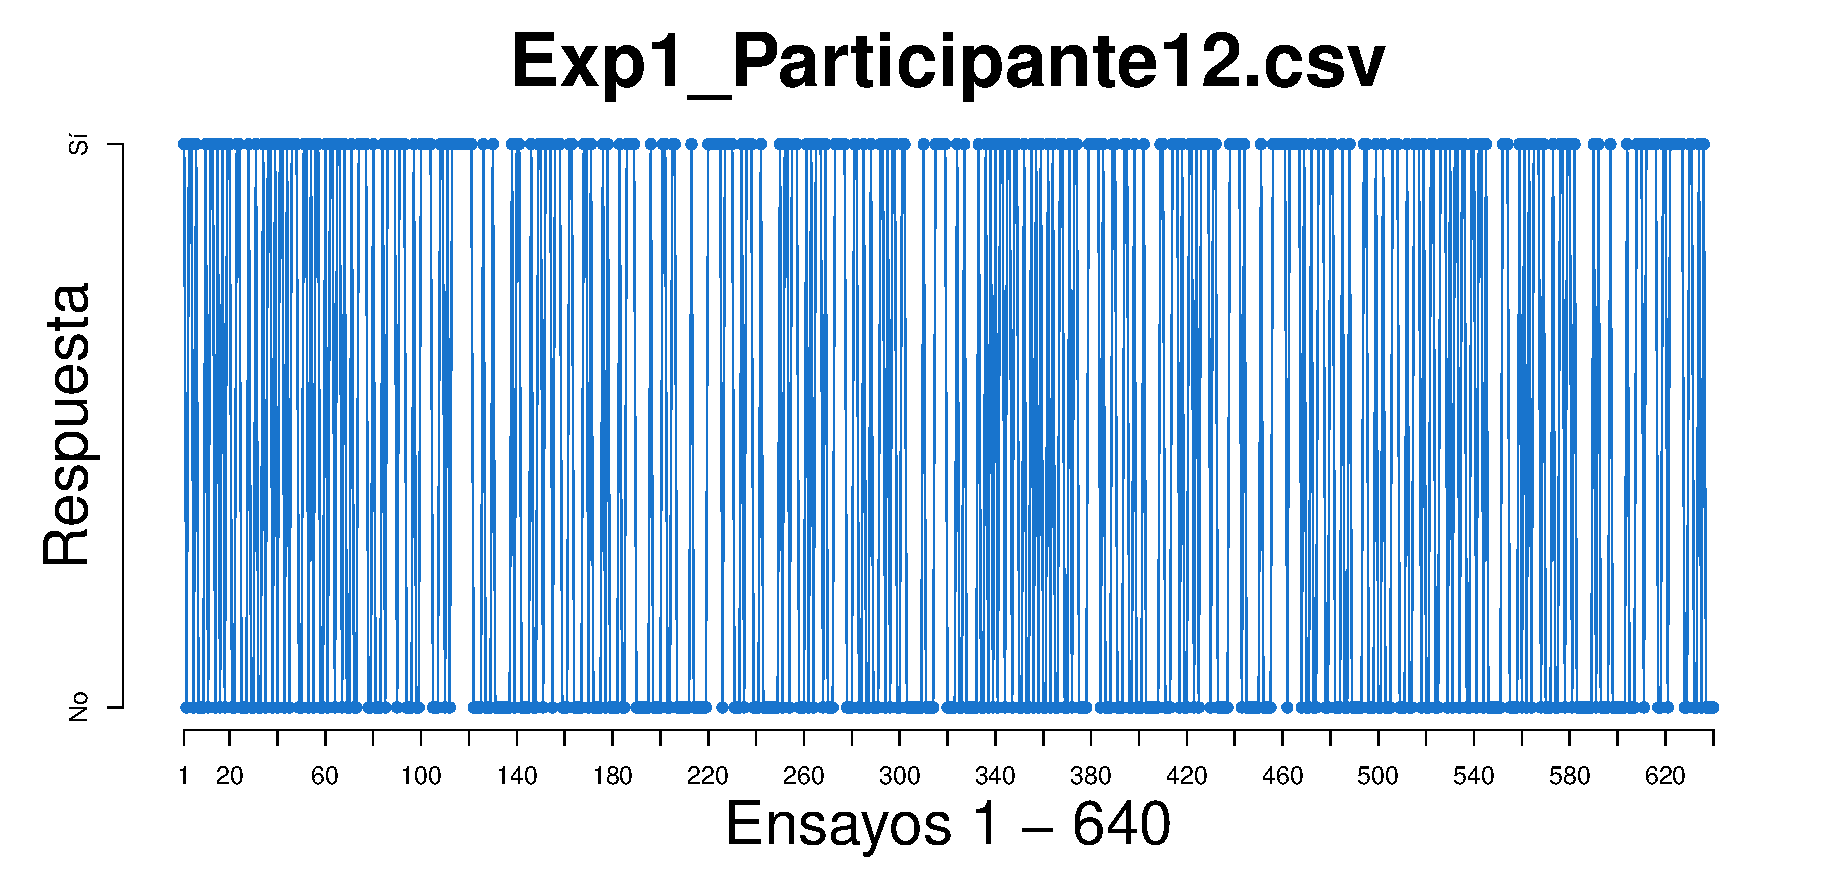
\includegraphics[width=8cm, height=4cm]{Figures/Response_Exp1_P12}
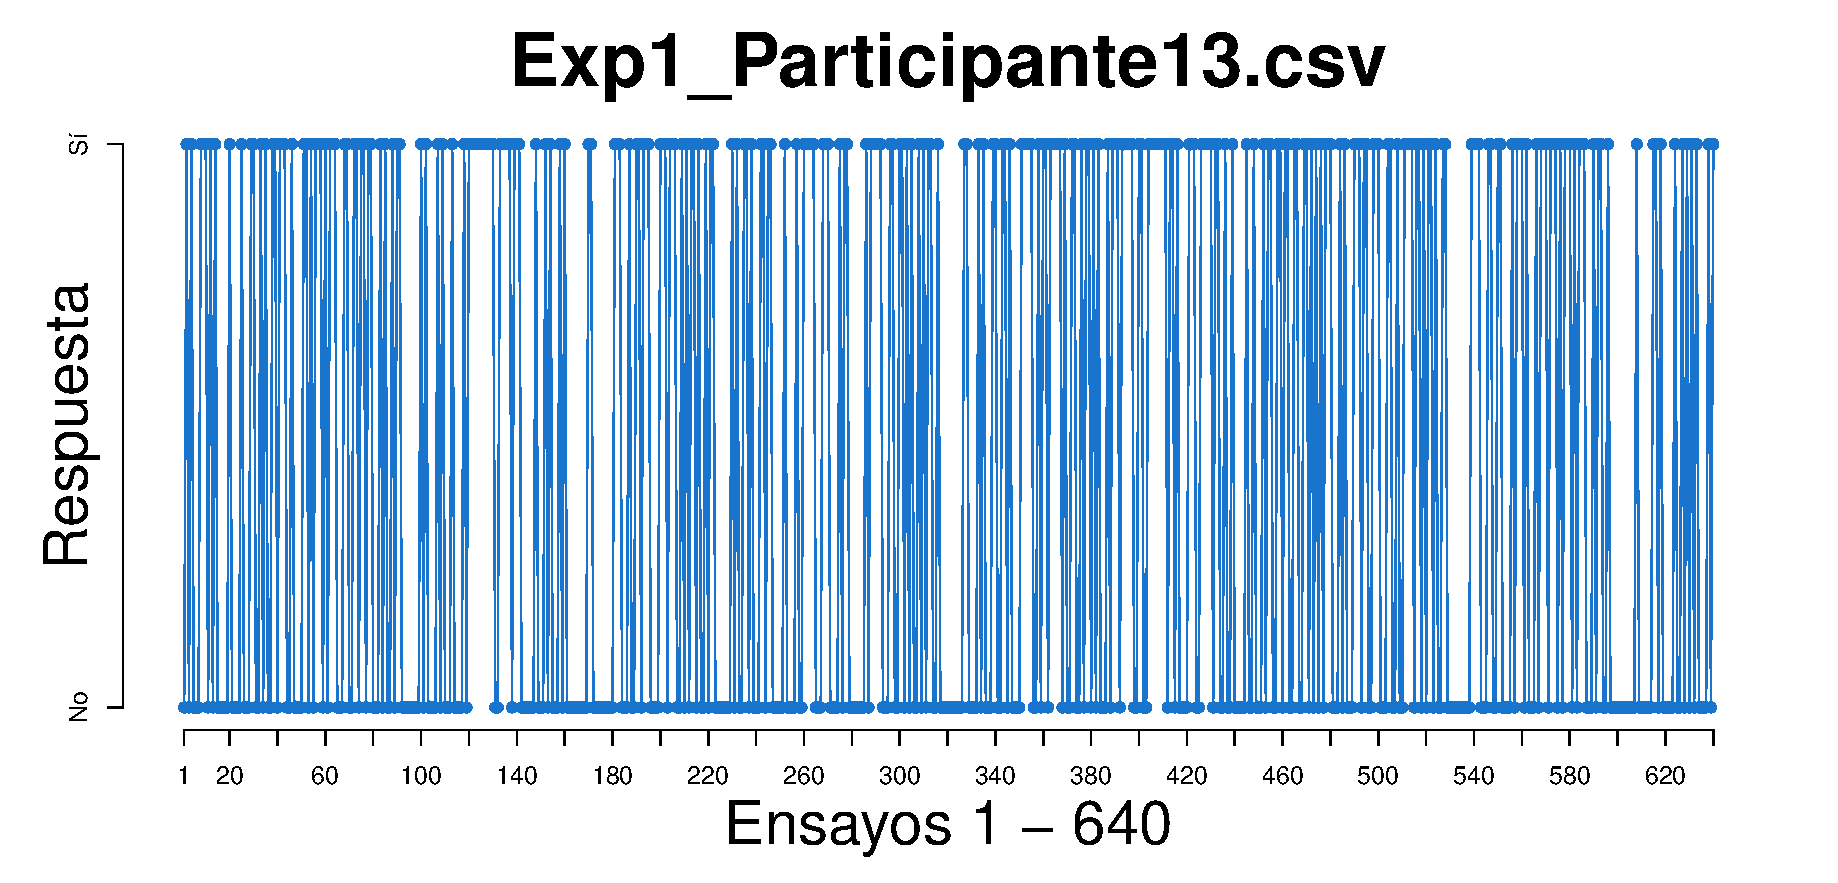
\includegraphics[width=8cm, height=4cm]{Figures/Response_Exp1_P13} 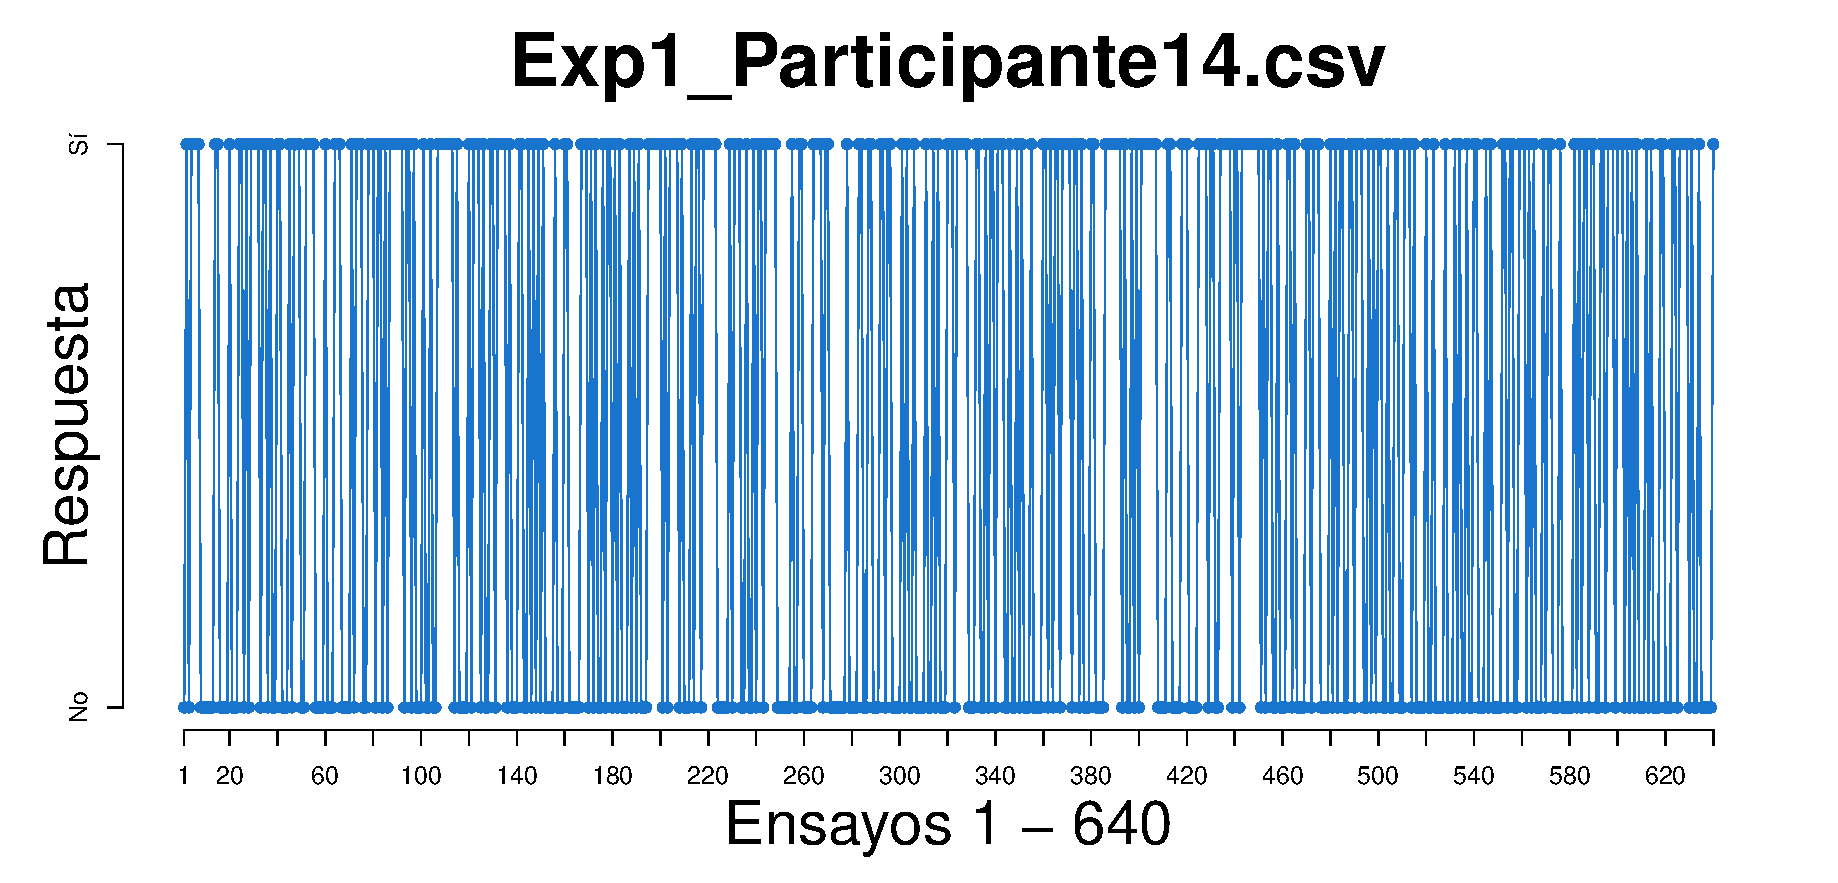
\includegraphics[width=8cm, height=4cm]{Figures/Response_Exp1_P14} 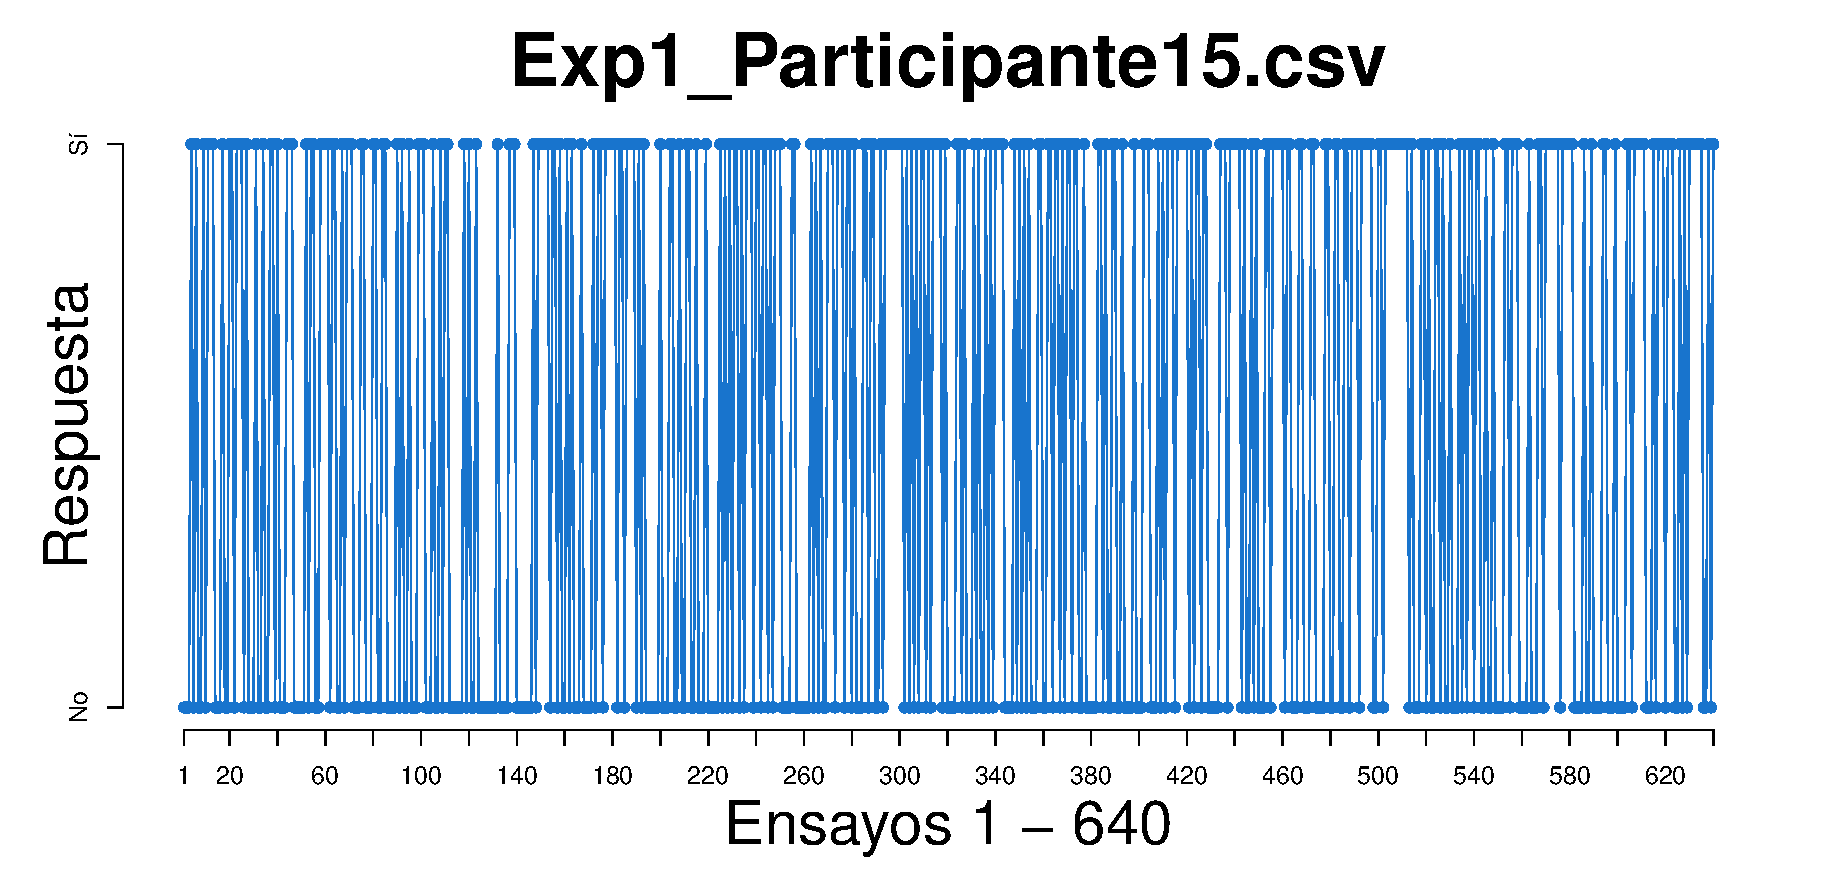
\includegraphics[width=8cm, height=4cm]{Figures/Response_Exp1_P15}
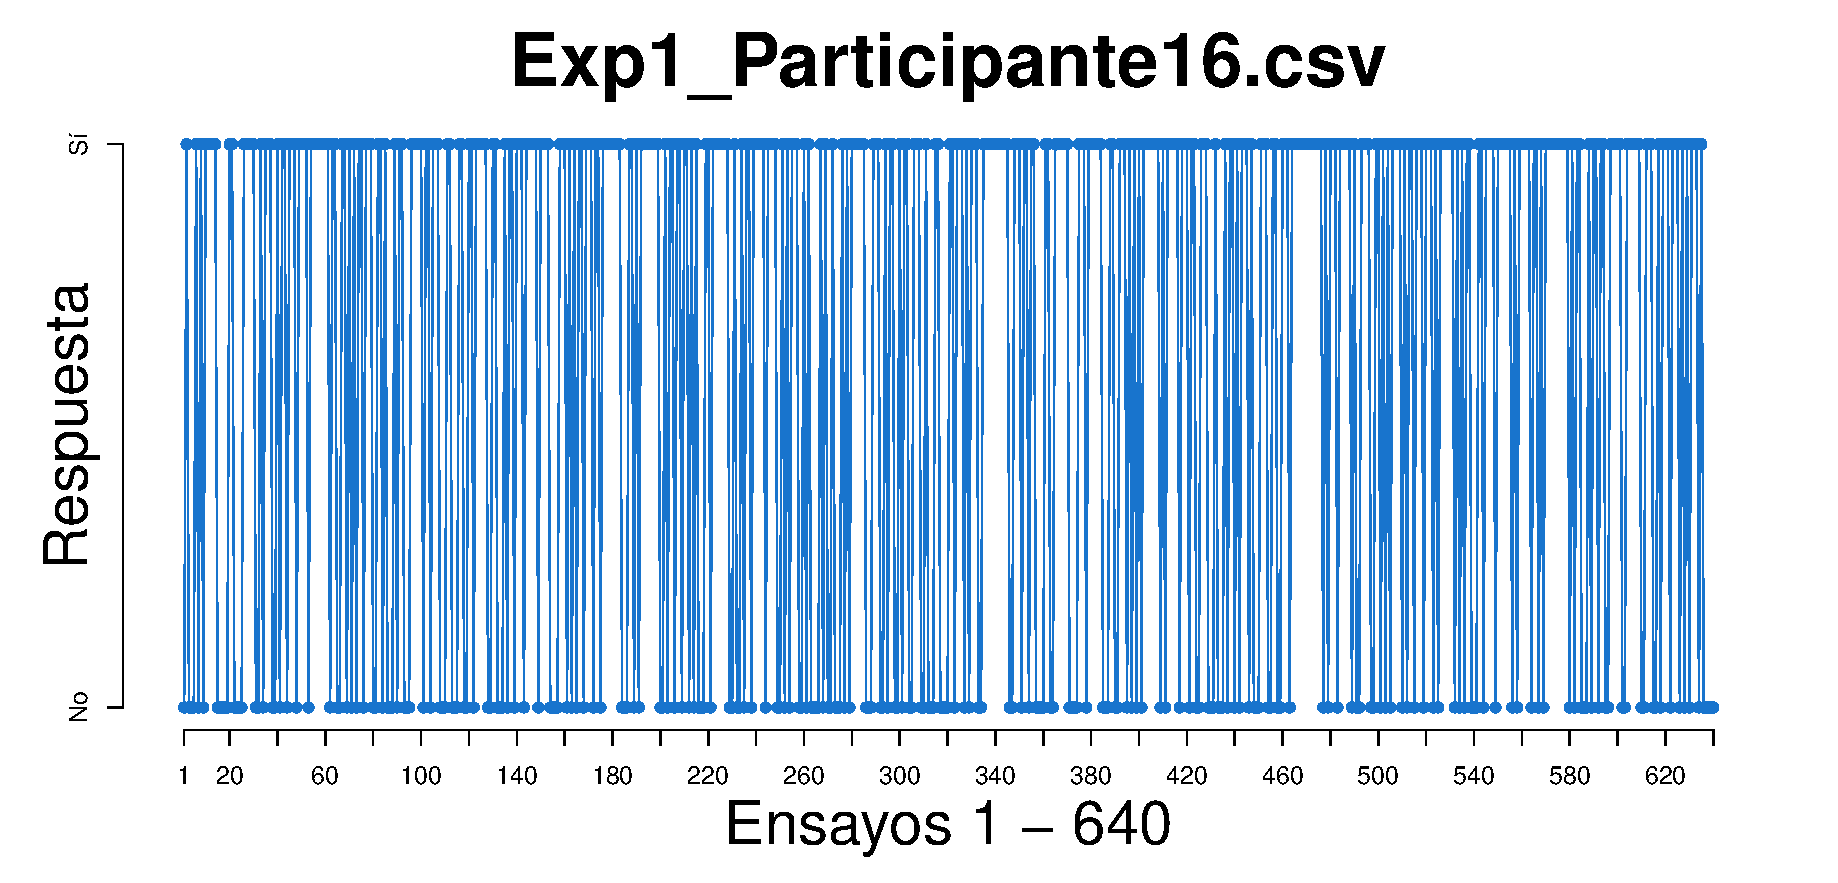
\includegraphics[width=8cm, height=4cm]{Figures/Response_Exp1_P16} 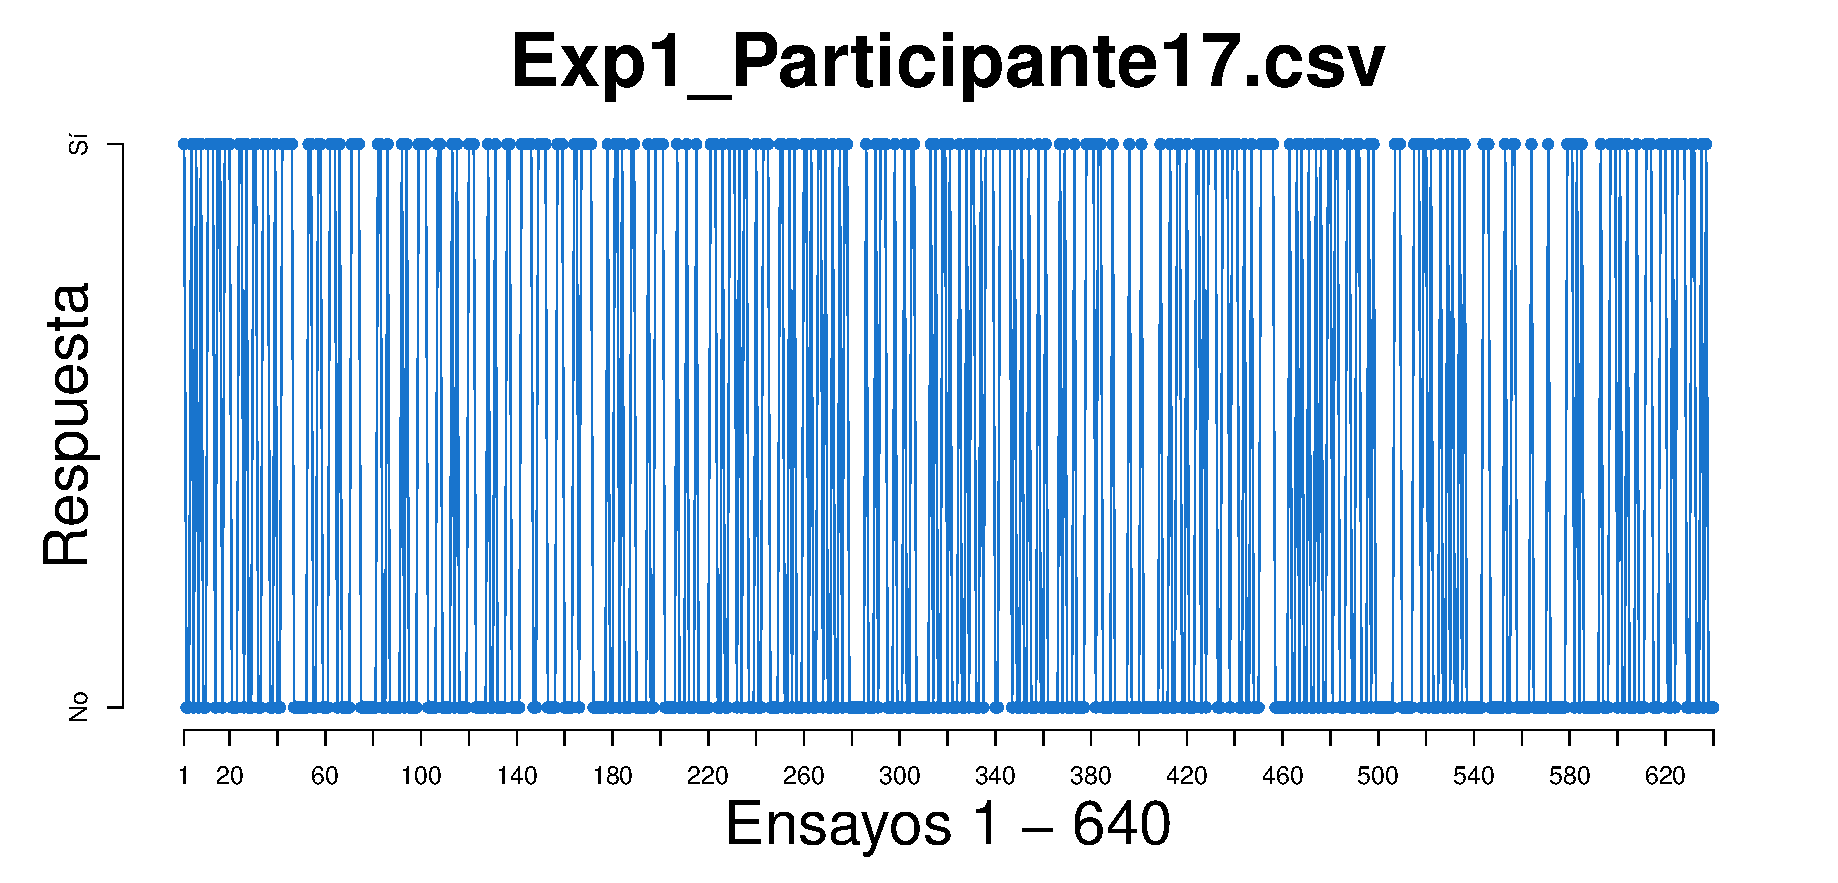
\includegraphics[width=8cm, height=4cm]{Figures/Response_Exp1_P17} 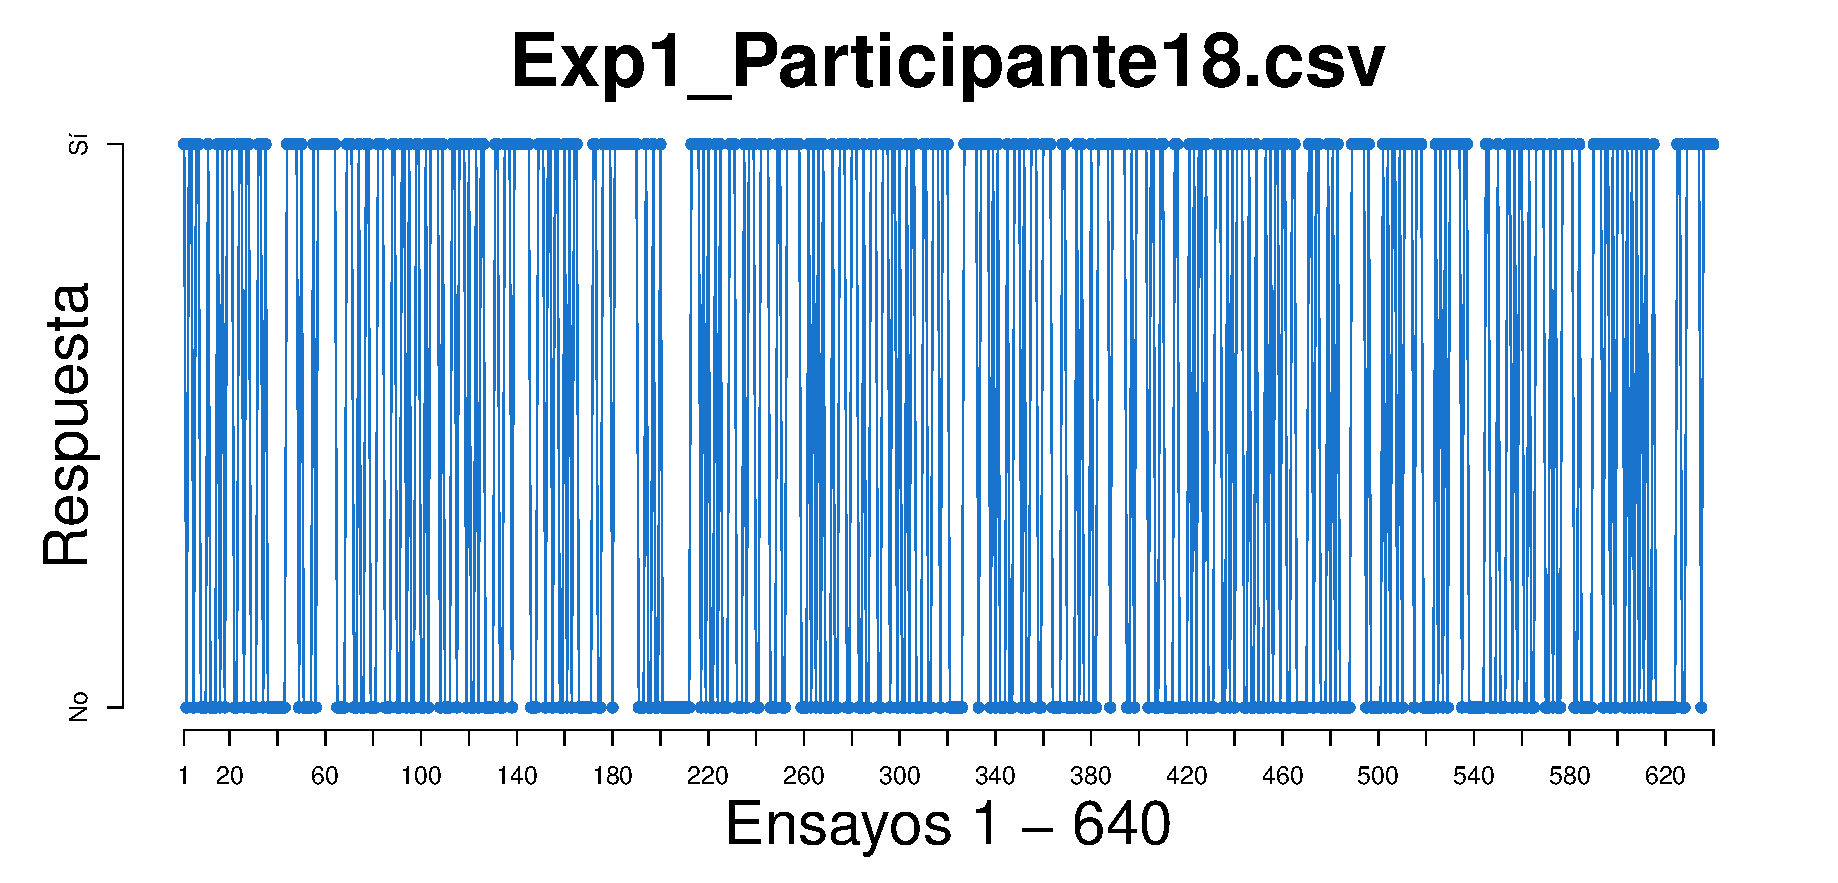
\includegraphics[width=8cm, height=4cm]{Figures/Response_Exp1_P18}
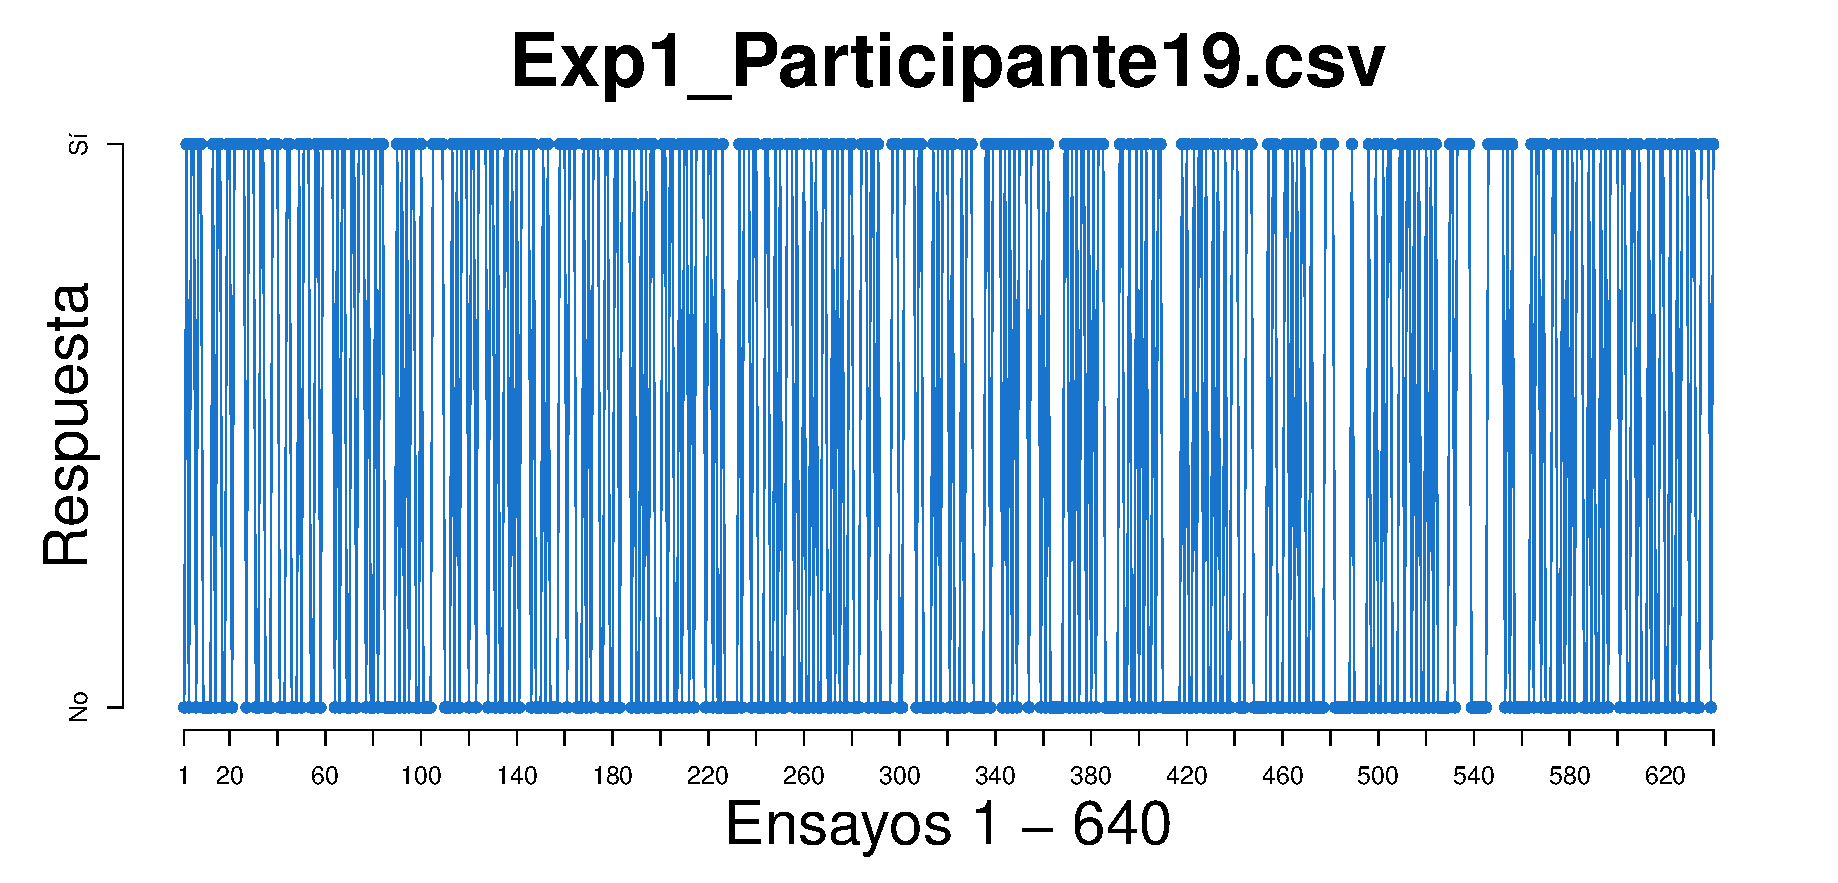
\includegraphics[width=8cm, height=4cm]{Figures/Response_Exp1_P19} \hspace{2cm} 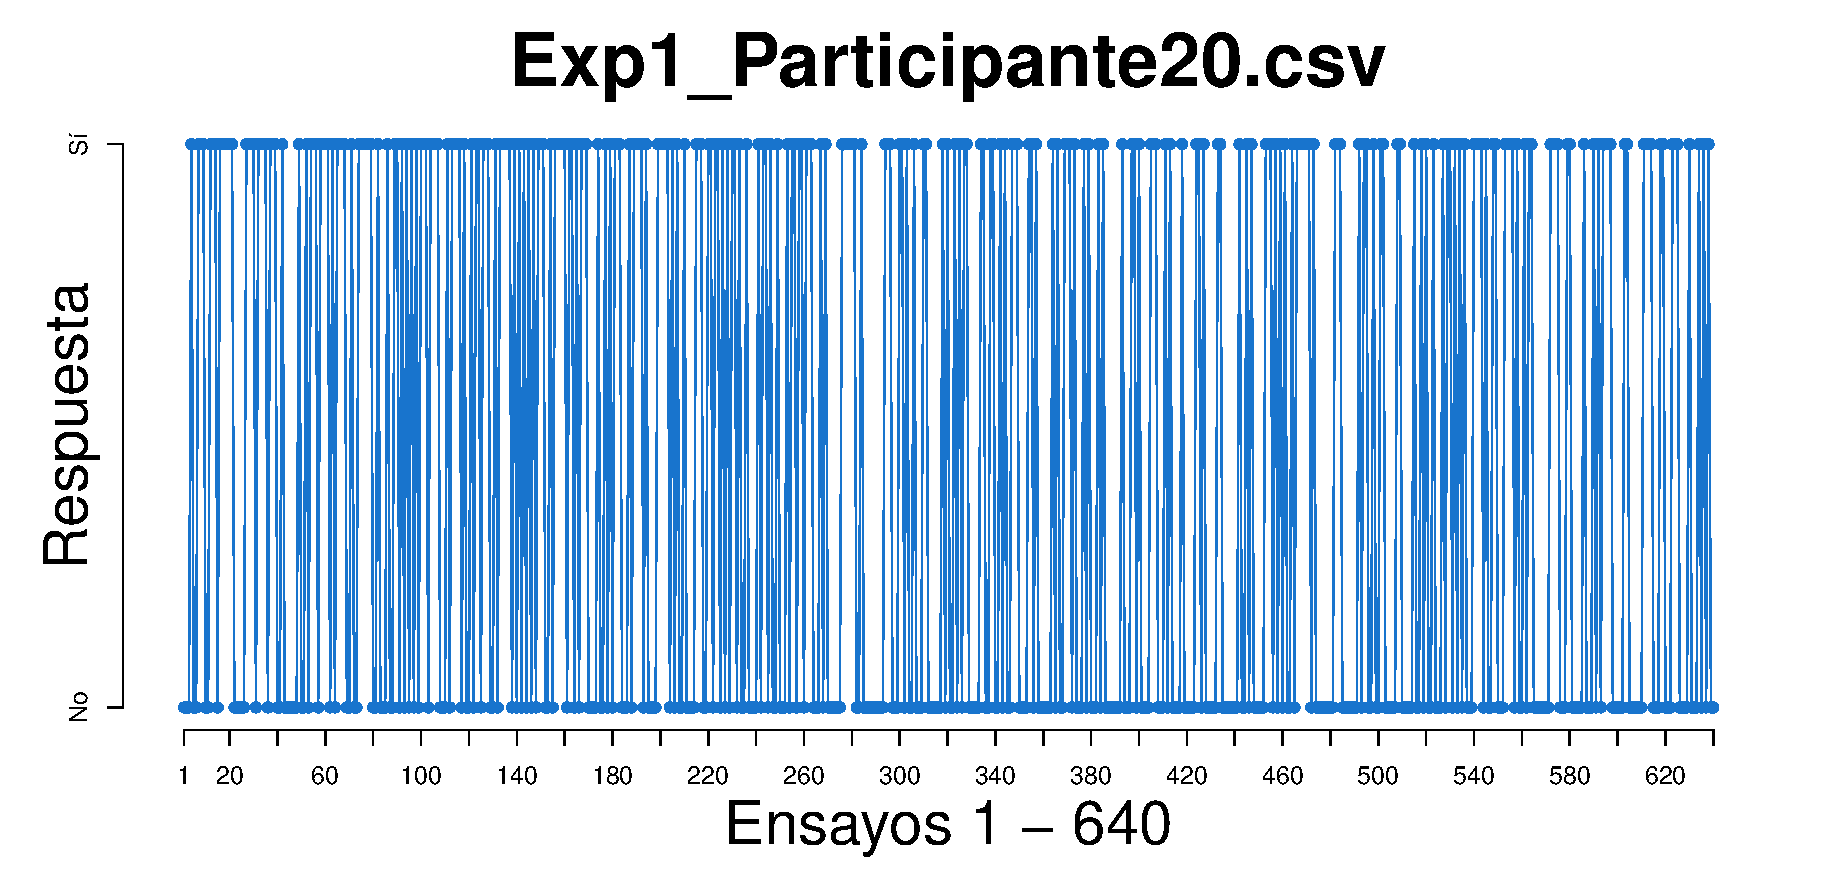
\includegraphics[width=8cm, height=4cm]{Figures/Response_Exp1_P20} 
\end{center}
\end{figure}
\clearpage



---
\vspace{3mm}
\begin{center}
{\LARGE \textbf{Respuestas a la tarea 'Sí/No' registradas en cada ensayo}}\\
{\small \textsc{(para comprobar que todas las opciones de respuesta se hayan utilizado)}}\\
\smallskip
\end{center}
\begin{center}
{\LARGE \textit{Experimento 2}}\\
\end{center}
\vspace{3mm}
\begin{figure}[th]
\centering
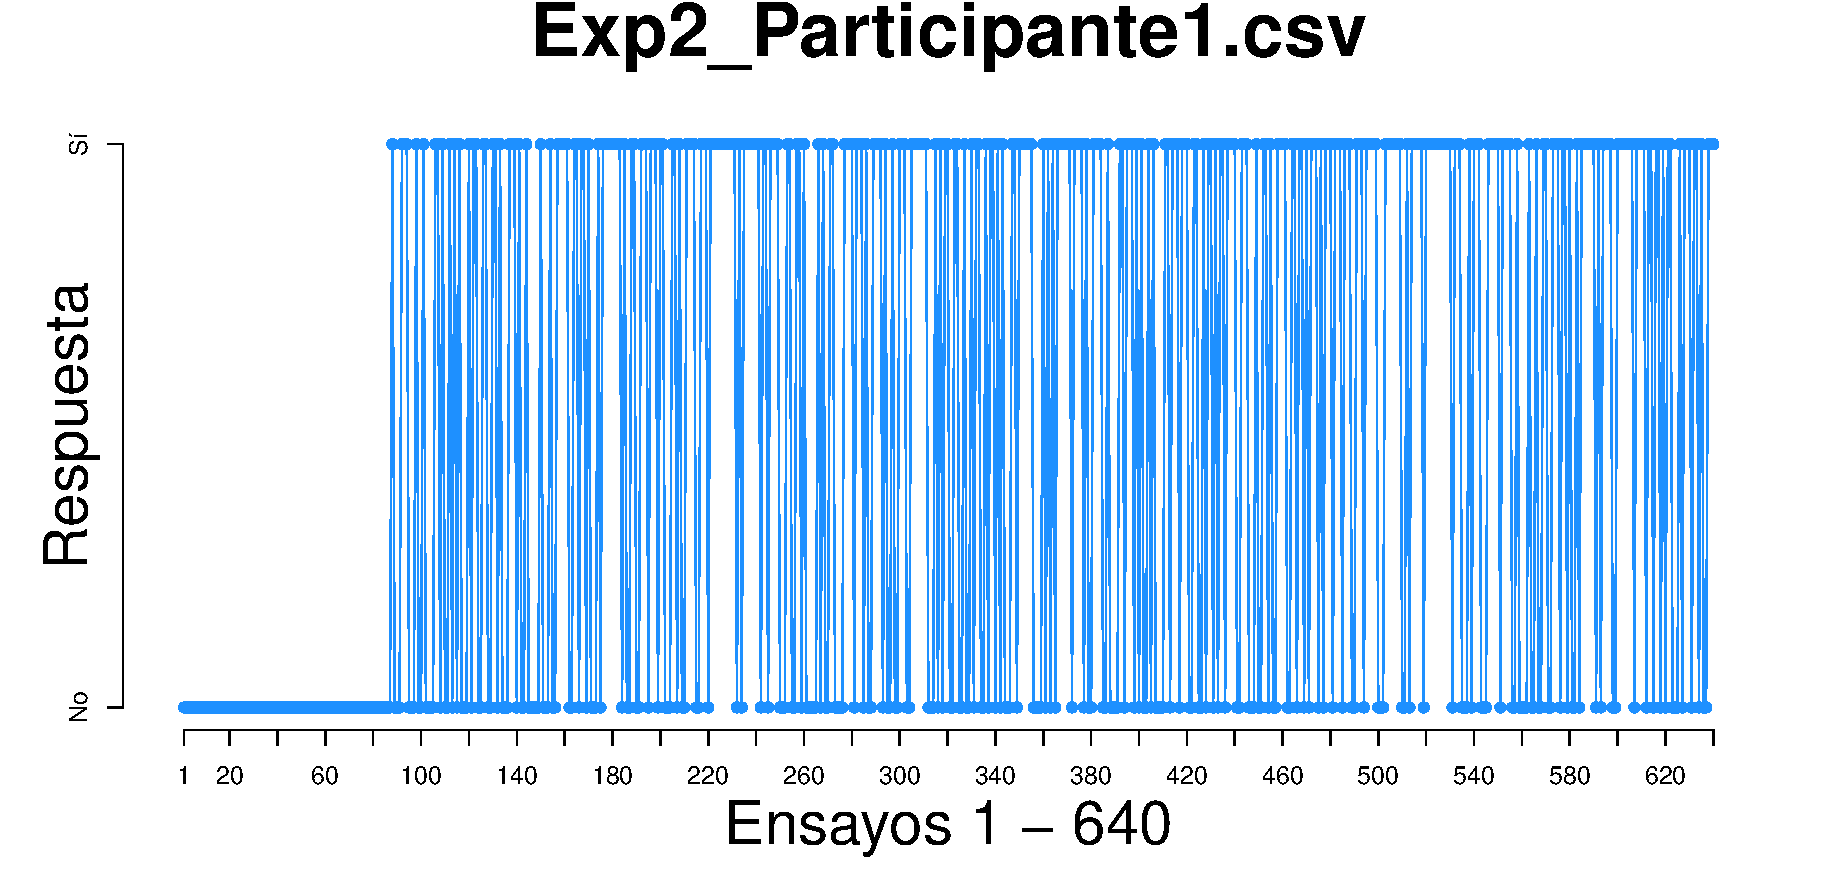
\includegraphics[width=9cm, height=5cm]{Figures/Response_Exp2_P1} 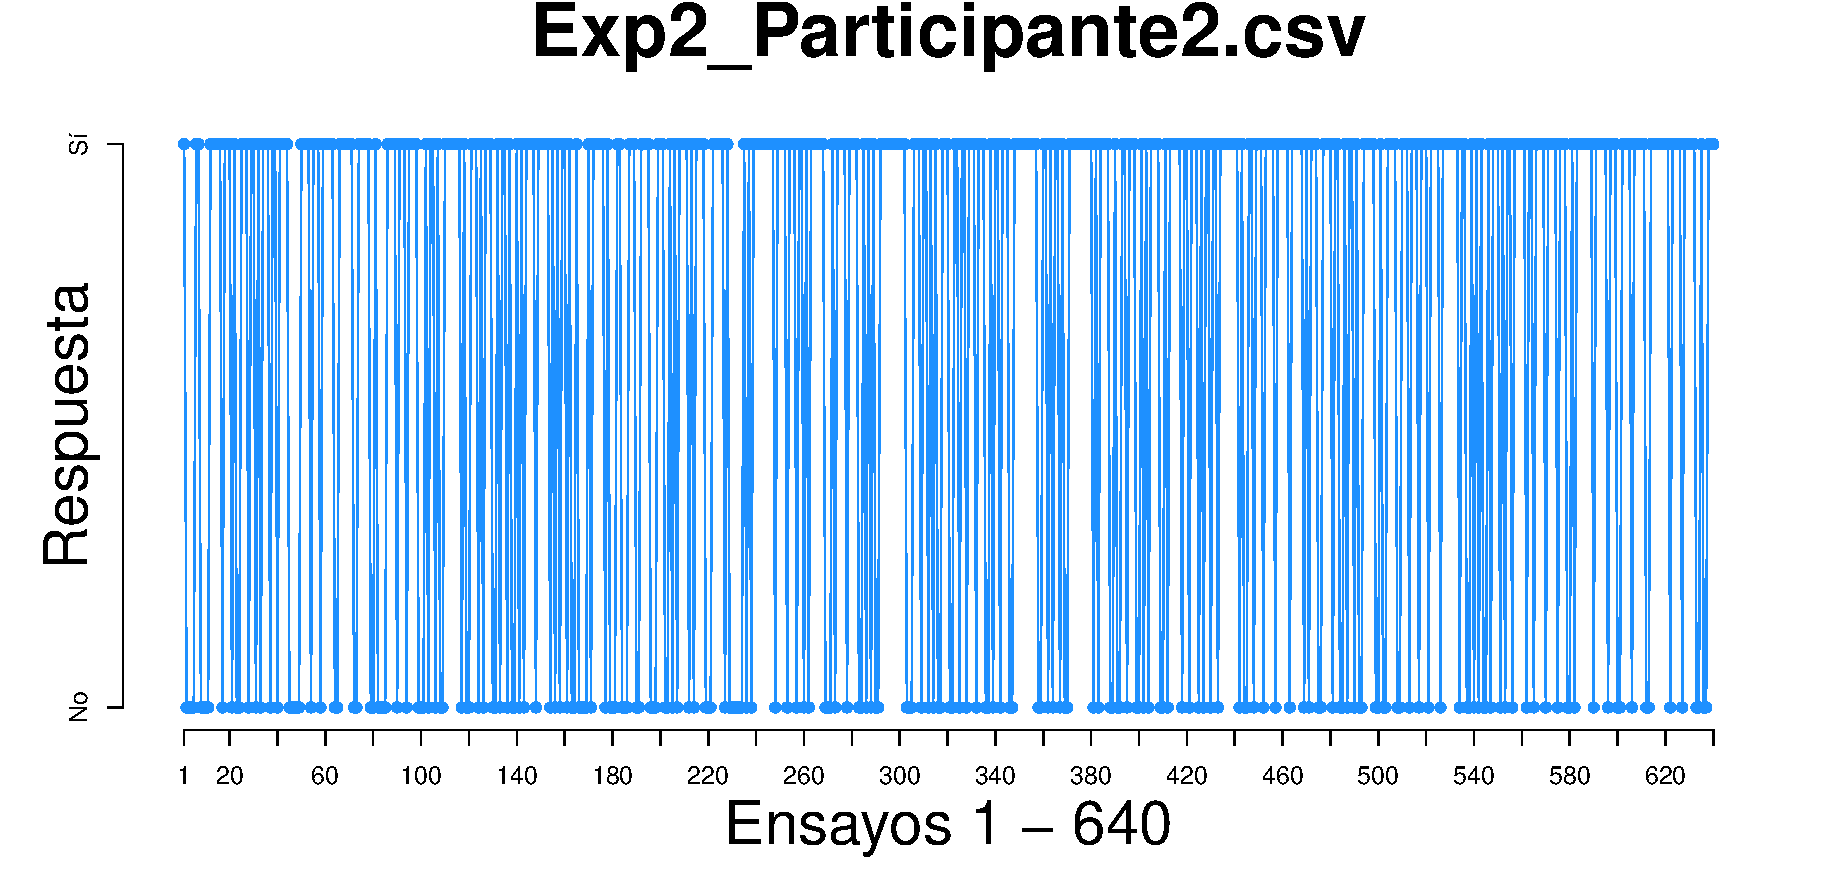
\includegraphics[width=9cm, height=5cm]{Figures/Response_Exp2_P2} 
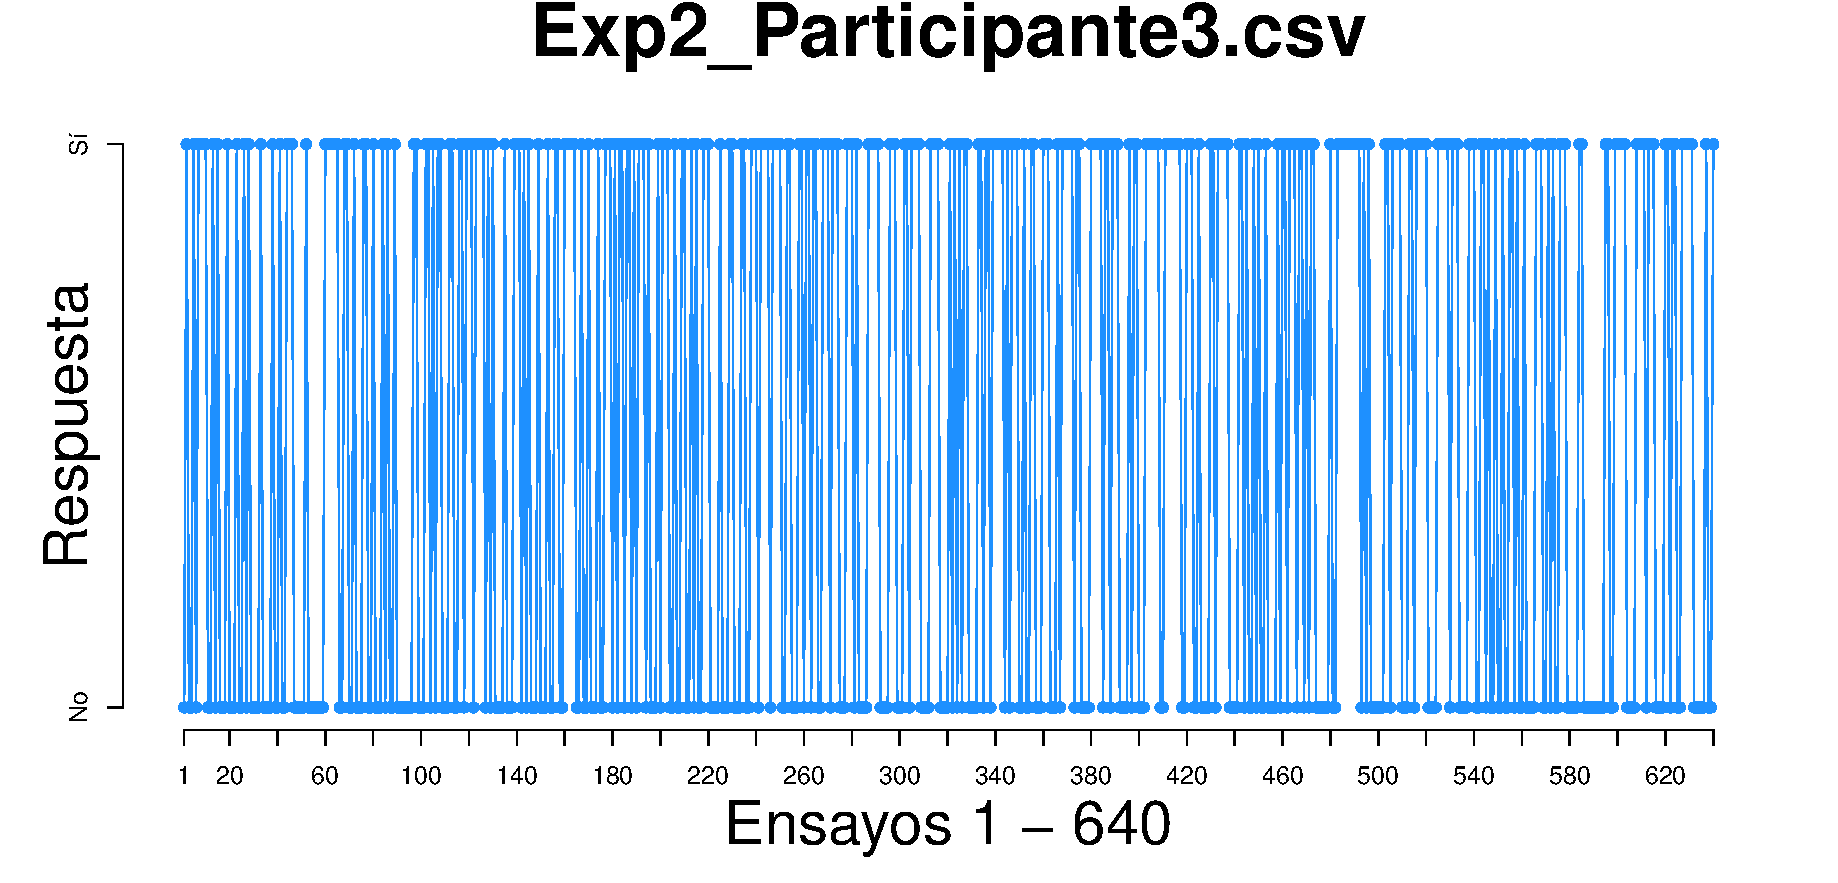
\includegraphics[width=9cm, height=5cm]{Figures/Response_Exp2_P3} 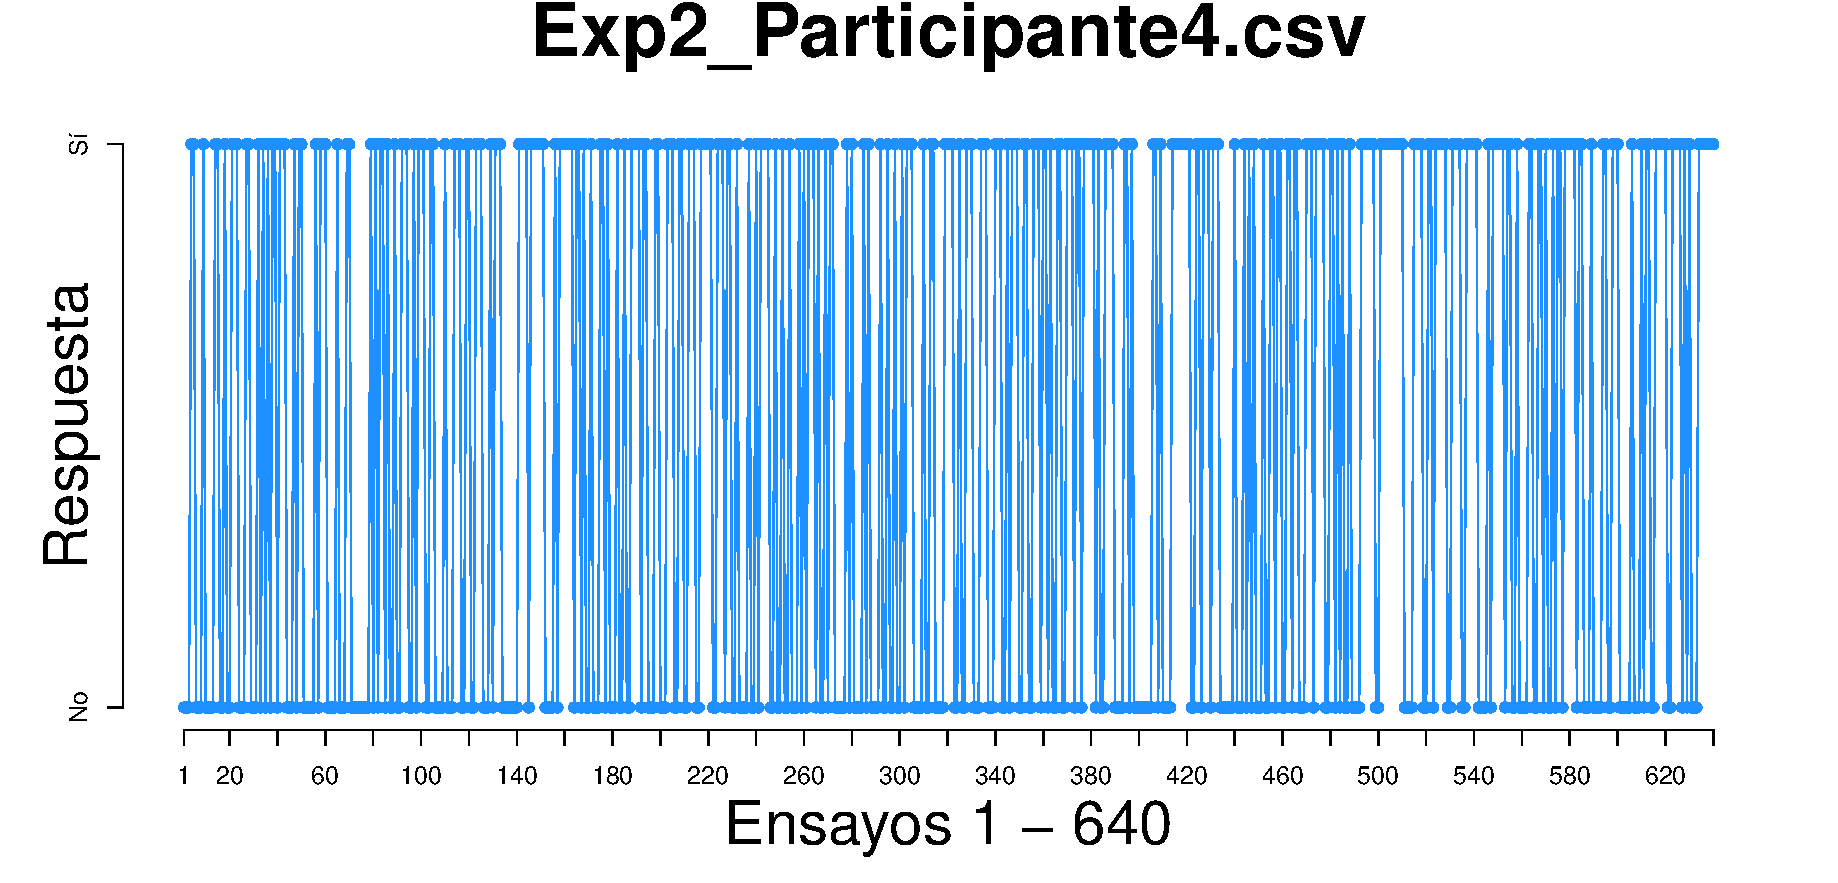
\includegraphics[width=9cm, height=5cm]{Figures/Response_Exp2_P4} 
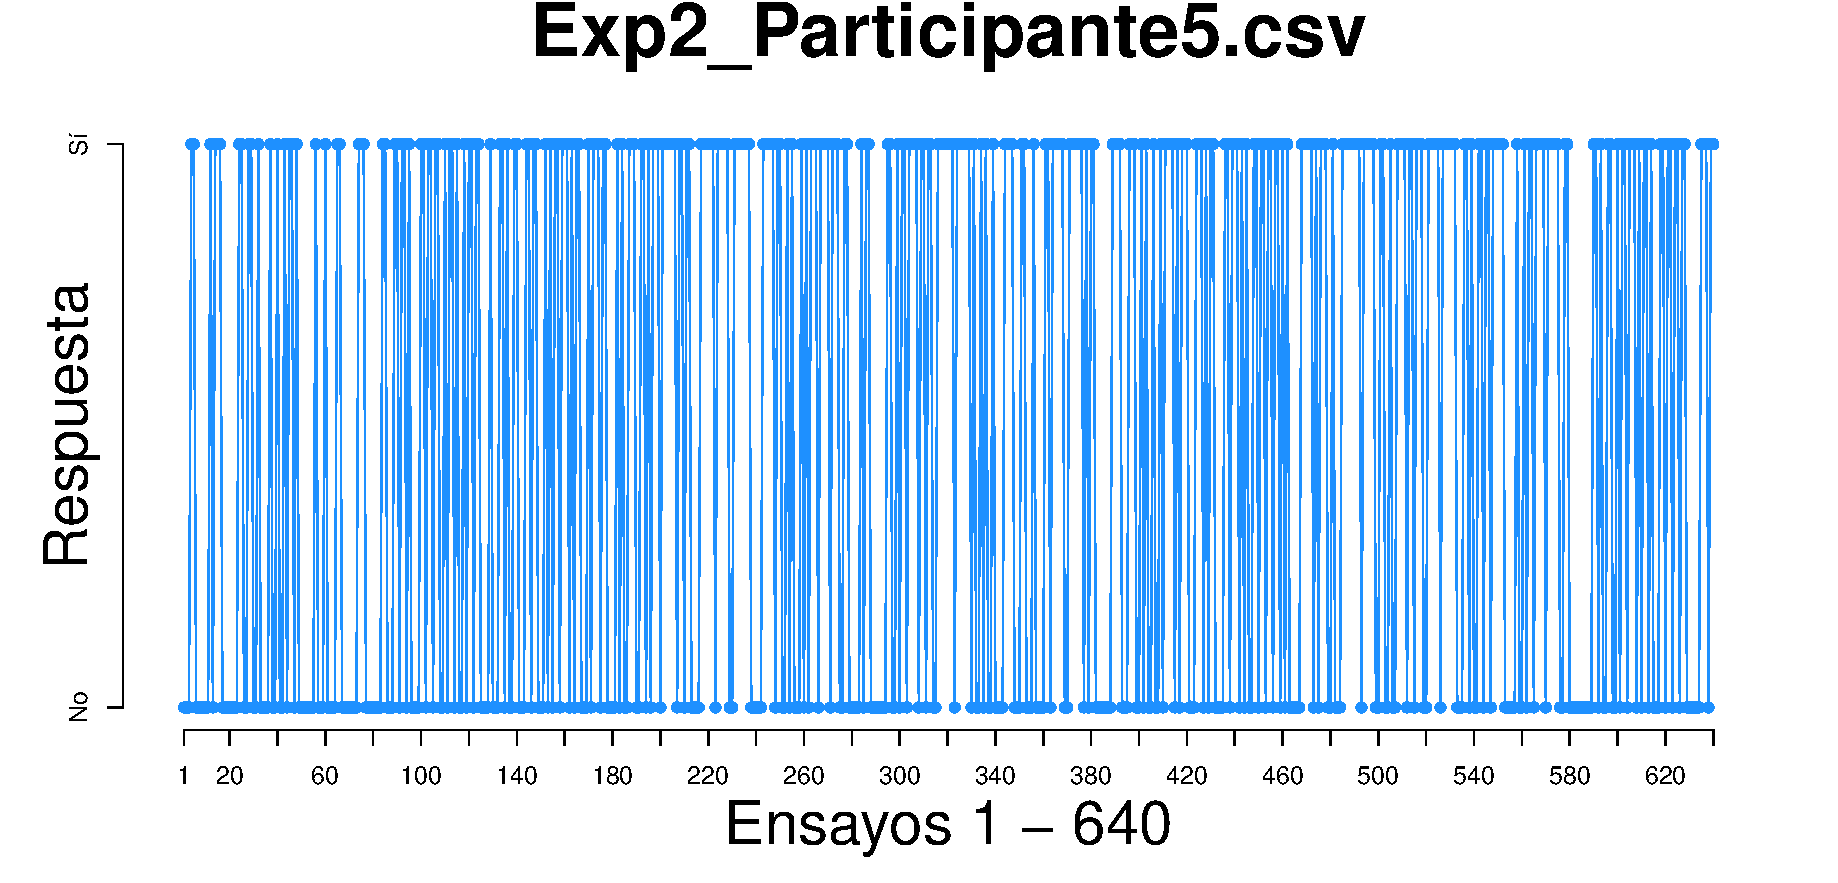
\includegraphics[width=9cm, height=5cm]{Figures/Response_Exp2_P5} 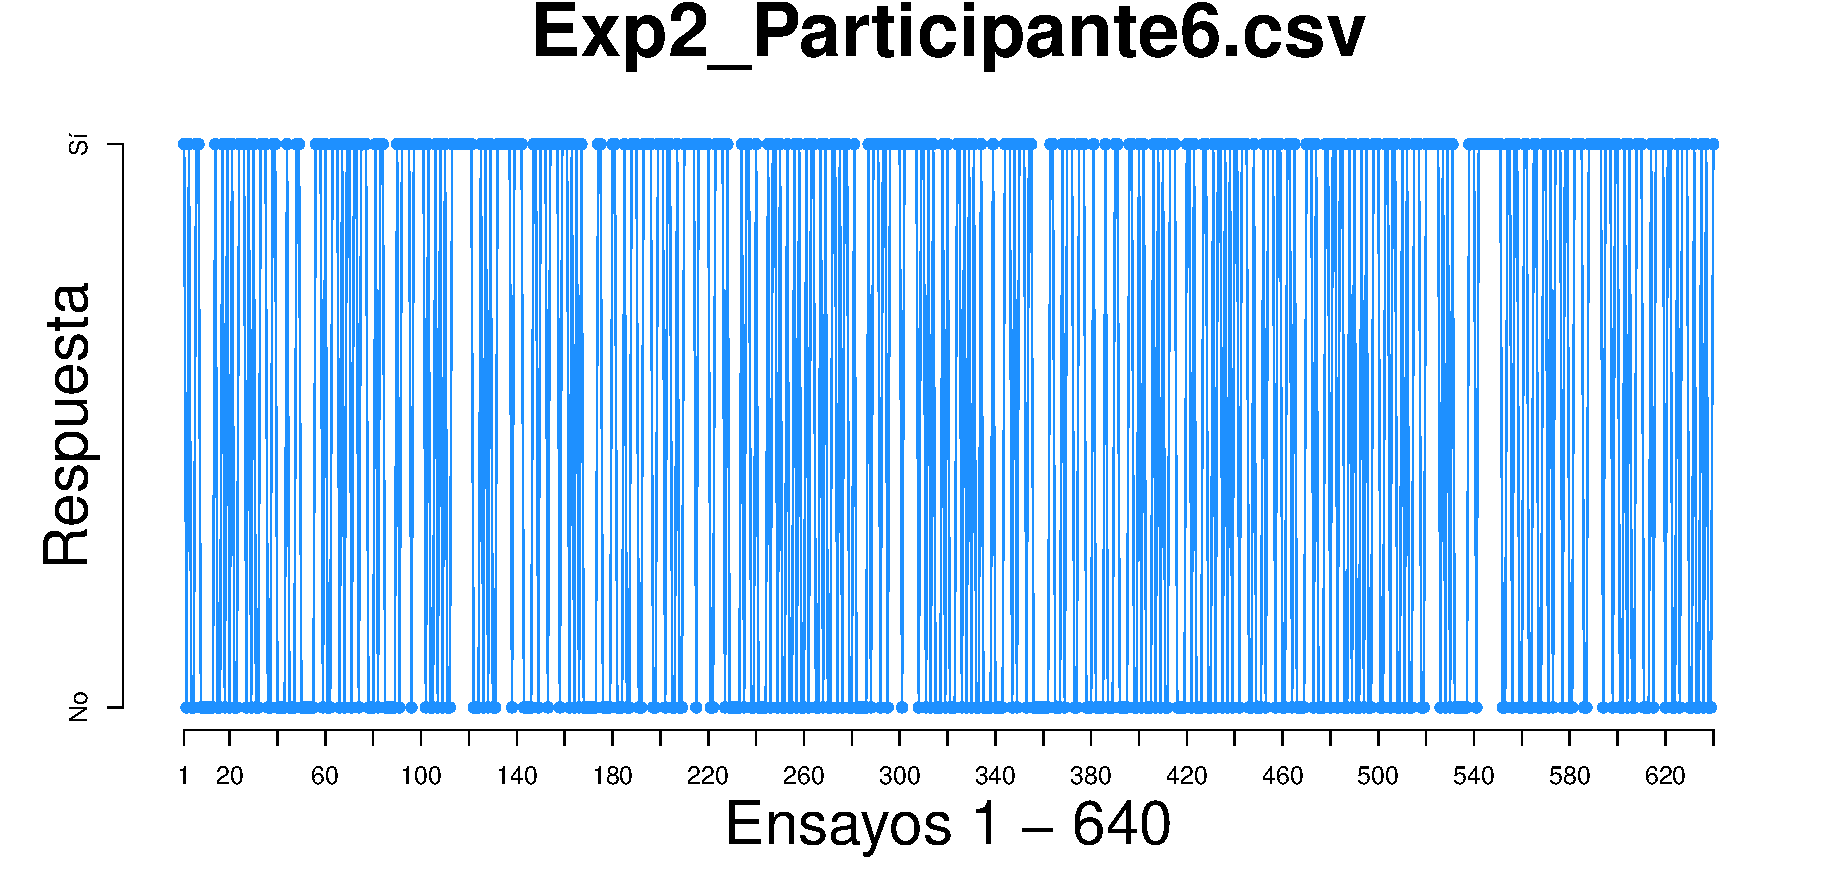
\includegraphics[width=9cm, height=5cm]{Figures/Response_Exp2_P6}
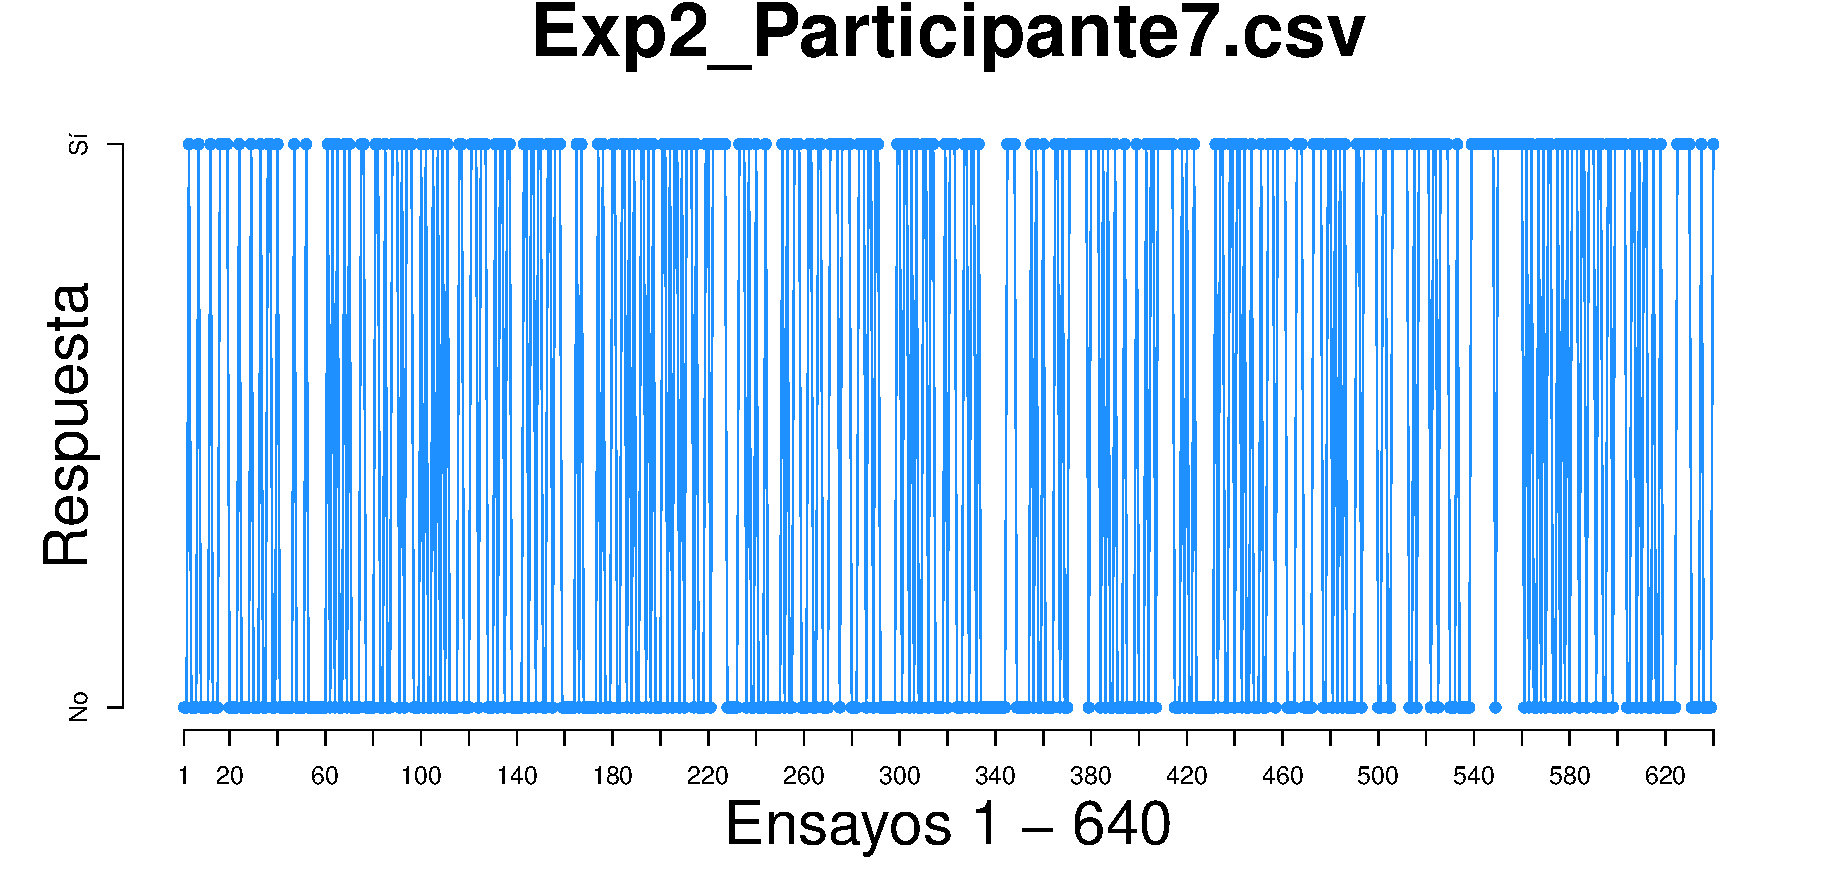
\includegraphics[width=9cm, height=5cm]{Figures/Response_Exp2_P7} 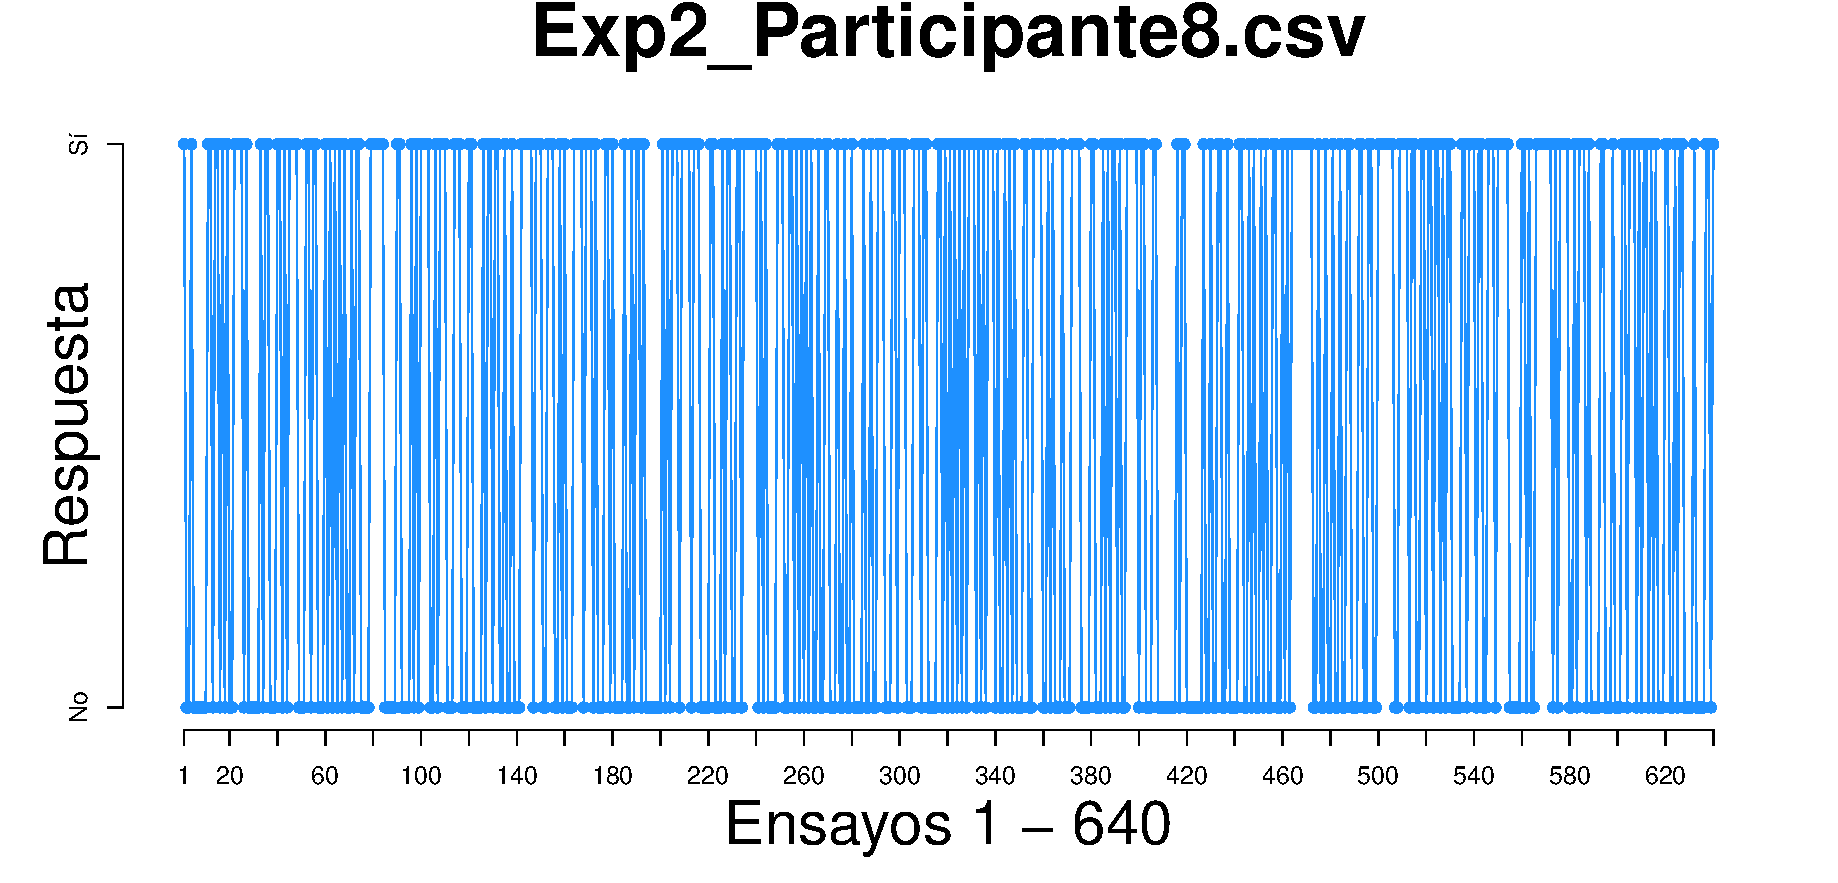
\includegraphics[width=9cm, height=5cm]{Figures/Response_Exp2_P8} 
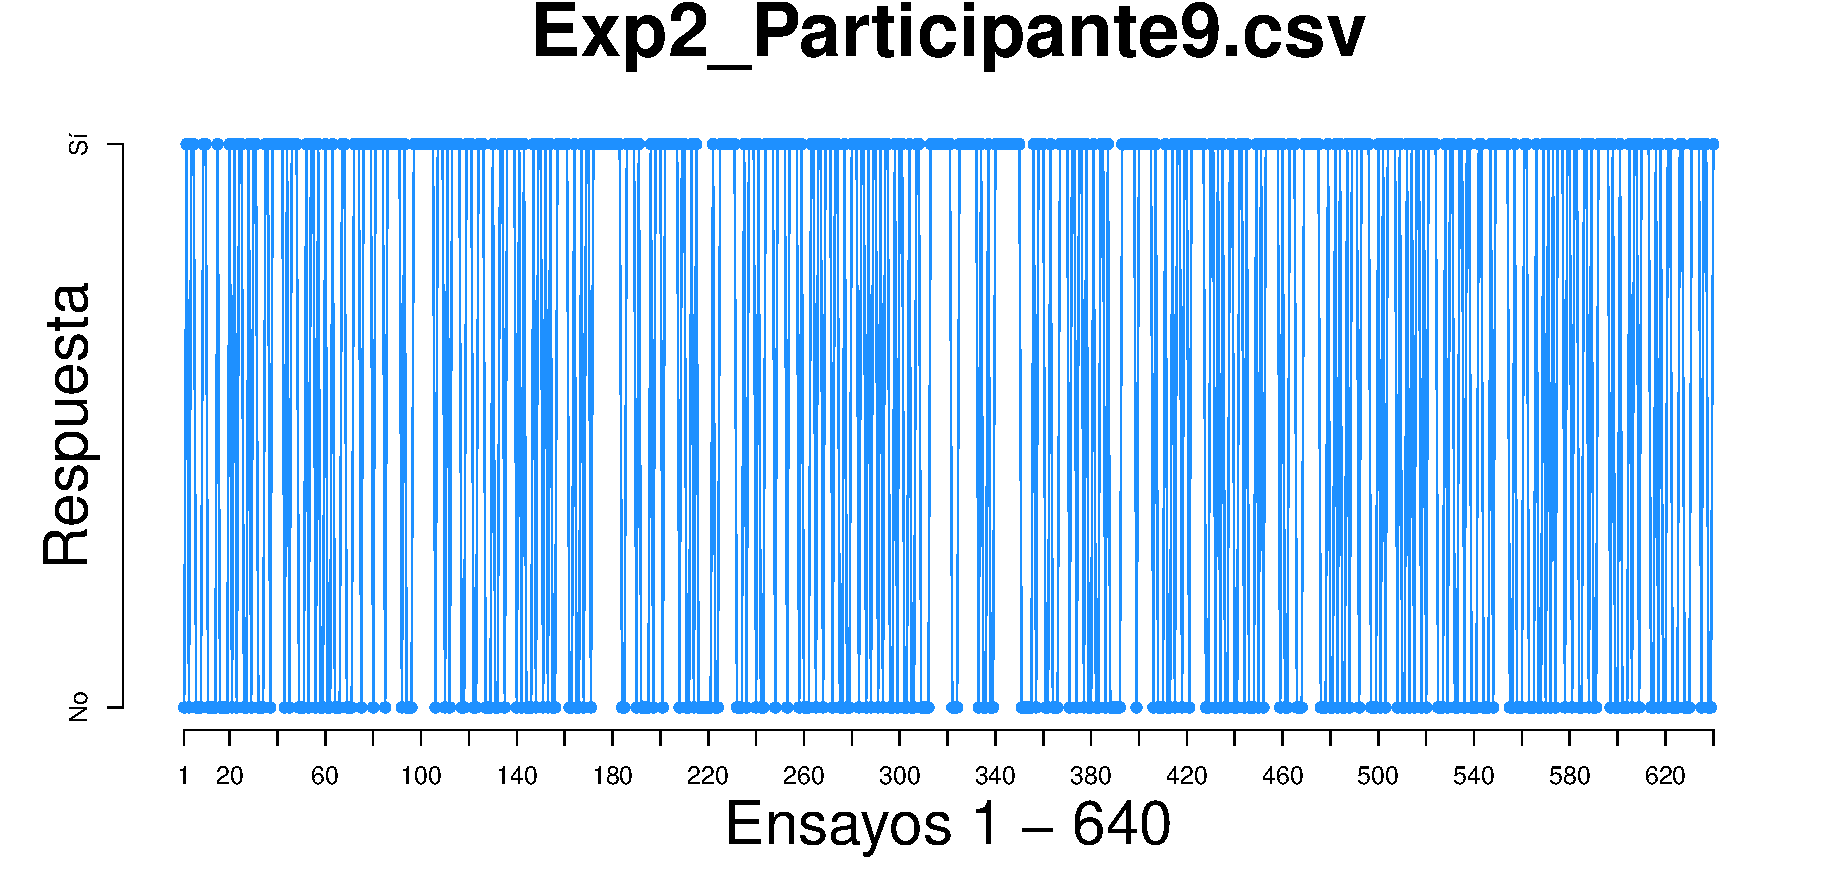
\includegraphics[width=9cm, height=5cm]{Figures/Response_Exp2_P9}
\end{figure}
\vfill .
\begin{figure}[th]
\begin{center}
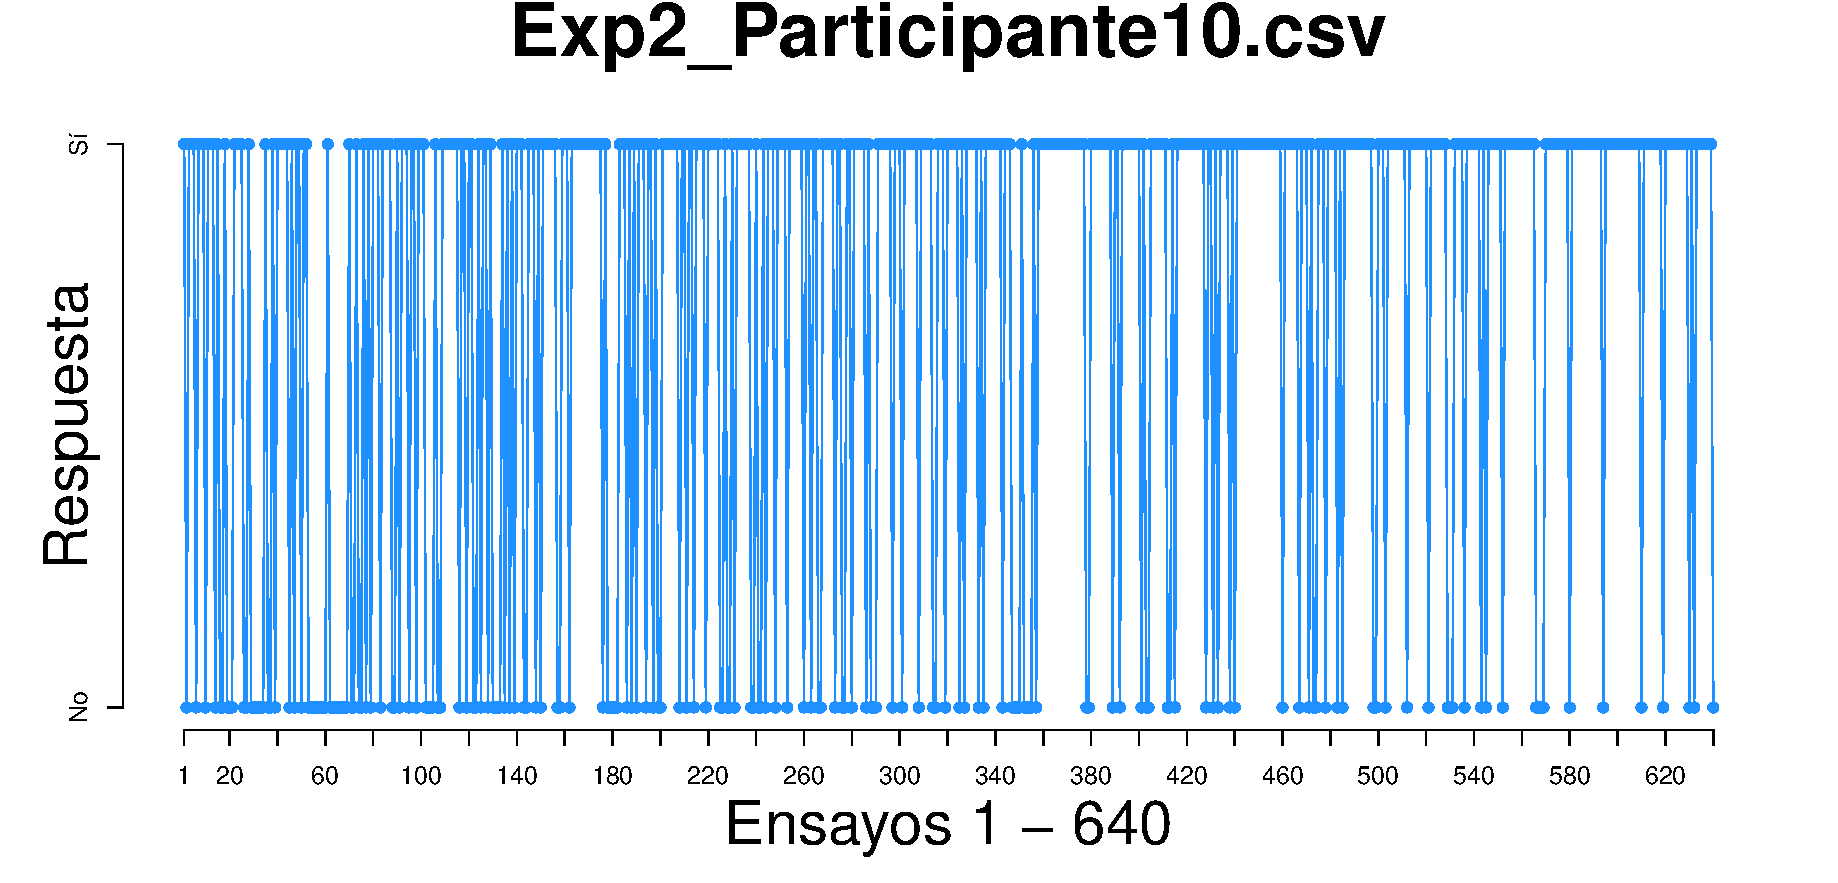
\includegraphics[width=8cm, height=4cm]{Figures/Response_Exp2_P10} 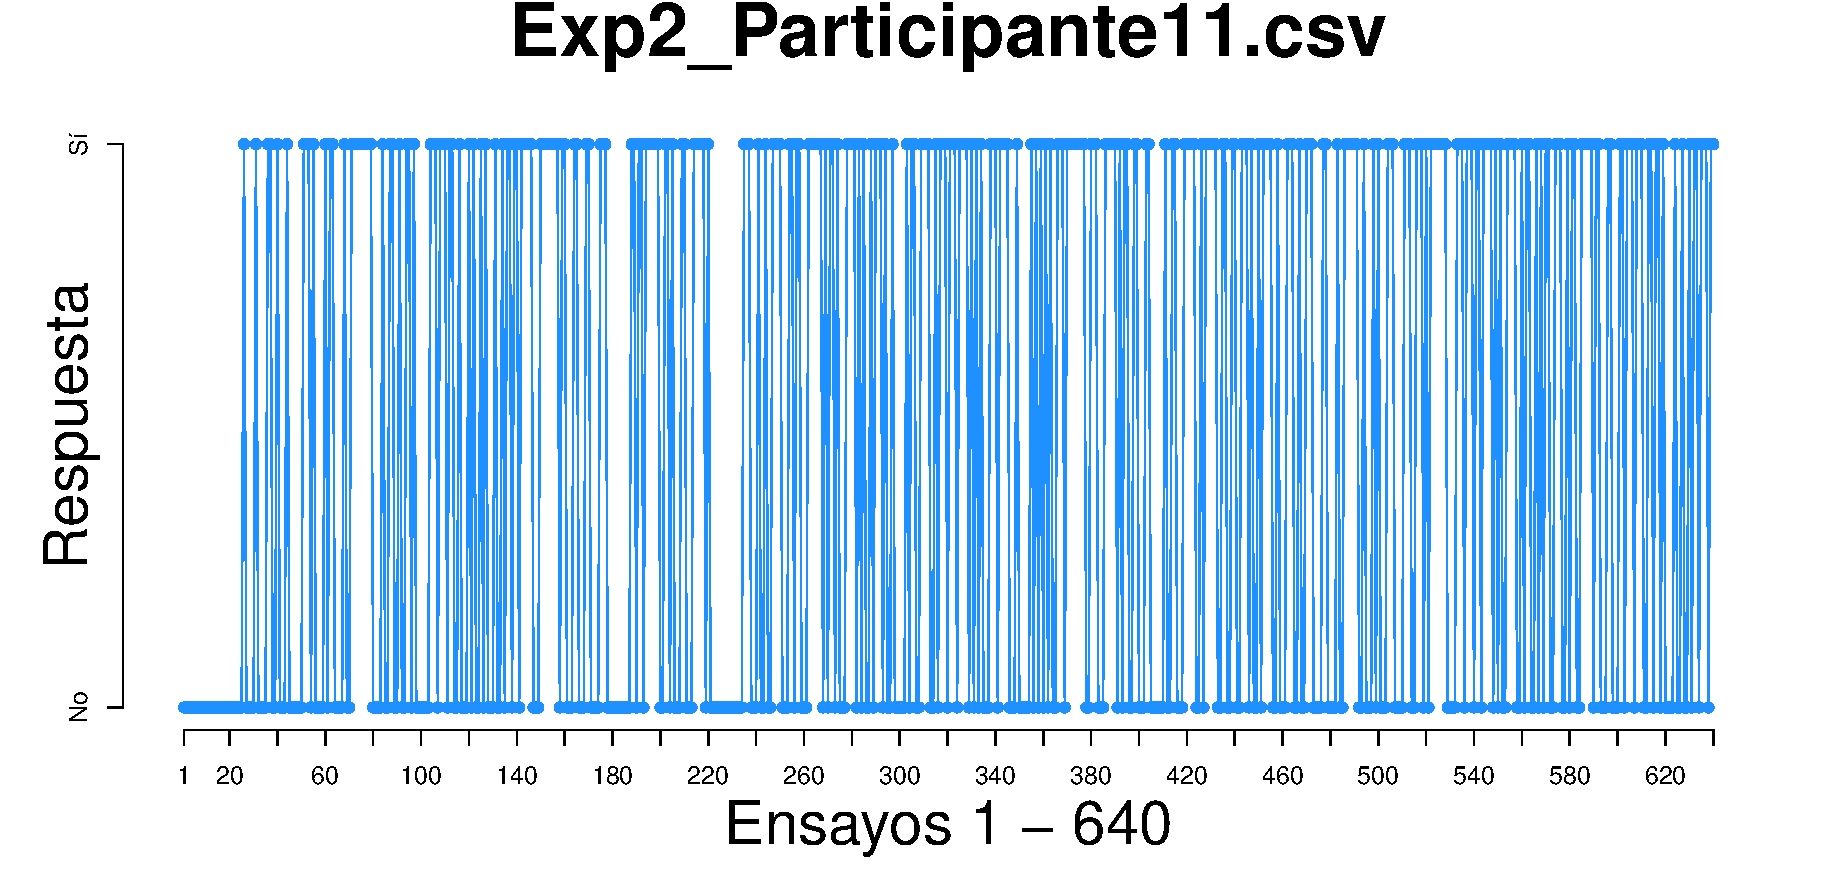
\includegraphics[width=8cm, height=4cm]{Figures/Response_Exp2_P11} 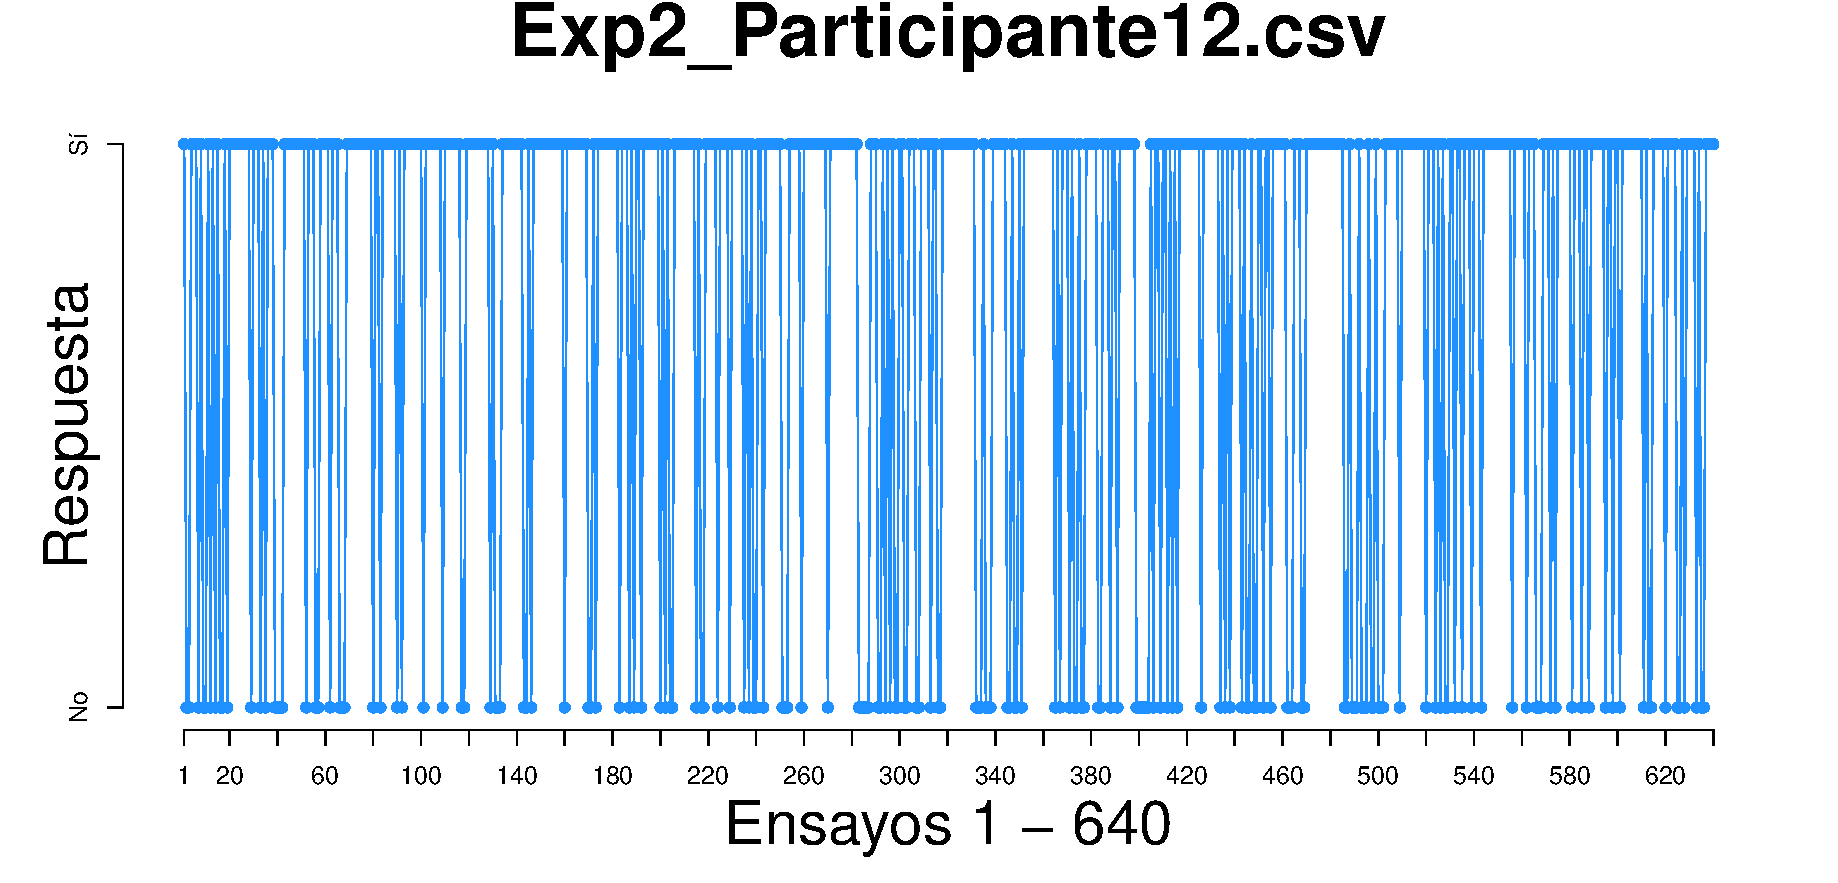
\includegraphics[width=8cm, height=4cm]{Figures/Response_Exp2_P12}
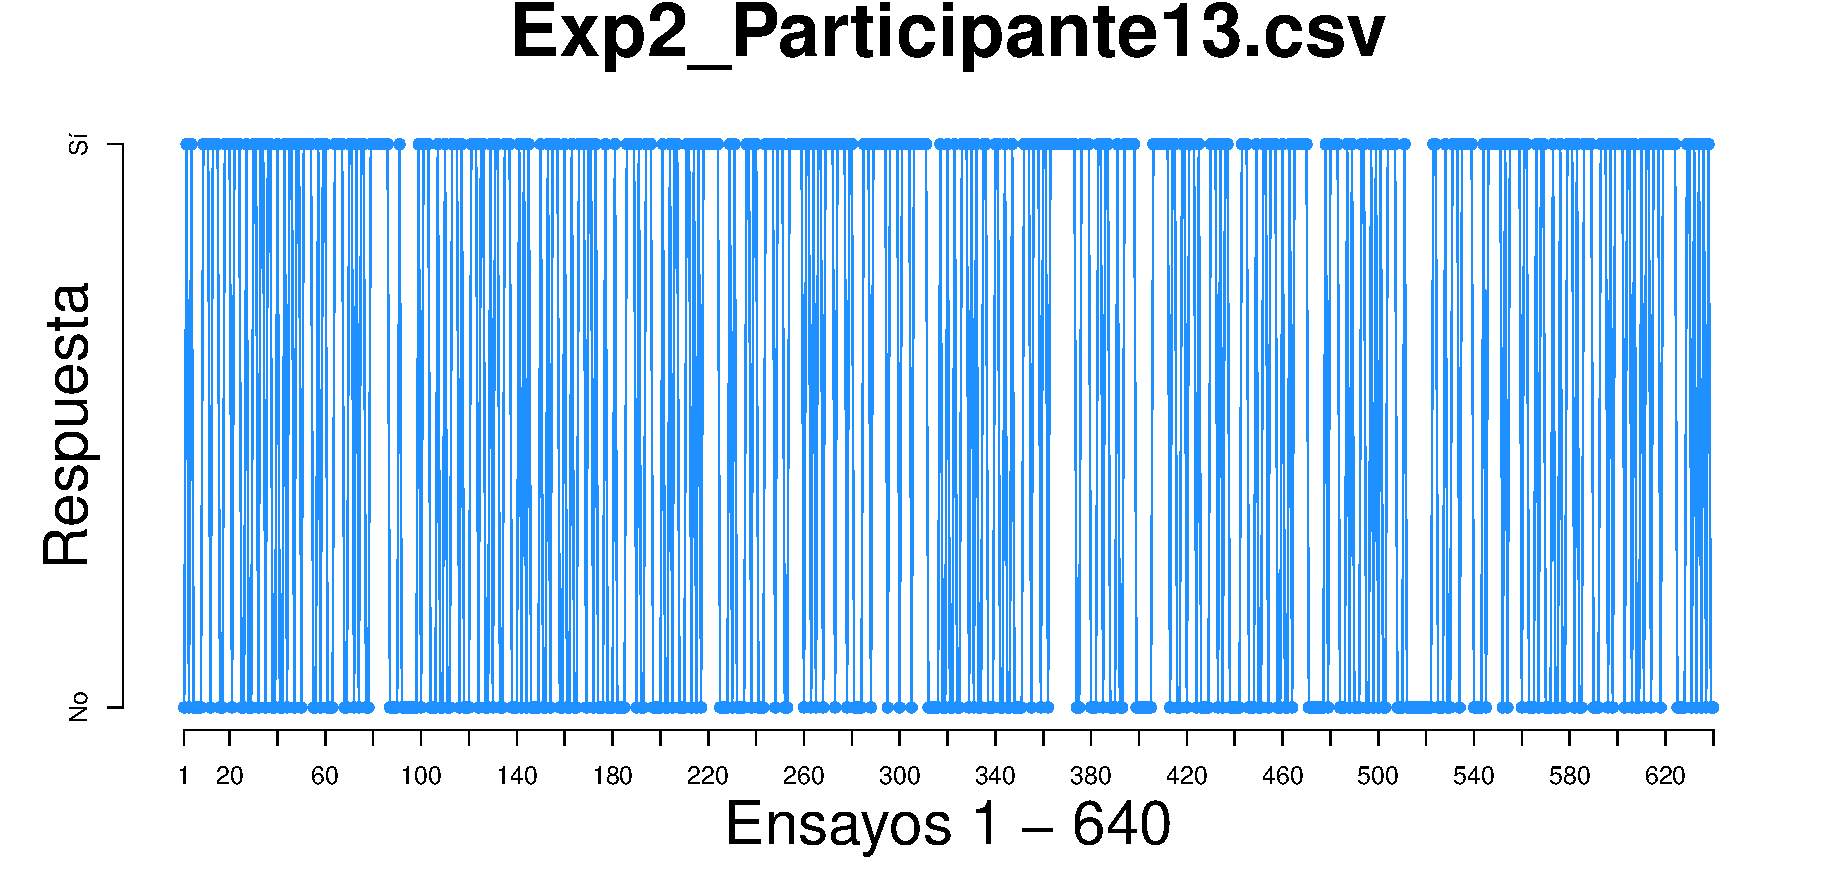
\includegraphics[width=8cm, height=4cm]{Figures/Response_Exp2_P13} 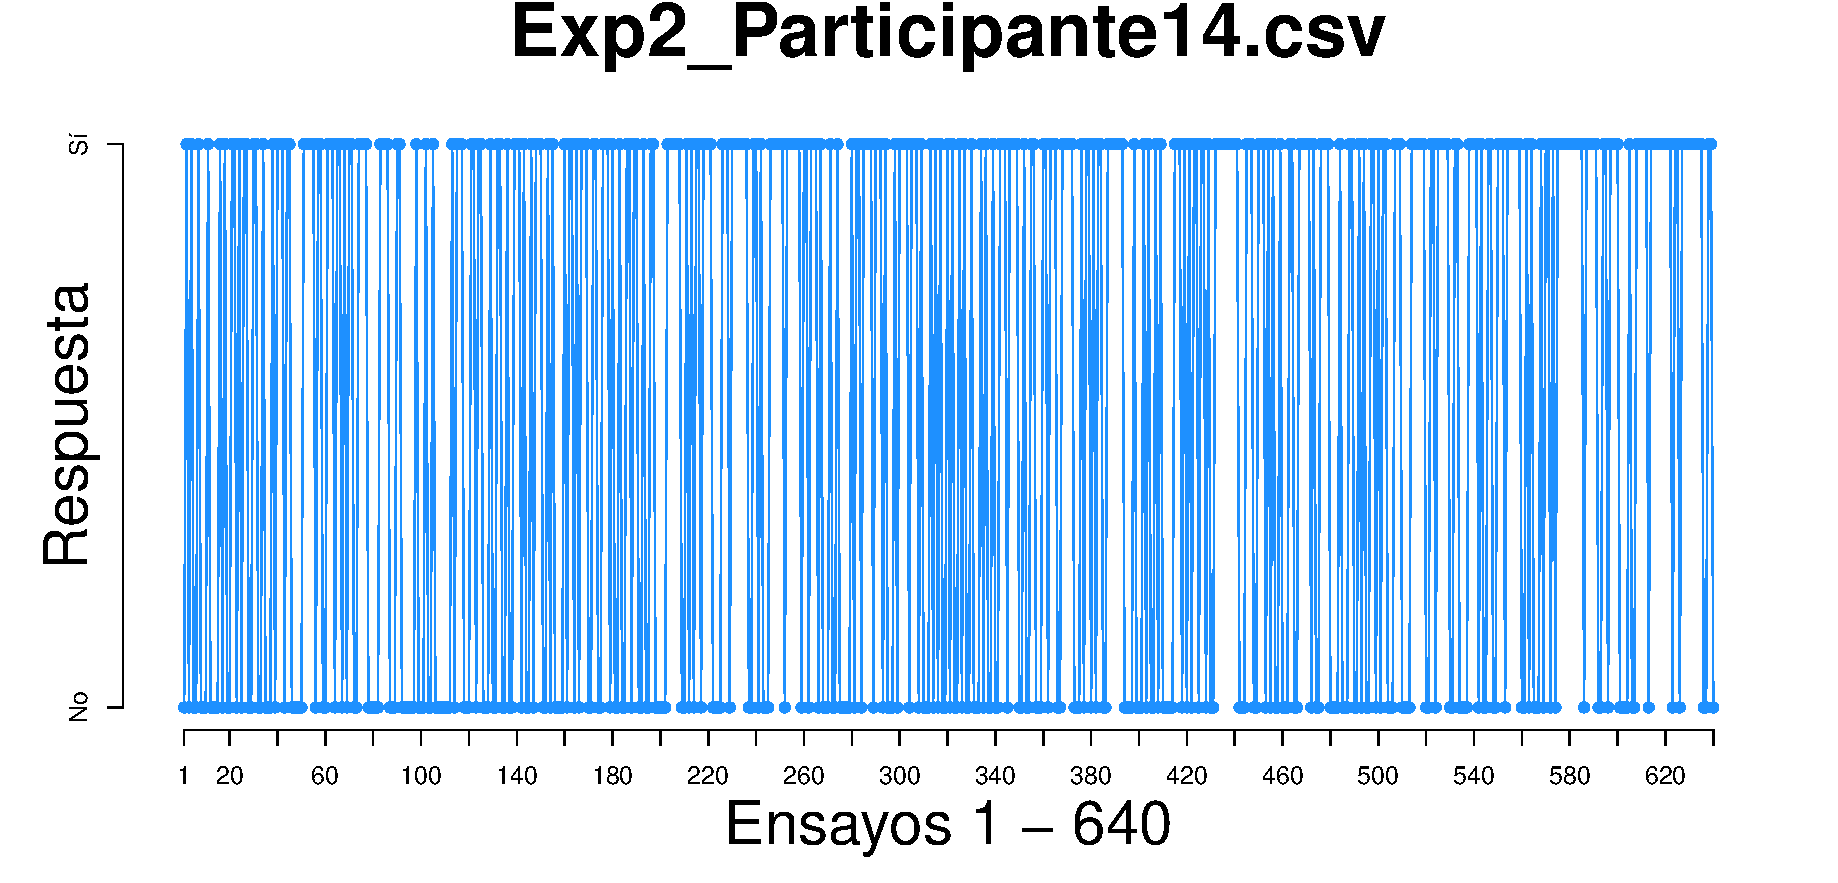
\includegraphics[width=8cm, height=4cm]{Figures/Response_Exp2_P14} 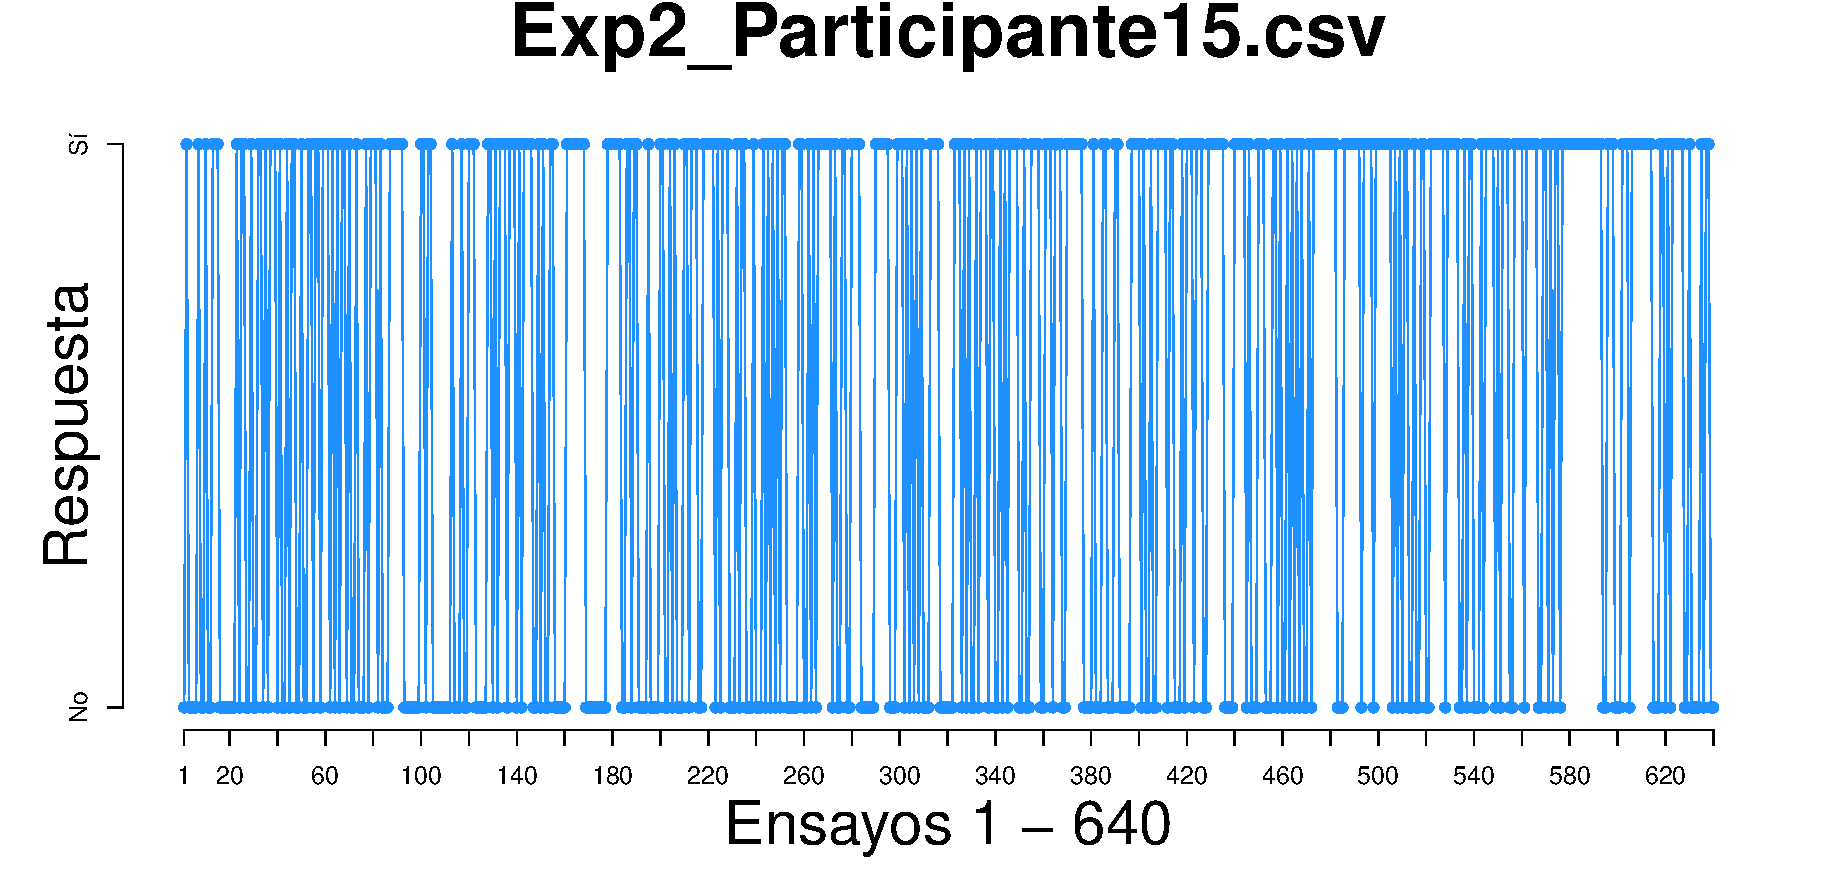
\includegraphics[width=8cm, height=4cm]{Figures/Response_Exp2_P15}
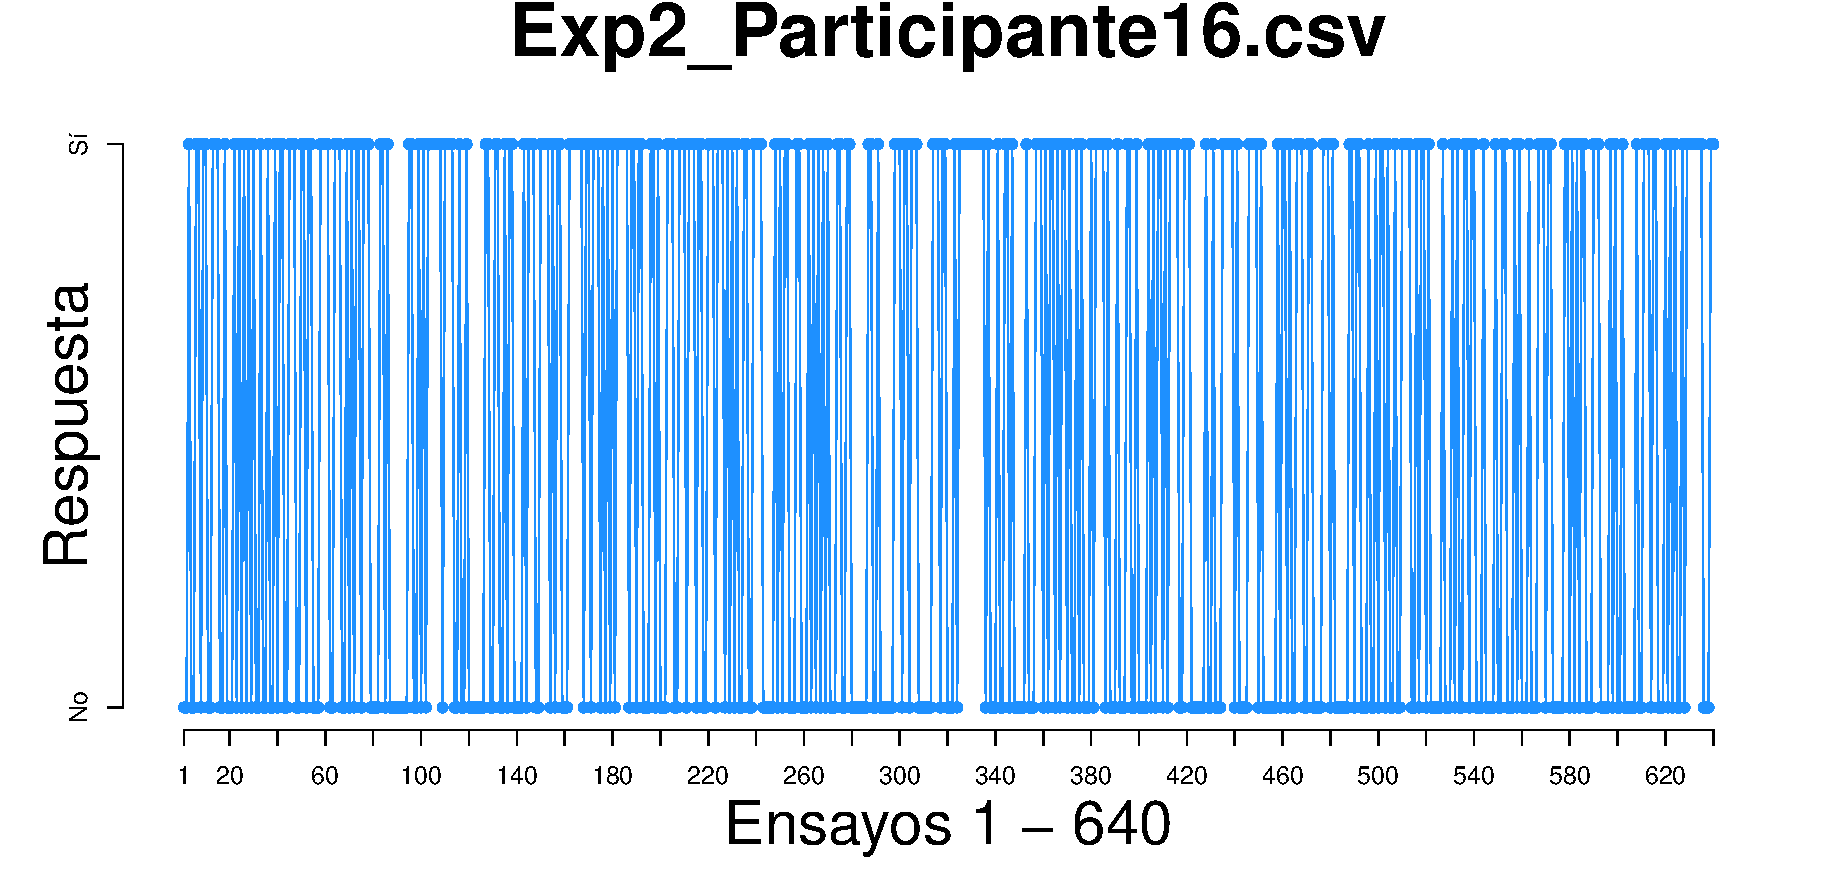
\includegraphics[width=8cm, height=4cm]{Figures/Response_Exp2_P16} 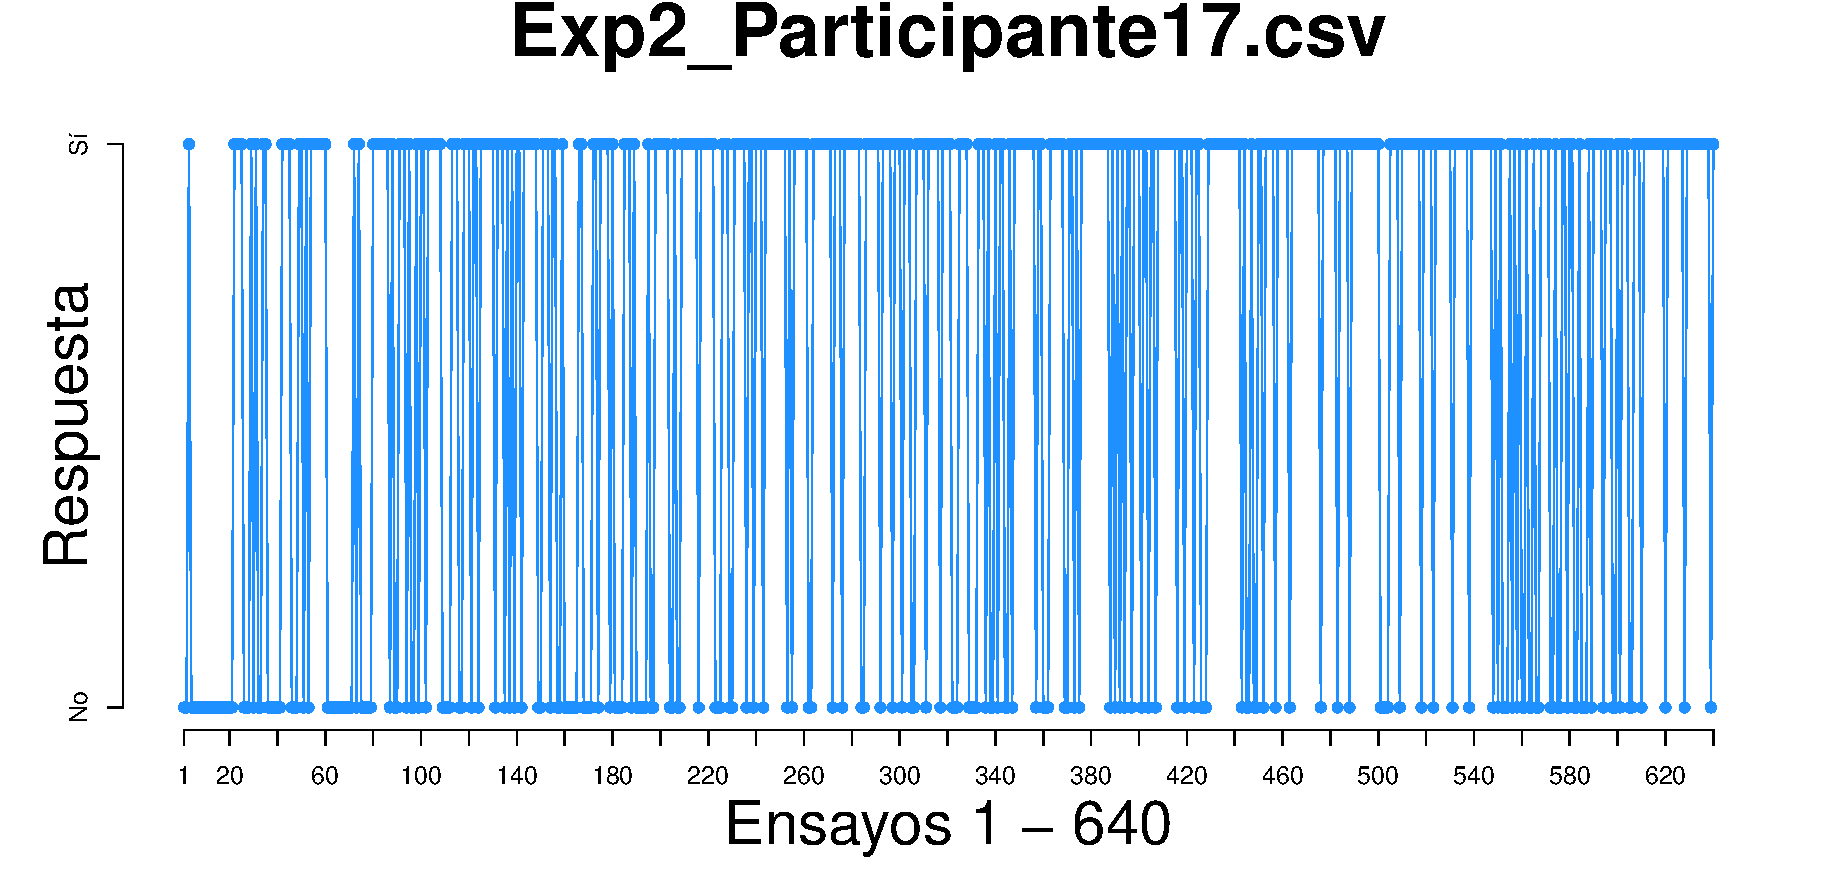
\includegraphics[width=8cm, height=4cm]{Figures/Response_Exp2_P17} 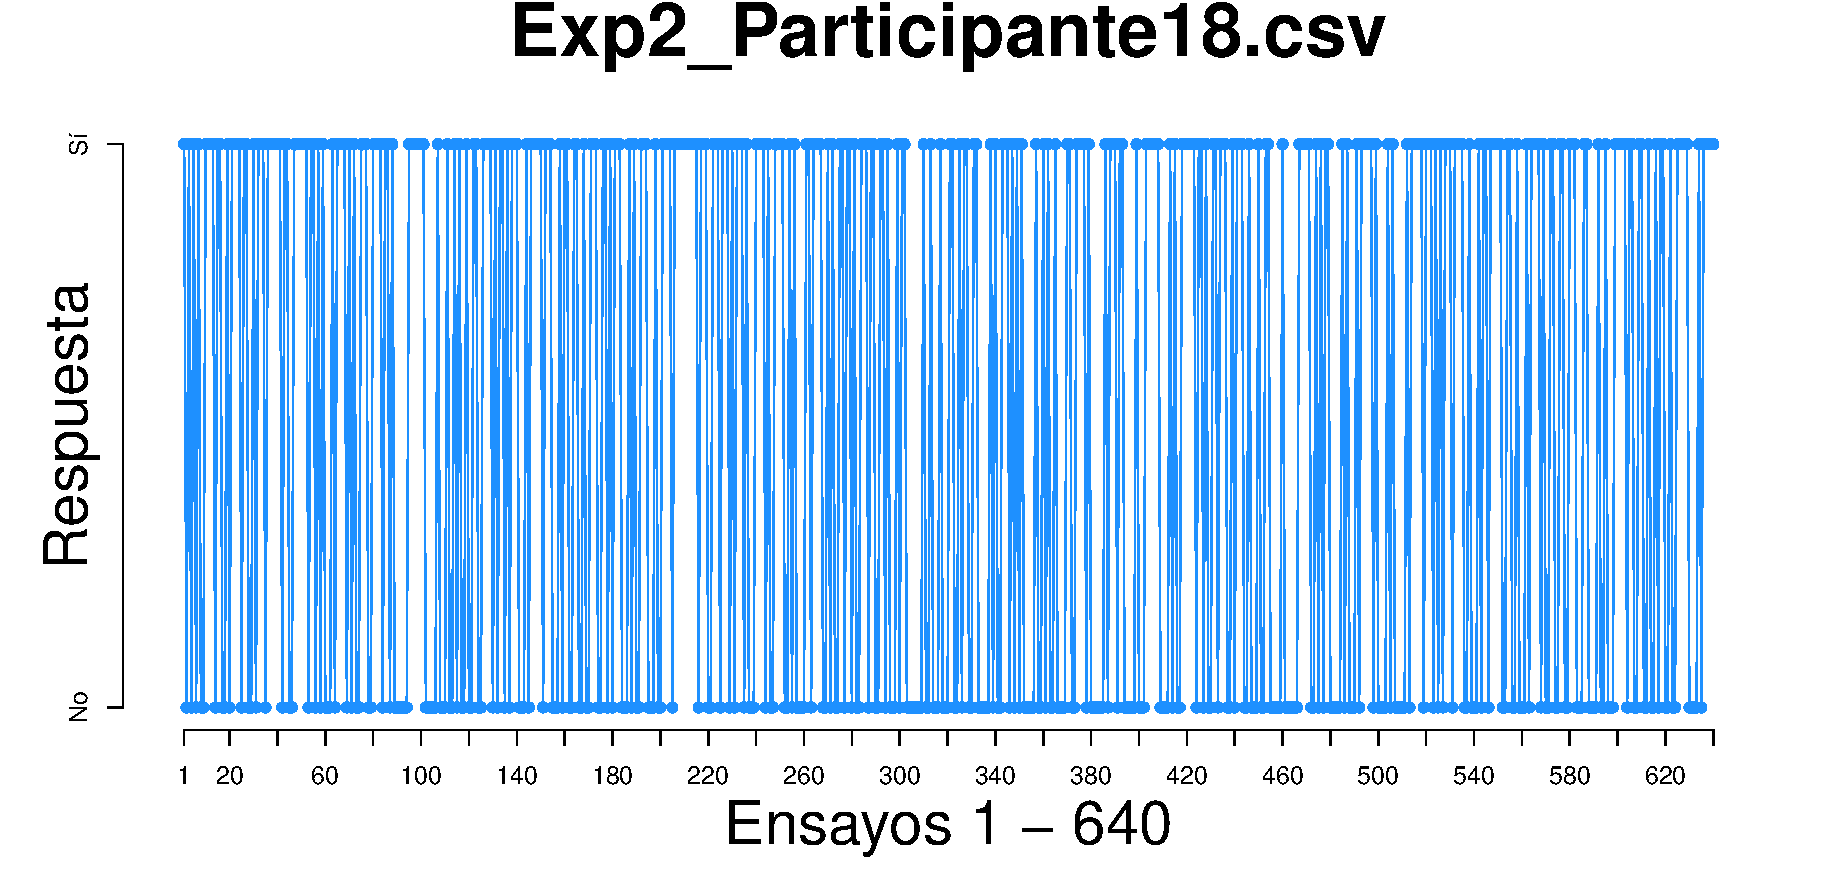
\includegraphics[width=8cm, height=4cm]{Figures/Response_Exp2_P18}
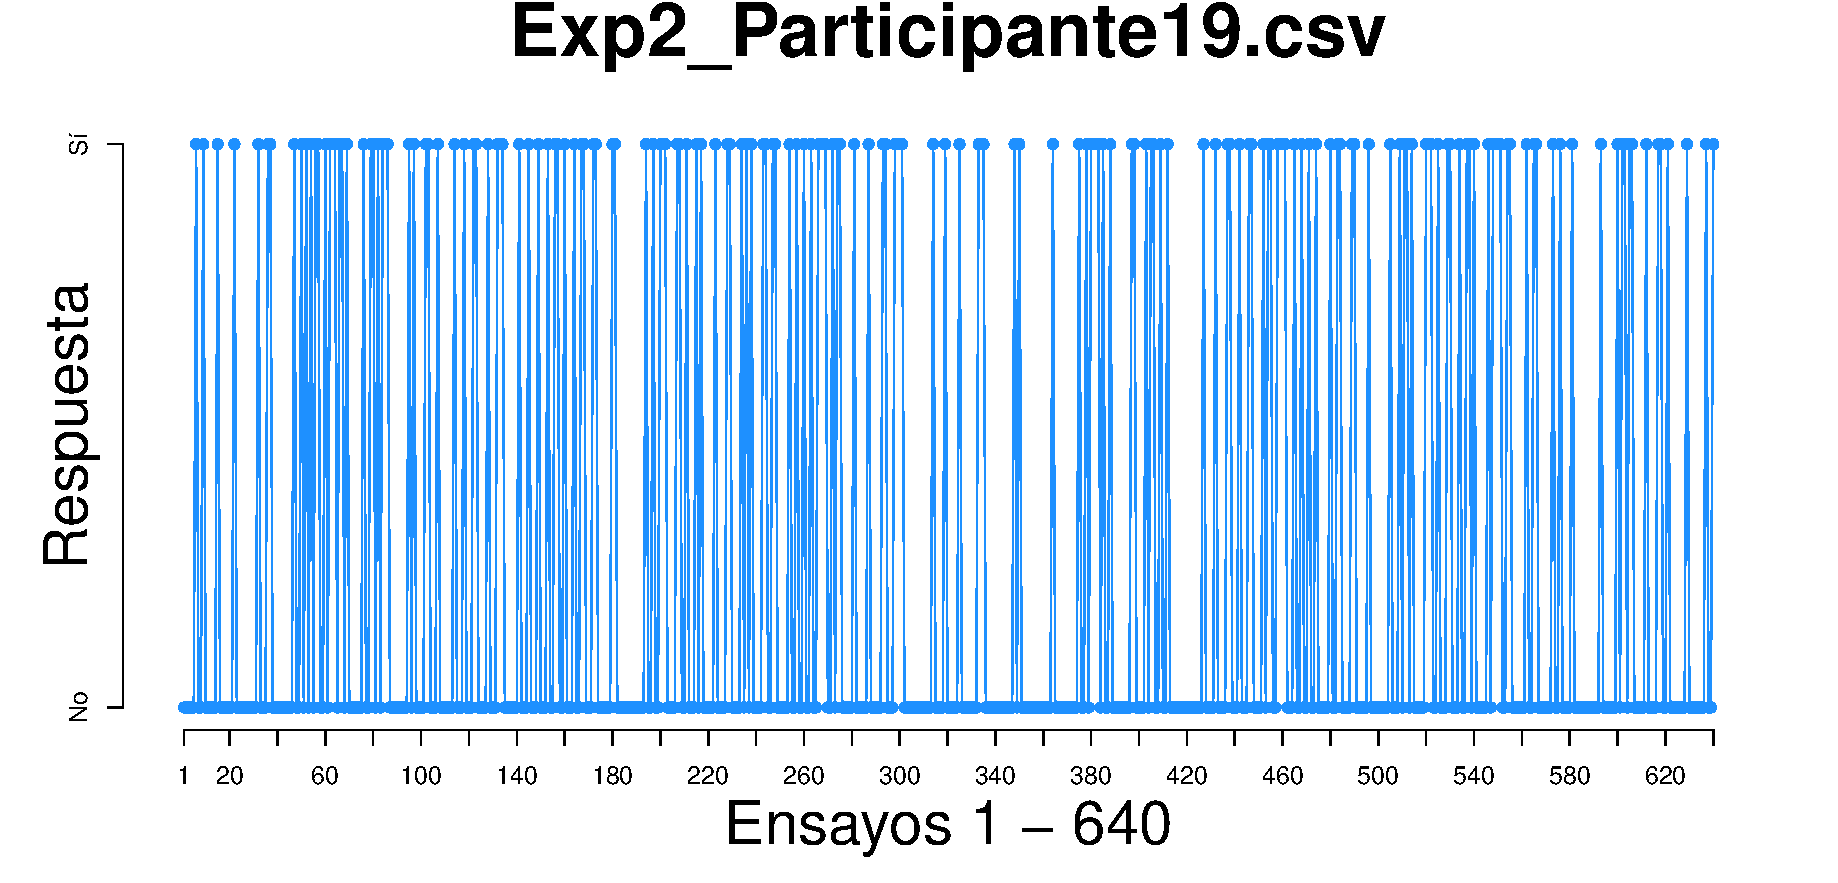
\includegraphics[width=8cm, height=4cm]{Figures/Response_Exp2_P19} 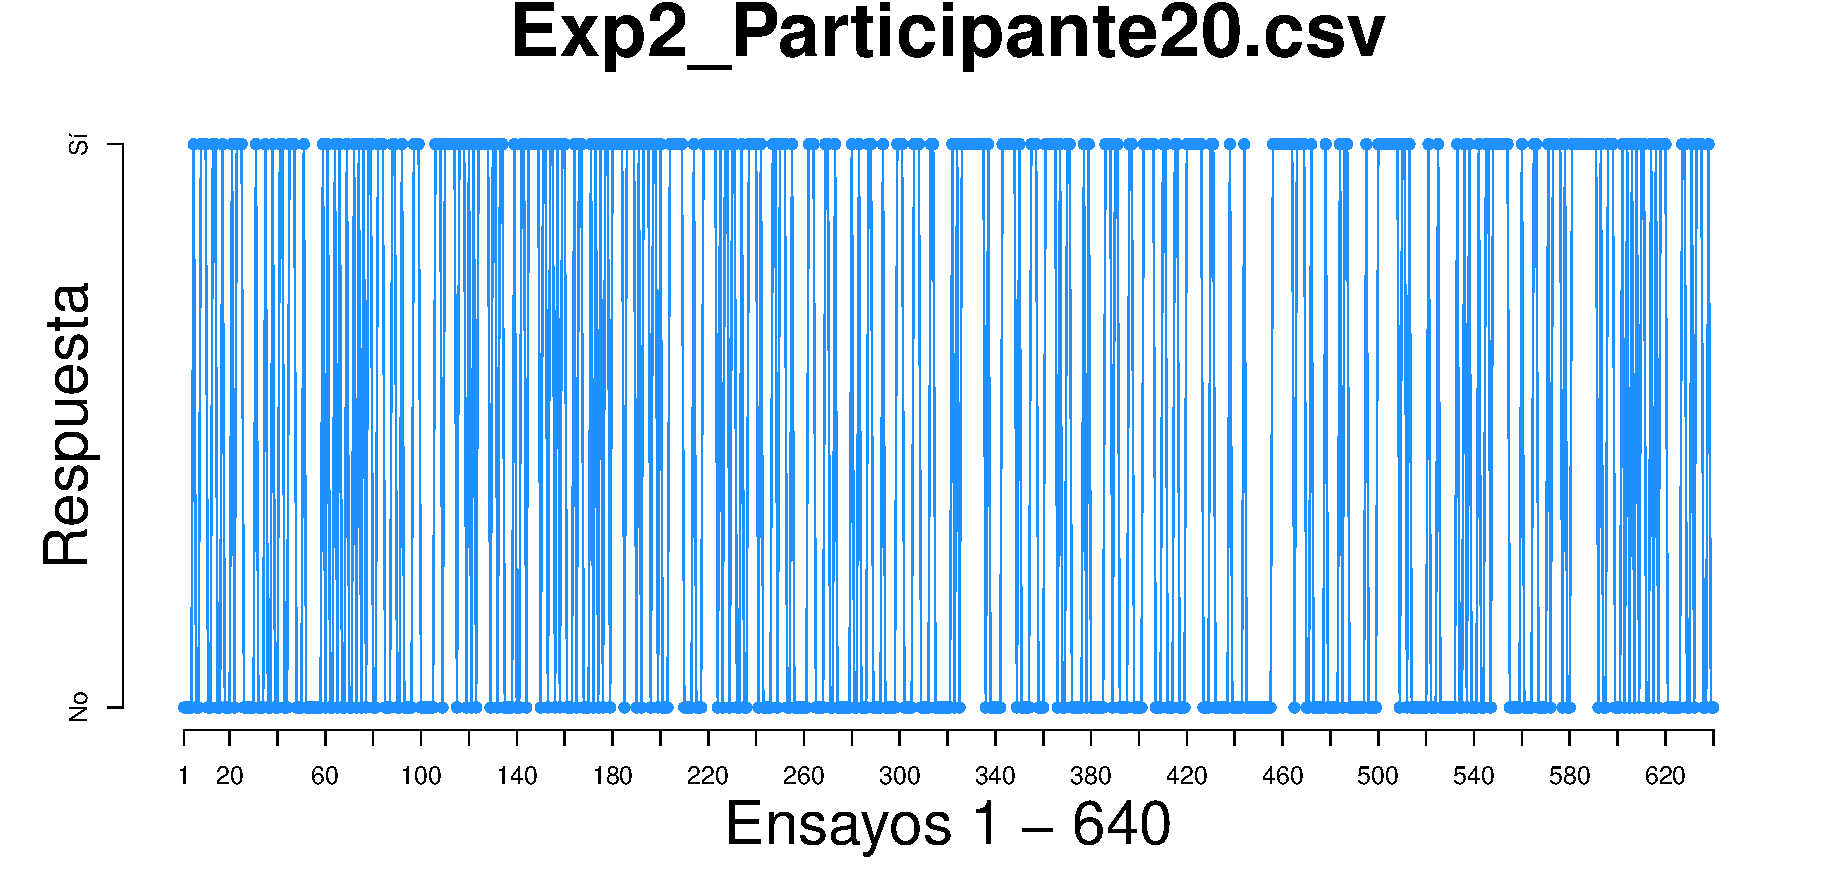
\includegraphics[width=8cm, height=4cm]{Figures/Response_Exp2_P20} 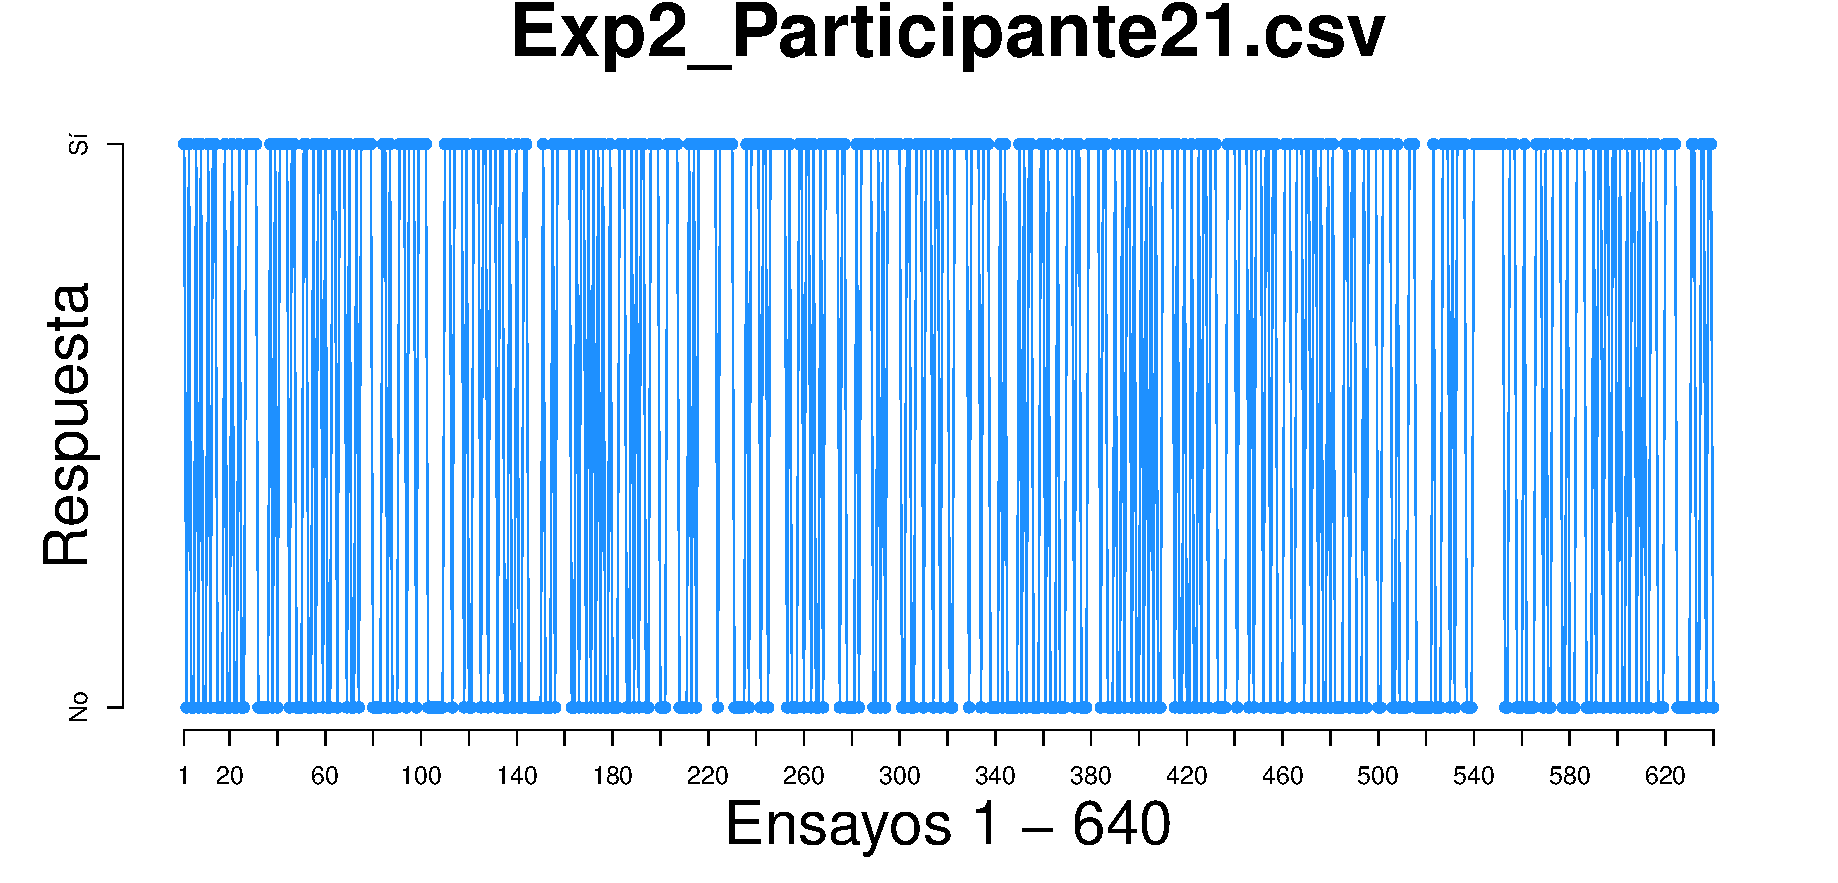
\includegraphics[width=8cm, height=4cm]{Figures/Response_Exp2_P21} 
\end{center}
\end{figure}
\clearpage










---
\vspace{3mm}
\begin{center}
{\LARGE \textbf{Correlación entre la Respuesta binaria registrada y el tipo de ensayo}}\\
{\small \textsc{(evaluando sesgos evidentes)}}\\
\smallskip
\end{center}
\begin{center}
{\LARGE \textit{Experimento 1}}\\
\end{center}
\vspace{3mm}
\begin{figure}[th]
\centering
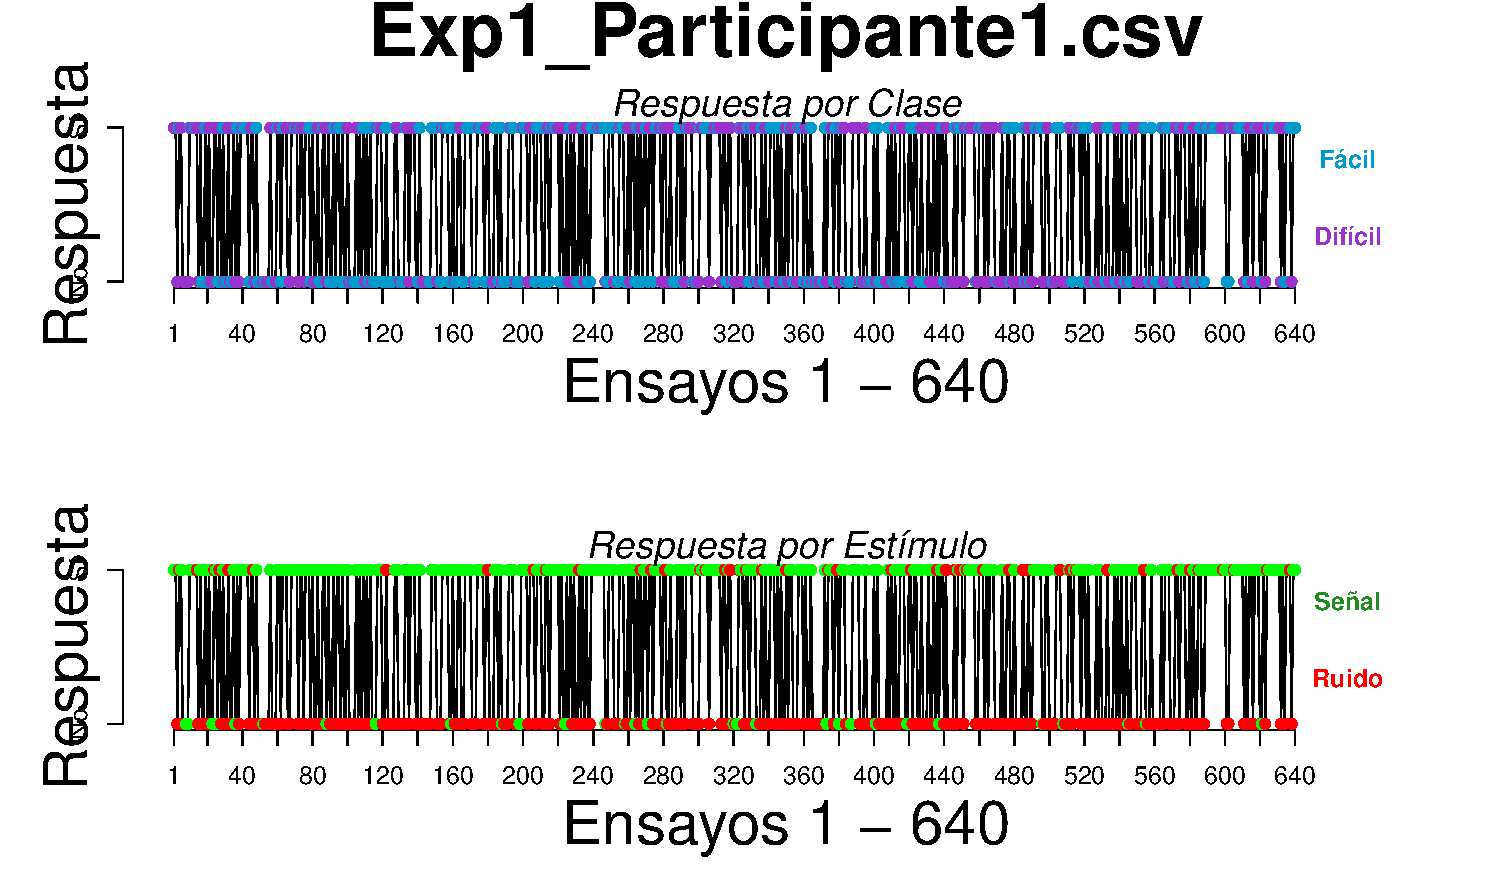
\includegraphics[width=9cm, height=5cm]{Figures/BiasResp_Exp1_P1} 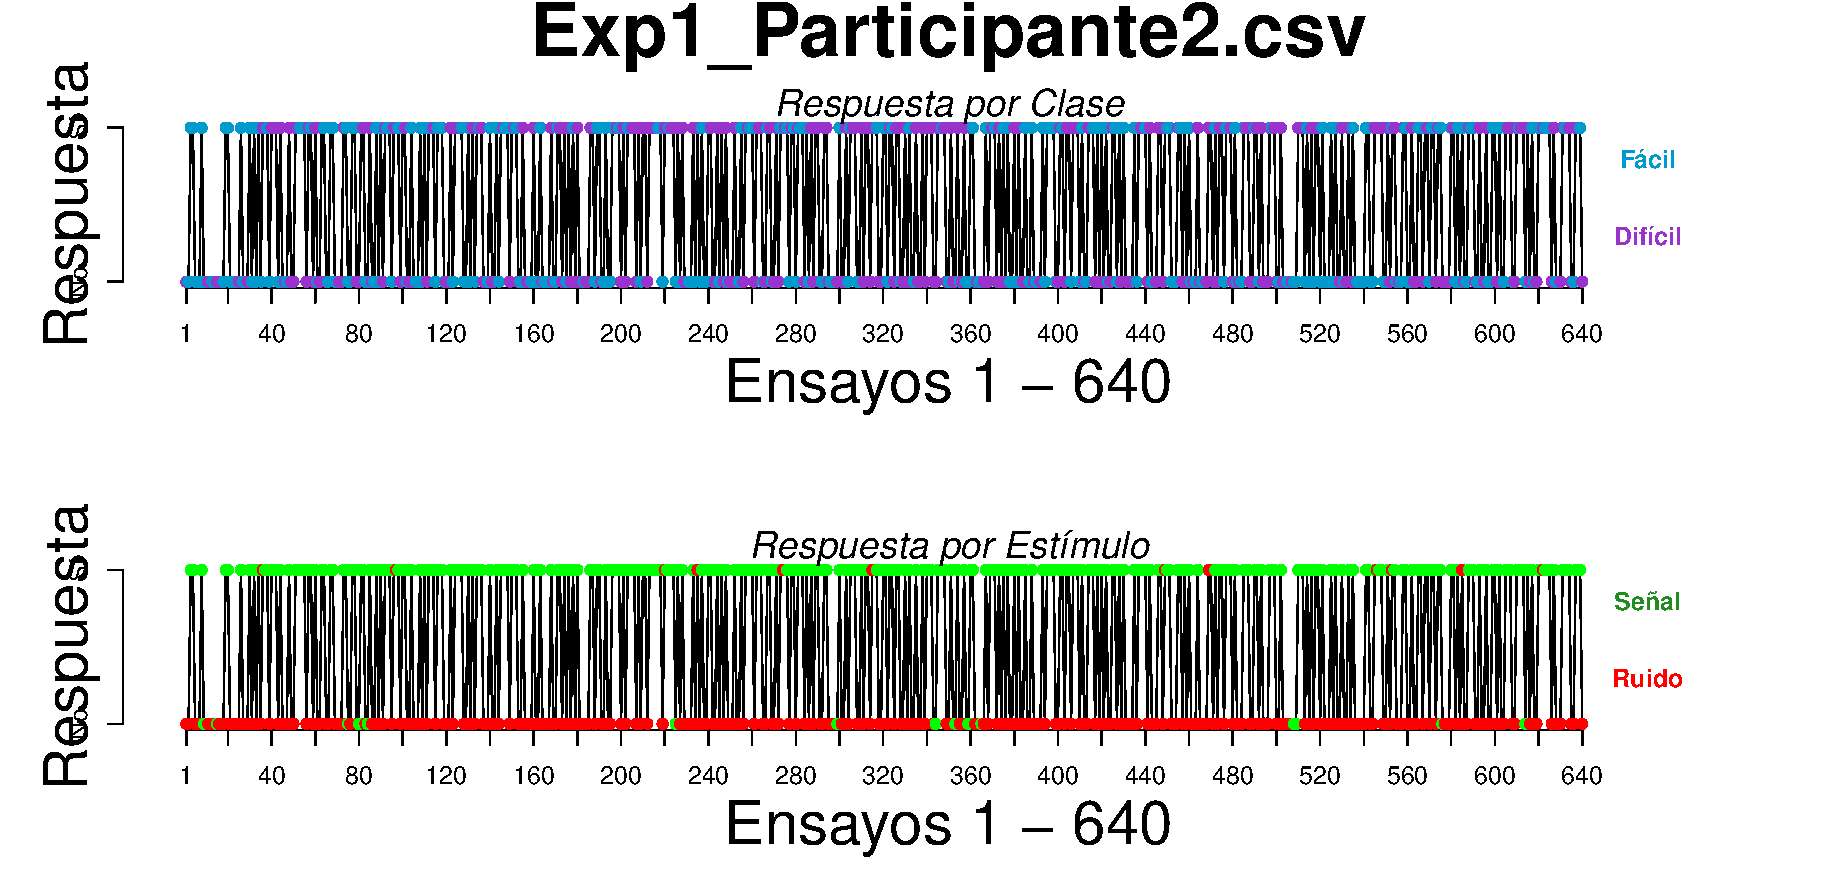
\includegraphics[width=9cm, height=5cm]{Figures/BiasResp_Exp1_P2} 
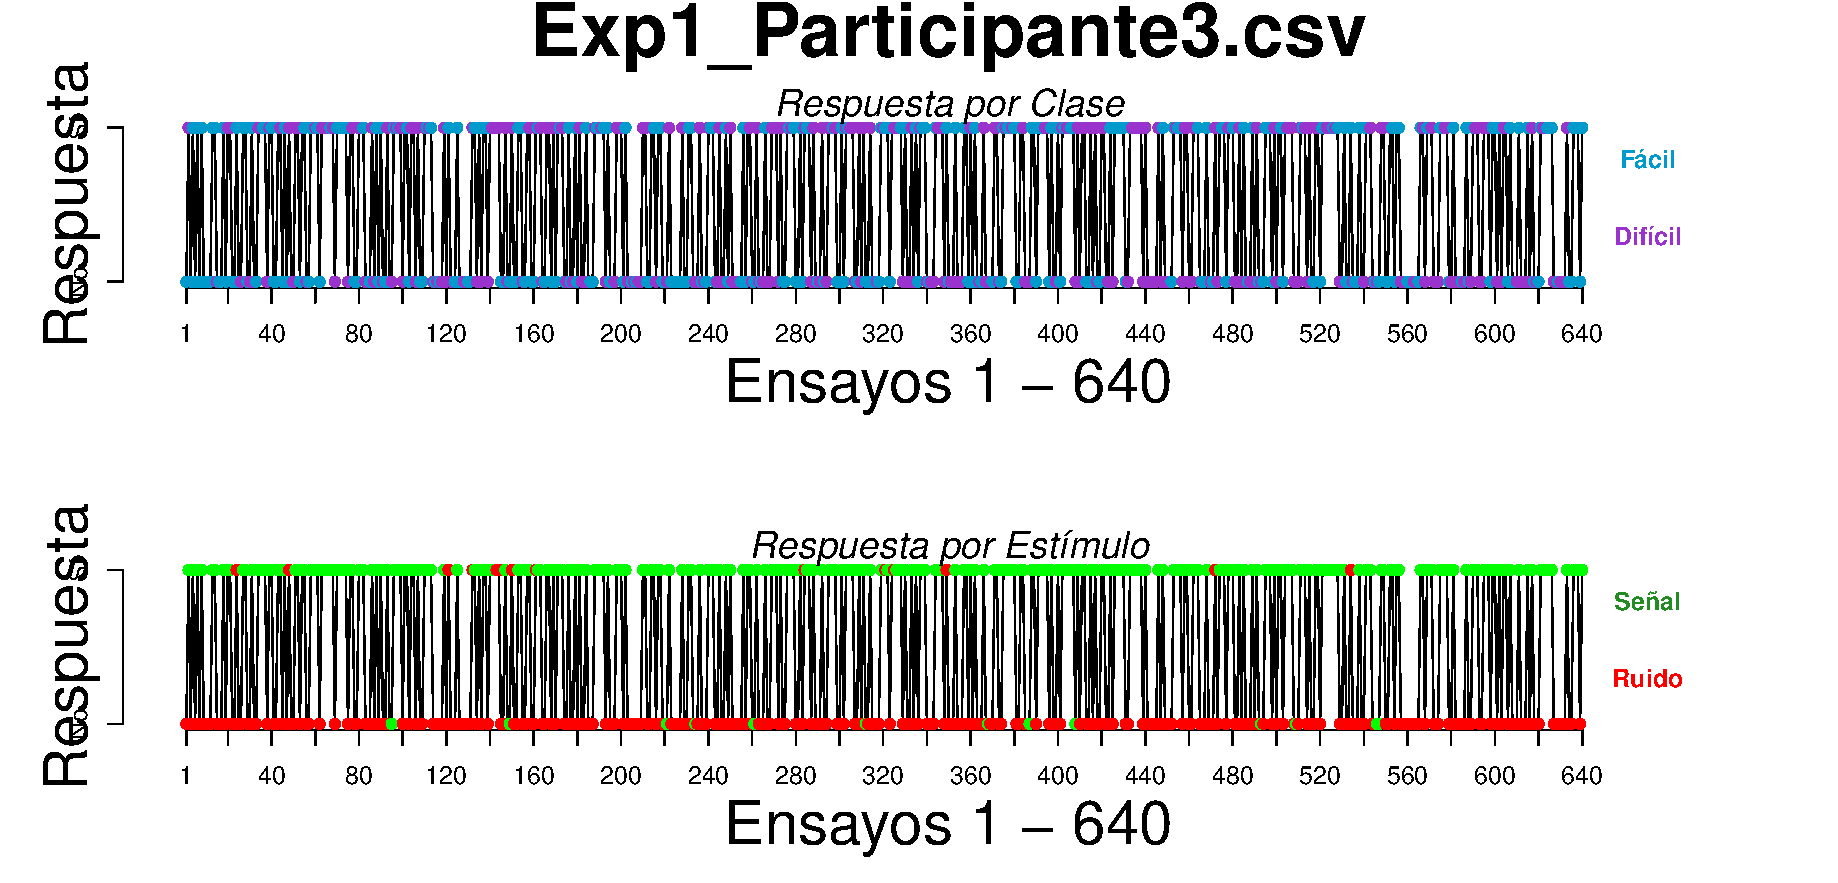
\includegraphics[width=9cm, height=5cm]{Figures/BiasResp_Exp1_P3} 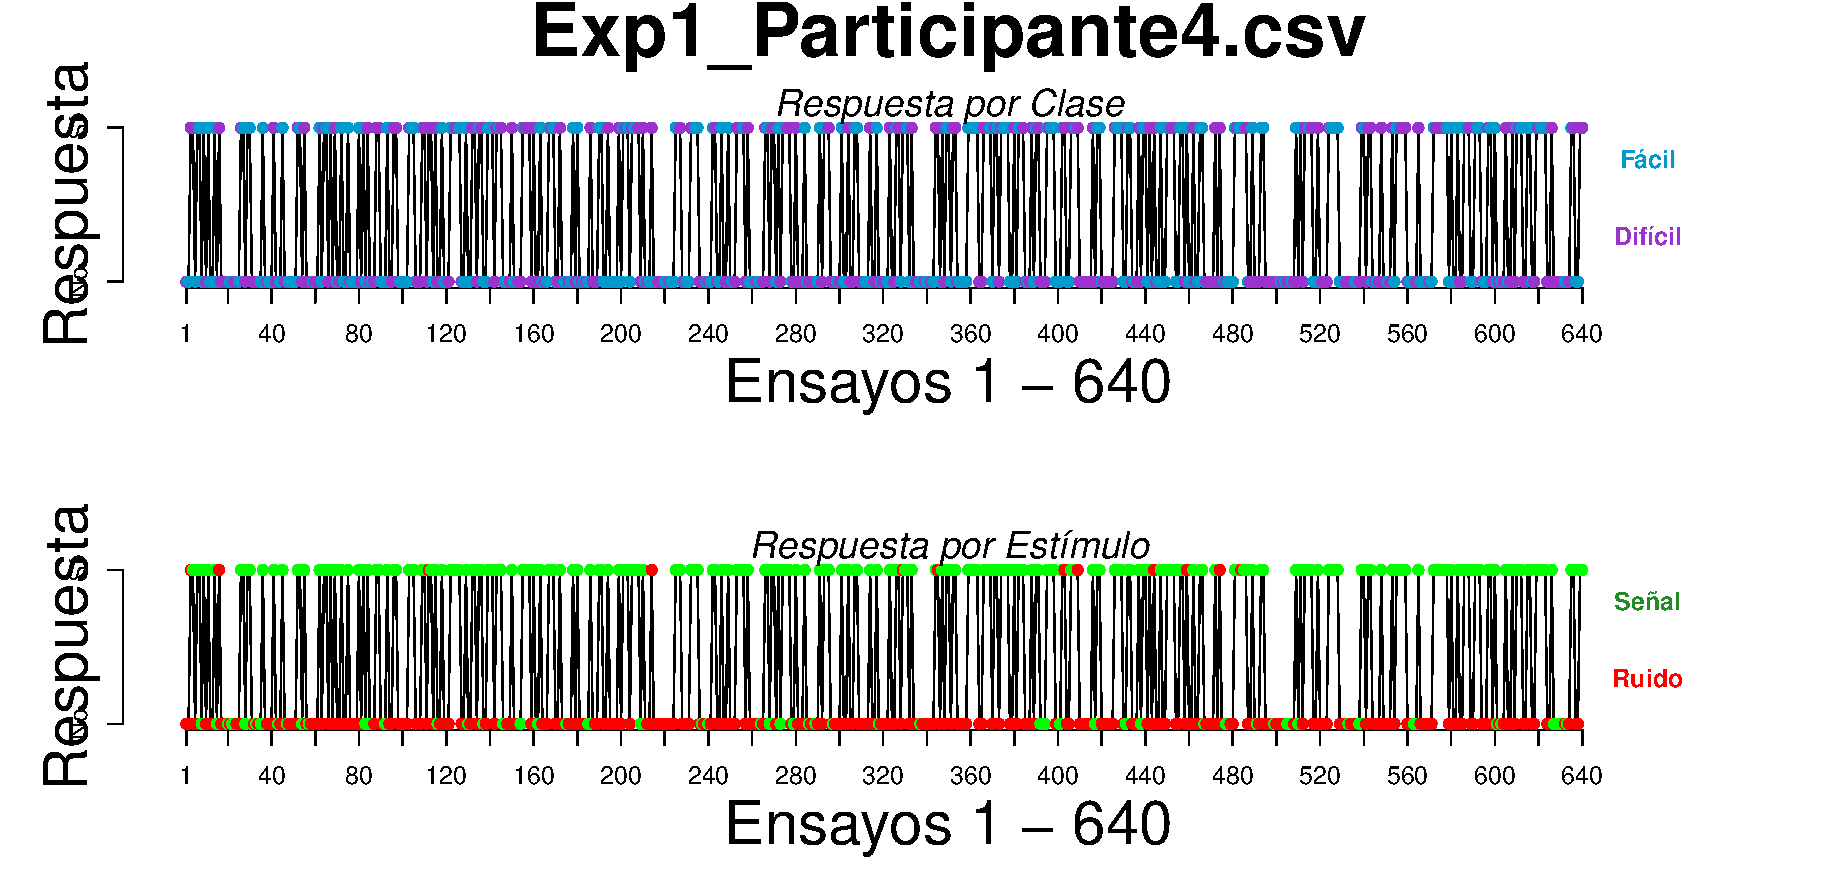
\includegraphics[width=9cm, height=5cm]{Figures/BiasResp_Exp1_P4} 
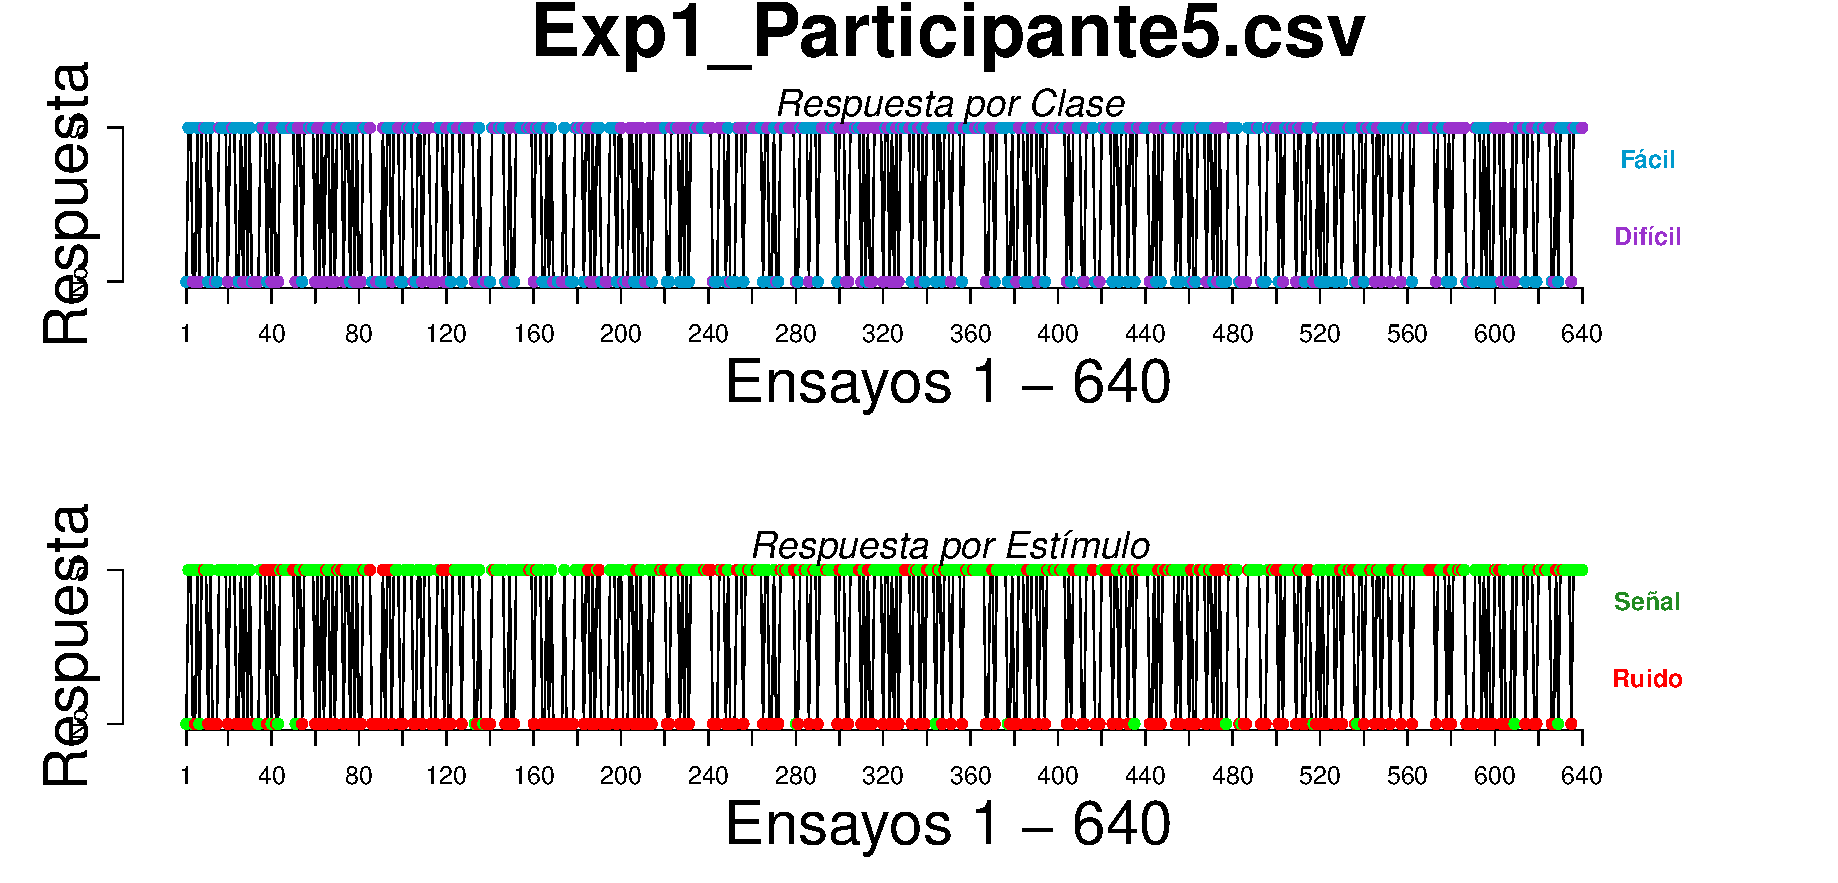
\includegraphics[width=9cm, height=5cm]{Figures/BiasResp_Exp1_P5} 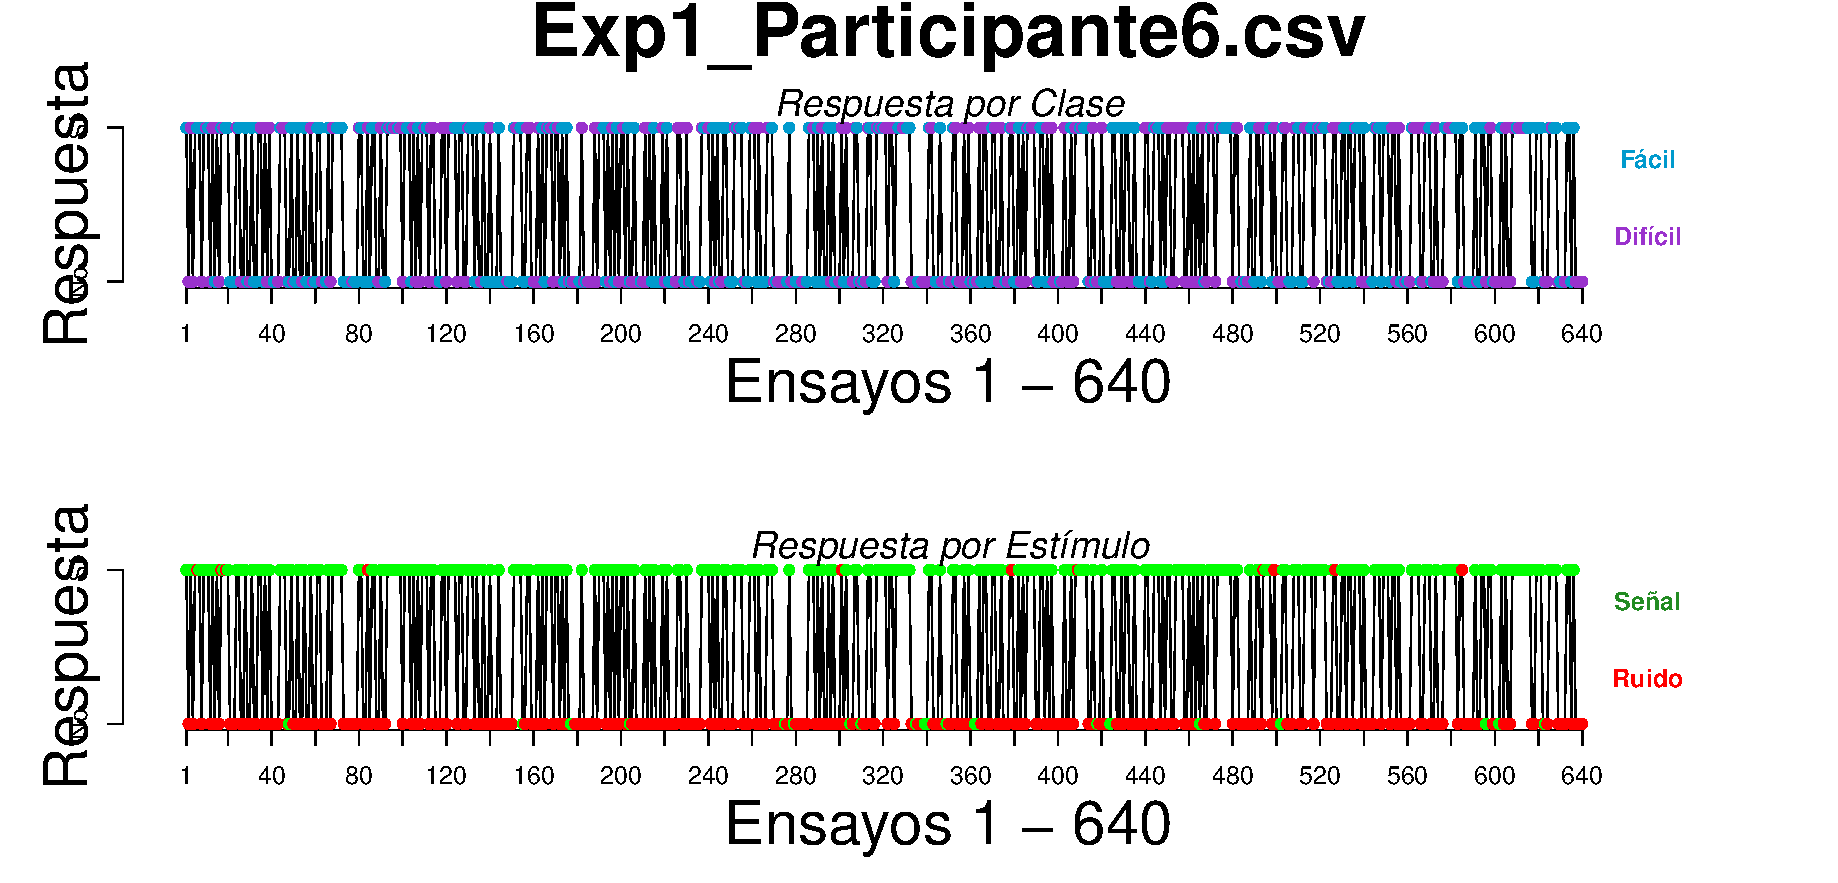
\includegraphics[width=9cm, height=5cm]{Figures/BiasResp_Exp1_P6}
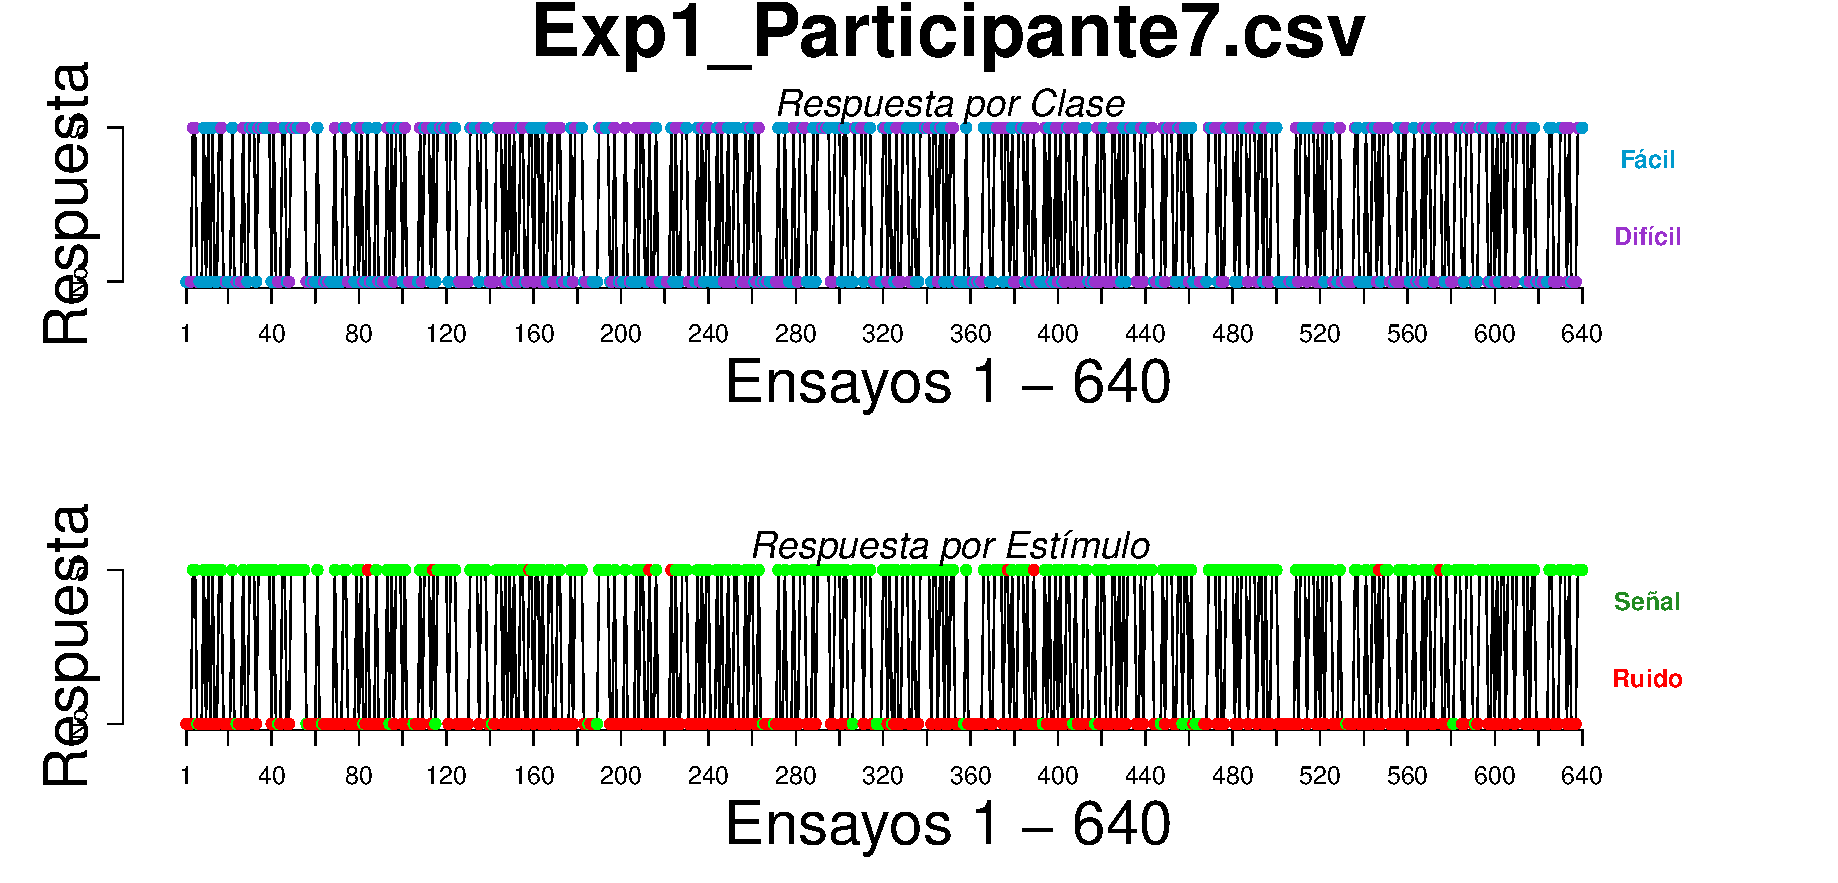
\includegraphics[width=9cm, height=5cm]{Figures/BiasResp_Exp1_P7} 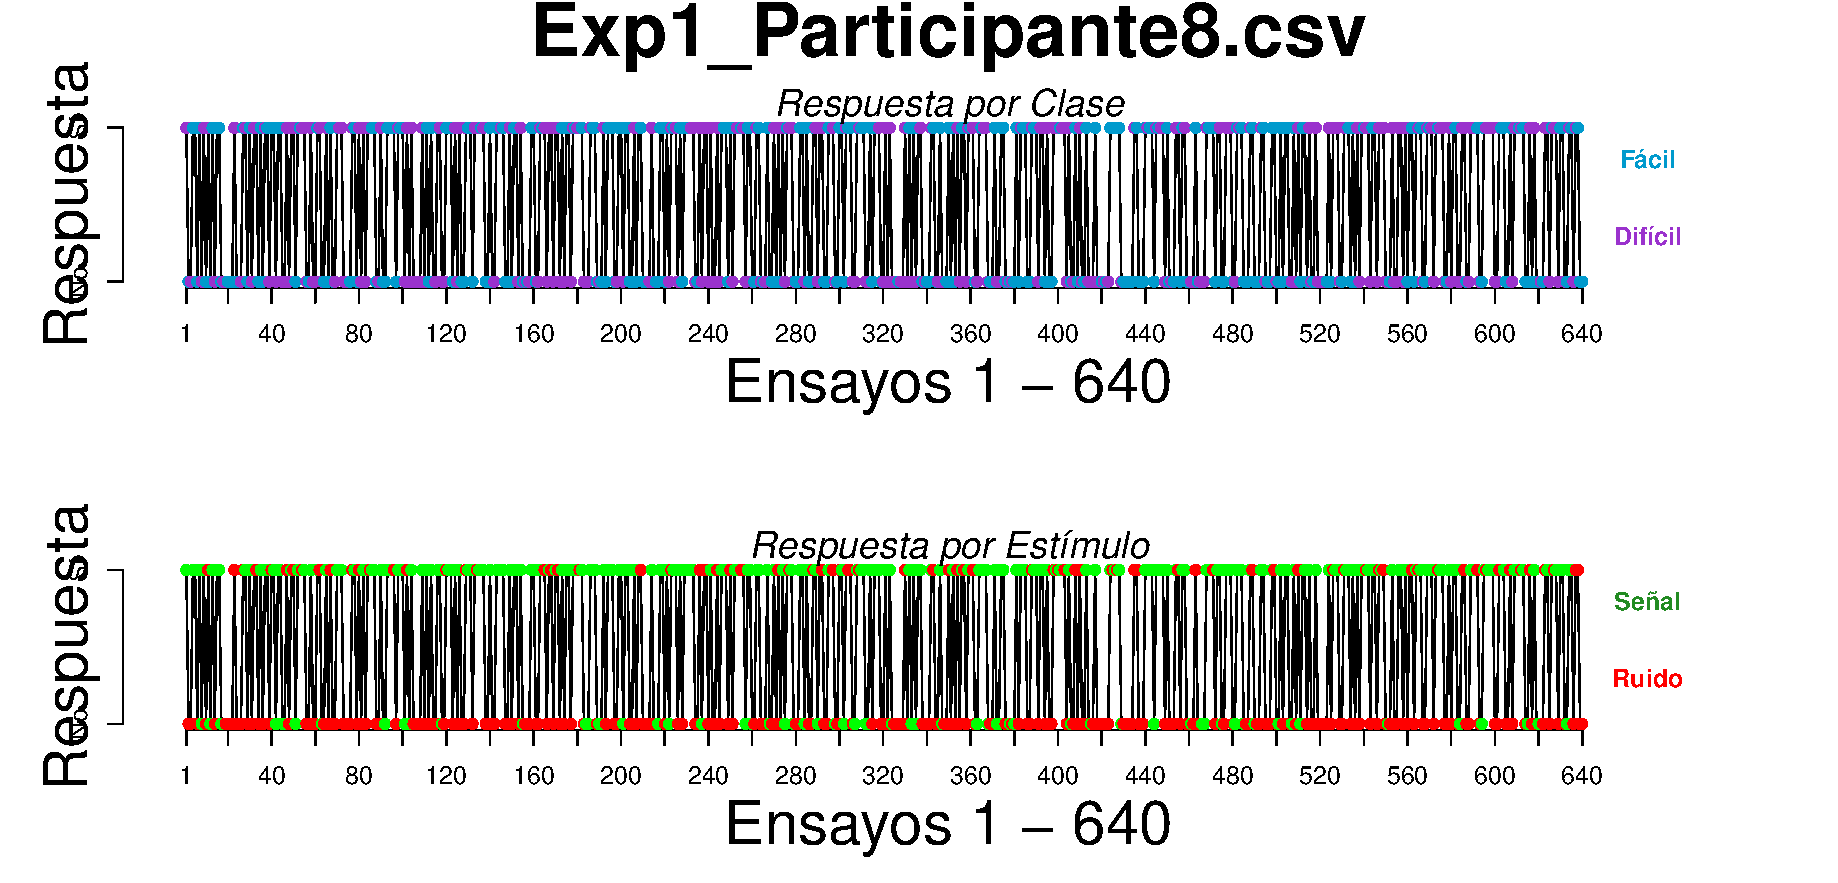
\includegraphics[width=9cm, height=5cm]{Figures/BiasResp_Exp1_P8} 
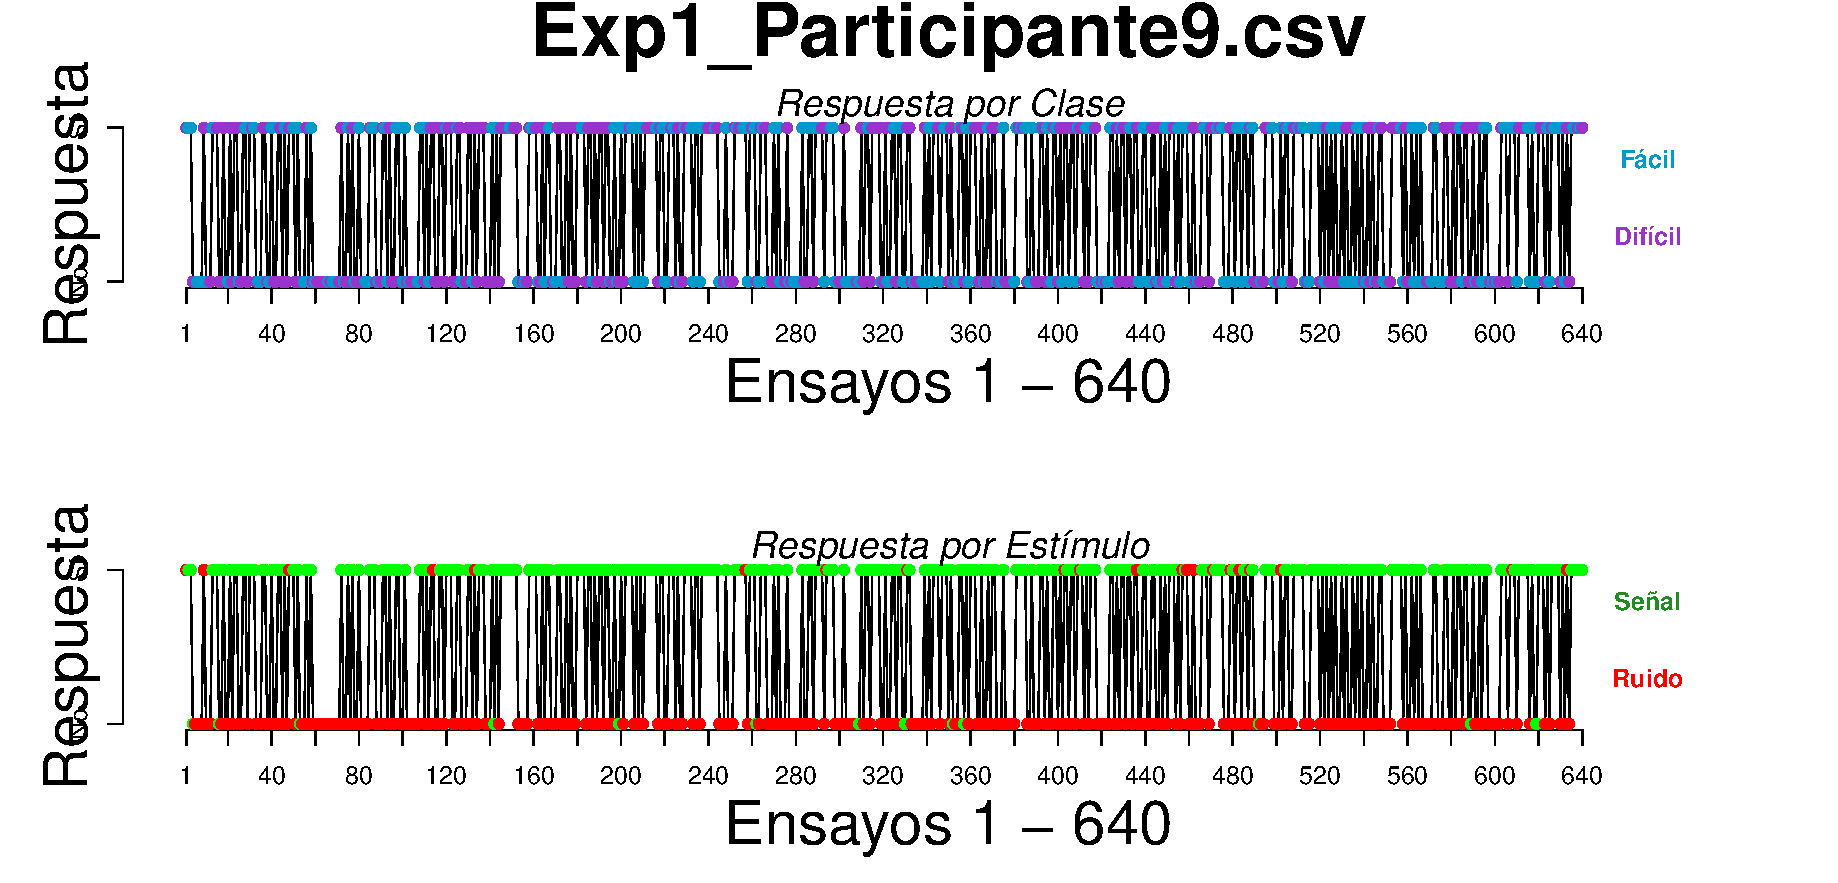
\includegraphics[width=9cm, height=5cm]{Figures/BiasResp_Exp1_P9}
\end{figure}
\vfill .
\begin{figure}[th]
\begin{center}
\includegraphics[width=8cm, height=4cm]{Figures/BiasResp_Exp1_P10} \includegraphics[width=8cm, height=4cm]{Figures/BiasResp_Exp1_P11} \includegraphics[width=8cm, height=4cm]{Figures/BiasResp_Exp1_P12}
\includegraphics[width=8cm, height=4cm]{Figures/BiasResp_Exp1_P13} \includegraphics[width=8cm, height=4cm]{Figures/BiasResp_Exp1_P14} \includegraphics[width=8cm, height=4cm]{Figures/BiasResp_Exp1_P15}
\includegraphics[width=8cm, height=4cm]{Figures/BiasResp_Exp1_P16} \includegraphics[width=8cm, height=4cm]{Figures/BiasResp_Exp1_P17} \includegraphics[width=8cm, height=4cm]{Figures/BiasResp_Exp1_P18}
\includegraphics[width=8cm, height=4cm]{Figures/BiasResp_Exp1_P19} \includegraphics[width=8cm, height=4cm]{Figures/BiasResp_Exp1_P20} \includegraphics[width=8cm, height=4cm]{Figures/BiasResp_Exp1_P21} 
\end{center}
\end{figure}
\clearpage



---
\vspace{3mm}
\begin{center}
{\LARGE \textbf{Correlación entre la Respuesta binaria registrada y el tipo de ensayo}}\\
{\small \textsc{(evaluando sesgos evidentes)}}\\
\smallskip
\end{center}
\begin{center}
{\LARGE \textit{Experimento 2}}\\
\end{center}
\vspace{3mm}
\begin{figure}[th]
\centering
\includegraphics[width=9cm, height=5cm]{Figures/BiasResp_Exp2_P1} \includegraphics[width=9cm, height=5cm]{Figures/BiasResp_Exp2_P2} 
\includegraphics[width=9cm, height=5cm]{Figures/BiasResp_Exp2_P3} \includegraphics[width=9cm, height=5cm]{Figures/BiasResp_Exp2_P4} 
\includegraphics[width=9cm, height=5cm]{Figures/BiasResp_Exp2_P5} \includegraphics[width=9cm, height=5cm]{Figures/BiasResp_Exp2_P6}
\includegraphics[width=9cm, height=5cm]{Figures/BiasResp_Exp2_P7} \includegraphics[width=9cm, height=5cm]{Figures/BiasResp_Exp2_P8} 
\includegraphics[width=9cm, height=5cm]{Figures/BiasResp_Exp2_P9}
\end{figure}
\vfill .
\begin{figure}[th]
\begin{center}
\includegraphics[width=8cm, height=4cm]{Figures/BiasResp_Exp2_P10} \includegraphics[width=8cm, height=4cm]{Figures/BiasResp_Exp2_P11} \includegraphics[width=8cm, height=4cm]{Figures/BiasResp_Exp2_P12}
\includegraphics[width=8cm, height=4cm]{Figures/BiasResp_Exp2_P13} \includegraphics[width=8cm, height=4cm]{Figures/BiasResp_Exp2_P14} \includegraphics[width=8cm, height=4cm]{Figures/BiasResp_Exp2_P15}
\includegraphics[width=8cm, height=4cm]{Figures/BiasResp_Exp2_P16} \includegraphics[width=8cm, height=4cm]{Figures/BiasResp_Exp2_P17} \includegraphics[width=8cm, height=4cm]{Figures/BiasResp_Exp2_P18}
\includegraphics[width=8cm, height=4cm]{Figures/BiasResp_Exp2_P19} \includegraphics[width=8cm, height=4cm]{Figures/BiasResp_Exp2_P20} \includegraphics[width=8cm, height=4cm]{Figures/BiasResp_Exp2_P21} 
\end{center}
\end{figure}
\clearpage









---
\vspace{3mm}
\begin{center}
{\LARGE \textbf{Puntajes de Confianza registrados por ensayo}}\\
{\small \textsc{(Verificando que se usaran todas las opciones de respuesta)}}\\
\smallskip
\end{center}
\begin{center}
{\LARGE \textit{Experimento 1}}\\
\end{center}
\vspace{3mm}
\begin{figure}[th]
\centering
\includegraphics[width=9cm, height=5cm]{Figures/Rating_Exp1_P1} \includegraphics[width=9cm, height=5cm]{Figures/Rating_Exp1_P2} 
\includegraphics[width=9cm, height=5cm]{Figures/Rating_Exp1_P3} \includegraphics[width=9cm, height=5cm]{Figures/Rating_Exp1_P4} 
\includegraphics[width=9cm, height=5cm]{Figures/Rating_Exp1_P5} \includegraphics[width=9cm, height=5cm]{Figures/Rating_Exp1_P6}
\includegraphics[width=9cm, height=5cm]{Figures/Rating_Exp1_P7} \includegraphics[width=9cm, height=5cm]{Figures/Rating_Exp1_P8} 
\includegraphics[width=9cm, height=5cm]{Figures/Rating_Exp1_P9}
\end{figure}
\vfill .
\begin{figure}[th]
\begin{center}
\includegraphics[width=8cm, height=4cm]{Figures/Rating_Exp1_P10} \includegraphics[width=8cm, height=4cm]{Figures/Rating_Exp1_P11} \includegraphics[width=8cm, height=4cm]{Figures/Rating_Exp1_P12}
\includegraphics[width=8cm, height=4cm]{Figures/Rating_Exp1_P13} \includegraphics[width=8cm, height=4cm]{Figures/Rating_Exp1_P14} \includegraphics[width=8cm, height=4cm]{Figures/Rating_Exp1_P15}
\includegraphics[width=8cm, height=4cm]{Figures/Rating_Exp1_P16} \includegraphics[width=8cm, height=4cm]{Figures/Rating_Exp1_P17} \includegraphics[width=8cm, height=4cm]{Figures/Rating_Exp1_P18}
\includegraphics[width=8cm, height=4cm]{Figures/Rating_Exp1_P19} \includegraphics[width=8cm, height=4cm]{Figures/Rating_Exp1_P20} 
\end{center}
\end{figure}
\clearpage



---
\vspace{3mm}
\begin{center}
{\LARGE \textbf{Puntajes de Confianza registrados por ensayo}}\\
{\small \textsc{(Verificando que se usaran todas las opciones de respuesta)}}\\
\smallskip
\end{center}
\begin{center}
{\LARGE \textit{Experimento 2}}\\
\end{center}
\vspace{3mm}
\begin{figure}[th]
\centering
\includegraphics[width=9cm, height=5cm]{Figures/Rating_Exp2_P1} \includegraphics[width=9cm, height=5cm]{Figures/Rating_Exp2_P2} 
\includegraphics[width=9cm, height=5cm]{Figures/Rating_Exp2_P3} \includegraphics[width=9cm, height=5cm]{Figures/Rating_Exp2_P4} 
\includegraphics[width=9cm, height=5cm]{Figures/Rating_Exp2_P5} \includegraphics[width=9cm, height=5cm]{Figures/Rating_Exp2_P6}
\includegraphics[width=9cm, height=5cm]{Figures/Rating_Exp2_P7} \includegraphics[width=9cm, height=5cm]{Figures/Rating_Exp2_P8} 
\includegraphics[width=9cm, height=5cm]{Figures/Rating_Exp2_P9}
\end{figure}
\vfill .
\begin{figure}[th]
\begin{center}
\includegraphics[width=8cm, height=4cm]{Figures/Rating_Exp2_P10} \includegraphics[width=8cm, height=4cm]{Figures/Rating_Exp2_P11} \includegraphics[width=8cm, height=4cm]{Figures/Rating_Exp2_P12}
\includegraphics[width=8cm, height=4cm]{Figures/Rating_Exp2_P13} \includegraphics[width=8cm, height=4cm]{Figures/Rating_Exp2_P14} \includegraphics[width=8cm, height=4cm]{Figures/Rating_Exp2_P15}
\includegraphics[width=8cm, height=4cm]{Figures/Rating_Exp2_P16} \includegraphics[width=8cm, height=4cm]{Figures/Rating_Exp2_P17} \includegraphics[width=8cm, height=4cm]{Figures/Rating_Exp2_P18}
\includegraphics[width=8cm, height=4cm]{Figures/Rating_Exp2_P19} \includegraphics[width=8cm, height=4cm]{Figures/Rating_Exp2_P20} \includegraphics[width=8cm, height=4cm]{Figures/Rating_Exp2_P21}
\end{center}
\end{figure}
\clearpage











---
\vspace{3mm}
\begin{center}
{\LARGE \textbf{Aciertos y errores cometidos a lo largo del tiempo}}\\
{\small \textsc{(Evaluar cambios en el desempeño de los participantes dependientes del tiempo)}}\\
\smallskip
\end{center}
\begin{center}
{\LARGE \textit{Experimento 1}}\\
\end{center}
\vspace{3mm}
\begin{figure}[th]
\centering
\includegraphics[width=9cm, height=5cm]{Figures/Success_Exp1_P1} \includegraphics[width=9cm, height=5cm]{Figures/Success_Exp1_P2} 
\includegraphics[width=9cm, height=5cm]{Figures/Success_Exp1_P3} \includegraphics[width=9cm, height=5cm]{Figures/Success_Exp1_P4} 
\includegraphics[width=9cm, height=5cm]{Figures/Success_Exp1_P5} \includegraphics[width=9cm, height=5cm]{Figures/Success_Exp1_P6}
\includegraphics[width=9cm, height=5cm]{Figures/Success_Exp1_P7} \includegraphics[width=9cm, height=5cm]{Figures/Success_Exp1_P8} 
\includegraphics[width=9cm, height=5cm]{Figures/Success_Exp1_P9}
\end{figure}
\vfill .
\begin{figure}[th]
\begin{center}
\includegraphics[width=8cm, height=4cm]{Figures/Success_Exp1_P10} \includegraphics[width=8cm, height=4cm]{Figures/Success_Exp1_P11} \includegraphics[width=8cm, height=4cm]{Figures/Success_Exp1_P12}
\includegraphics[width=8cm, height=4cm]{Figures/Success_Exp1_P13} \includegraphics[width=8cm, height=4cm]{Figures/Success_Exp1_P14} \includegraphics[width=8cm, height=4cm]{Figures/Success_Exp1_P15}
\includegraphics[width=8cm, height=4cm]{Figures/Success_Exp1_P16} \includegraphics[width=8cm, height=4cm]{Figures/Success_Exp1_P17} \includegraphics[width=8cm, height=4cm]{Figures/Success_Exp1_P18}
\includegraphics[width=8cm, height=4cm]{Figures/Success_Exp1_P19} \includegraphics[width=8cm, height=4cm]{Figures/Success_Exp1_P20} 
\end{center}
\end{figure}
\clearpage



---
\vspace{3mm}
\begin{center}
{\LARGE \textbf{Aciertos y errores cometidos a lo largo del tiempo}}\\
{\small \textsc{(Evaluar cambios en el desempeño de los participantes dependientes del tiempo)}}\\
\smallskip
\end{center}
\begin{center}
{\LARGE \textit{Experimento 2}}\\
\end{center}
\vspace{3mm}
\begin{figure}[th]
\centering
\includegraphics[width=9cm, height=5cm]{Figures/Success_Exp2_P1} \includegraphics[width=9cm, height=5cm]{Figures/Success_Exp2_P2} 
\includegraphics[width=9cm, height=5cm]{Figures/Success_Exp2_P3} \includegraphics[width=9cm, height=5cm]{Figures/Success_Exp2_P4} 
\includegraphics[width=9cm, height=5cm]{Figures/Success_Exp2_P5} \includegraphics[width=9cm, height=5cm]{Figures/Success_Exp2_P6}
\includegraphics[width=9cm, height=5cm]{Figures/Success_Exp2_P7} \includegraphics[width=9cm, height=5cm]{Figures/Success_Exp2_P8} 
\includegraphics[width=9cm, height=5cm]{Figures/Success_Exp2_P9}
\end{figure}
\vfill .
\begin{figure}[th]
\begin{center}
\includegraphics[width=8cm, height=4cm]{Figures/Success_Exp2_P10} \includegraphics[width=8cm, height=4cm]{Figures/Success_Exp2_P11} \includegraphics[width=8cm, height=4cm]{Figures/Success_Exp2_P12}
\includegraphics[width=8cm, height=4cm]{Figures/Success_Exp2_P13} \includegraphics[width=8cm, height=4cm]{Figures/Success_Exp2_P14} \includegraphics[width=8cm, height=4cm]{Figures/Success_Exp2_P15}
\includegraphics[width=8cm, height=4cm]{Figures/Success_Exp2_P16} \includegraphics[width=8cm, height=4cm]{Figures/Success_Exp2_P17} \includegraphics[width=8cm, height=4cm]{Figures/Success_Exp2_P18}
\includegraphics[width=8cm, height=4cm]{Figures/Success_Exp2_P19} \includegraphics[width=8cm, height=4cm]{Figures/Success_Exp2_P20} \includegraphics[width=8cm, height=4cm]{Figures/Success_Exp2_P21} 
\end{center}
\end{figure}
\clearpage
















---
\vspace{3mm}
\begin{center}
{\LARGE \textbf{Resultado obtenido en cada ensayo}}\\
{\small \textsc{(Evaluar cambios en el desempeño de los participantes dependientes del tiempo)}}\\
\smallskip
\end{center}
\begin{center}
{\LARGE \textit{Experimento 1}}\\
\end{center}
\vspace{3mm}
\begin{figure}[th]
\centering
\includegraphics[width=9cm, height=5cm]{Figures/Outcome_Exp1_P1} \includegraphics[width=9cm, height=5cm]{Figures/Outcome_Exp1_P2} 
\includegraphics[width=9cm, height=5cm]{Figures/Outcome_Exp1_P3} \includegraphics[width=9cm, height=5cm]{Figures/Outcome_Exp1_P4} 
\includegraphics[width=9cm, height=5cm]{Figures/Outcome_Exp1_P5} \includegraphics[width=9cm, height=5cm]{Figures/Outcome_Exp1_P6}
\includegraphics[width=9cm, height=5cm]{Figures/Outcome_Exp1_P7} \includegraphics[width=9cm, height=5cm]{Figures/Outcome_Exp1_P8} 
\includegraphics[width=9cm, height=5cm]{Figures/Outcome_Exp1_P9}
\end{figure}
\vfill .
\begin{figure}[th]
\begin{center}
\includegraphics[width=8cm, height=4cm]{Figures/Outcome_Exp1_P10} \includegraphics[width=8cm, height=4cm]{Figures/Outcome_Exp1_P11} \includegraphics[width=8cm, height=4cm]{Figures/Outcome_Exp1_P12}
\includegraphics[width=8cm, height=4cm]{Figures/Outcome_Exp1_P13} \includegraphics[width=8cm, height=4cm]{Figures/Outcome_Exp1_P14} \includegraphics[width=8cm, height=4cm]{Figures/Outcome_Exp1_P15}
\includegraphics[width=8cm, height=4cm]{Figures/Outcome_Exp1_P16} \includegraphics[width=8cm, height=4cm]{Figures/Outcome_Exp1_P17} \includegraphics[width=8cm, height=4cm]{Figures/Outcome_Exp1_P18}
\includegraphics[width=8cm, height=4cm]{Figures/Outcome_Exp1_P19} \includegraphics[width=8cm, height=4cm]{Figures/Outcome_Exp1_P20} 
\end{center}
\end{figure}
\clearpage



---
\vspace{3mm}
\begin{center}
{\LARGE \textbf{Resultado obtenido en cada ensayo}}\\
{\small \textsc{(Evaluar cambios en el desempeño de los participantes dependientes del tiempo)}}\\
\smallskip
\end{center}
\begin{center}
{\LARGE \textit{Experimento 2}}\\
\end{center}
\vspace{3mm}
\begin{figure}[th]
\centering
\includegraphics[width=9cm, height=5cm]{Figures/Outcome_Exp2_P1} \includegraphics[width=9cm, height=5cm]{Figures/Outcome_Exp2_P2} 
\includegraphics[width=9cm, height=5cm]{Figures/Outcome_Exp2_P3} \includegraphics[width=9cm, height=5cm]{Figures/Outcome_Exp2_P4} 
\includegraphics[width=9cm, height=5cm]{Figures/Outcome_Exp2_P5} \includegraphics[width=9cm, height=5cm]{Figures/Outcome_Exp2_P6}
\includegraphics[width=9cm, height=5cm]{Figures/Outcome_Exp2_P7} \includegraphics[width=9cm, height=5cm]{Figures/Outcome_Exp2_P8} 
\includegraphics[width=9cm, height=5cm]{Figures/Outcome_Exp2_P9}
\end{figure}
\vfill .
\begin{figure}[th]
\begin{center}
\includegraphics[width=8cm, height=4cm]{Figures/Outcome_Exp2_P10} \includegraphics[width=8cm, height=4cm]{Figures/Outcome_Exp2_P11} \includegraphics[width=8cm, height=4cm]{Figures/Outcome_Exp2_P12}
\includegraphics[width=8cm, height=4cm]{Figures/Outcome_Exp2_P13} \includegraphics[width=8cm, height=4cm]{Figures/Outcome_Exp2_P14} \includegraphics[width=8cm, height=4cm]{Figures/Outcome_Exp2_P15}
\includegraphics[width=8cm, height=4cm]{Figures/Outcome_Exp2_P16} \includegraphics[width=8cm, height=4cm]{Figures/Outcome_Exp2_P17} \includegraphics[width=8cm, height=4cm]{Figures/Outcome_Exp2_P18}
\includegraphics[width=8cm, height=4cm]{Figures/Outcome_Exp2_P19} \includegraphics[width=8cm, height=4cm]{Figures/Outcome_Exp2_P20} \includegraphics[width=8cm, height=4cm]{Figures/Outcome_Exp2_P21}
\end{center}
\end{figure}
\clearpage
















---
\vspace{3mm}
\begin{center}
{\LARGE \textbf{Explorando correlación Color - Desempeño}}\\
{\small \textsc{(Descartando que el color de las figuras tenga un impacto en la ejecución)}}\\
\smallskip
\end{center}
\begin{center}
{\LARGE \textit{Experimento 1}}\\
\end{center}
\vspace{3mm}
\begin{figure}[th]
\centering
\includegraphics[width=9cm, height=5cm]{Figures/Color_Exp1_P1} \includegraphics[width=9cm, height=5cm]{Figures/Color_Exp1_P2} 
\includegraphics[width=9cm, height=5cm]{Figures/Color_Exp1_P3} \includegraphics[width=9cm, height=5cm]{Figures/Color_Exp1_P4} 
\includegraphics[width=9cm, height=5cm]{Figures/Color_Exp1_P5} \includegraphics[width=9cm, height=5cm]{Figures/Color_Exp1_P6}
\includegraphics[width=9cm, height=5cm]{Figures/Color_Exp1_P7} \includegraphics[width=9cm, height=5cm]{Figures/Color_Exp1_P8} 
\includegraphics[width=9cm, height=5cm]{Figures/Color_Exp1_P9}
\end{figure}
\vfill .
\begin{figure}[th]
\begin{center}
\includegraphics[width=8cm, height=4cm]{Figures/Color_Exp1_P10} \includegraphics[width=8cm, height=4cm]{Figures/Color_Exp1_P11} \includegraphics[width=8cm, height=4cm]{Figures/Color_Exp1_P12}
\includegraphics[width=8cm, height=4cm]{Figures/Color_Exp1_P13} \includegraphics[width=8cm, height=4cm]{Figures/Color_Exp1_P14} \includegraphics[width=8cm, height=4cm]{Figures/Color_Exp1_P15}
\includegraphics[width=8cm, height=4cm]{Figures/Color_Exp1_P16} \includegraphics[width=8cm, height=4cm]{Figures/Color_Exp1_P17} \includegraphics[width=8cm, height=4cm]{Figures/Color_Exp1_P18}
\includegraphics[width=8cm, height=4cm]{Figures/Color_Exp1_P19} \includegraphics[width=8cm, height=4cm]{Figures/Color_Exp1_P20} 
\end{center}
\end{figure}
\clearpage



\begin{center}
{\LARGE \textbf{Explorando correlación Color - Desempeño}}\\
{\small \textsc{(Descartando que el color de las figuras tenga un impacto en la ejecución)}}\\
\smallskip
\end{center}
\begin{center}
{\LARGE \textit{Experimento 2}}\\
\end{center}
\vspace{3mm}
\begin{figure}[th]
\centering
\includegraphics[width=9cm, height=5cm]{Figures/Color_Exp2_P1} \includegraphics[width=9cm, height=5cm]{Figures/Color_Exp2_P2} 
\includegraphics[width=9cm, height=5cm]{Figures/Color_Exp2_P3} \includegraphics[width=9cm, height=5cm]{Figures/Color_Exp2_P4} 
\includegraphics[width=9cm, height=5cm]{Figures/Color_Exp2_P5} \includegraphics[width=9cm, height=5cm]{Figures/Color_Exp2_P6}
\includegraphics[width=9cm, height=5cm]{Figures/Color_Exp2_P7} \includegraphics[width=9cm, height=5cm]{Figures/Color_Exp2_P8} 
\includegraphics[width=9cm, height=5cm]{Figures/Color_Exp2_P9}
\end{figure}
\vfill .
\begin{figure}[th]
\begin{center}
\includegraphics[width=8cm, height=4cm]{Figures/Color_Exp2_P10} \includegraphics[width=8cm, height=4cm]{Figures/Color_Exp2_P11} \includegraphics[width=8cm, height=4cm]{Figures/Color_Exp2_P12}
\includegraphics[width=8cm, height=4cm]{Figures/Color_Exp2_P13} \includegraphics[width=8cm, height=4cm]{Figures/Color_Exp2_P14} \includegraphics[width=8cm, height=4cm]{Figures/Color_Exp2_P15}
\includegraphics[width=8cm, height=4cm]{Figures/Color_Exp2_P16} \includegraphics[width=8cm, height=4cm]{Figures/Color_Exp2_P17} \includegraphics[width=8cm, height=4cm]{Figures/Color_Exp2_P18}
\includegraphics[width=8cm, height=4cm]{Figures/Color_Exp2_P19} \includegraphics[width=8cm, height=4cm]{Figures/Color_Exp2_P20} \includegraphics[width=8cm, height=4cm]{Figures/Color_Exp2_P20} 
\end{center}
\end{figure}
\clearpage

















---
\vspace{3mm}
\begin{center}
{\LARGE \textbf{Evaluando relación Color - Sesgo a responder Sí/No}}\\
{\small \textsc{(Descartando que el color tenga un efecto en las respuestas emitidas)}}\\
\smallskip
\end{center}
\begin{center}
{\LARGE \textit{Experimento 1}}\\
\end{center}
\vspace{3mm}
\begin{figure}[th]
\centering
\includegraphics[width=9cm, height=5cm]{Figures/BiasColor_Exp1_P1} \includegraphics[width=9cm, height=5cm]{Figures/BiasColor_Exp1_P2} 
\includegraphics[width=9cm, height=5cm]{Figures/BiasColor_Exp1_P3} \includegraphics[width=9cm, height=5cm]{Figures/BiasColor_Exp1_P4} 
\includegraphics[width=9cm, height=5cm]{Figures/BiasColor_Exp1_P5} \includegraphics[width=9cm, height=5cm]{Figures/BiasColor_Exp1_P6}
\includegraphics[width=9cm, height=5cm]{Figures/BiasColor_Exp1_P7} \includegraphics[width=9cm, height=5cm]{Figures/BiasColor_Exp1_P8} 
\includegraphics[width=9cm, height=5cm]{Figures/BiasColor_Exp1_P9}
\end{figure}
\vfill .
\begin{figure}[th]
\begin{center}
\includegraphics[width=8cm, height=4cm]{Figures/BiasColor_Exp1_P10} \includegraphics[width=8cm, height=4cm]{Figures/BiasColor_Exp1_P11} \includegraphics[width=8cm, height=4cm]{Figures/BiasColor_Exp1_P12}
\includegraphics[width=8cm, height=4cm]{Figures/BiasColor_Exp1_P13} \includegraphics[width=8cm, height=4cm]{Figures/BiasColor_Exp1_P14} \includegraphics[width=8cm, height=4cm]{Figures/BiasColor_Exp1_P15}
\includegraphics[width=8cm, height=4cm]{Figures/BiasColor_Exp1_P16} \includegraphics[width=8cm, height=4cm]{Figures/BiasColor_Exp1_P17} \includegraphics[width=8cm, height=4cm]{Figures/BiasColor_Exp1_P18}
\includegraphics[width=8cm, height=4cm]{Figures/BiasColor_Exp1_P19} \includegraphics[width=8cm, height=4cm]{Figures/BiasColor_Exp1_P20} 
\end{center}
\end{figure}
\clearpage



\begin{center}
{\LARGE \textbf{Evaluando relación Color - Sesgo a responder Sí/No}}\\
{\small \textsc{(Descartando que el color tenga un efecto sobre las respuestas emitidas)}}\\
\smallskip
\end{center}
\begin{center}
{\LARGE \textit{Experimento 2}}\\
\end{center}
\vspace{3mm}
\begin{figure}[th]
\centering
\includegraphics[width=9cm, height=5cm]{Figures/BiasColor_Exp2_P1} \includegraphics[width=9cm, height=5cm]{Figures/BiasColor_Exp2_P2} 
\includegraphics[width=9cm, height=5cm]{Figures/BiasColor_Exp2_P3} \includegraphics[width=9cm, height=5cm]{Figures/BiasColor_Exp2_P4} 
\includegraphics[width=9cm, height=5cm]{Figures/BiasColor_Exp2_P5} \includegraphics[width=9cm, height=5cm]{Figures/BiasColor_Exp2_P6}
\includegraphics[width=9cm, height=5cm]{Figures/BiasColor_Exp2_P7} \includegraphics[width=9cm, height=5cm]{Figures/BiasColor_Exp2_P8} 
\includegraphics[width=9cm, height=5cm]{Figures/BiasColor_Exp2_P9}
\end{figure}
\vfill .
\begin{figure}[th]
\begin{center}
\includegraphics[width=8cm, height=4cm]{Figures/BiasColor_Exp2_P10} \includegraphics[width=8cm, height=4cm]{Figures/BiasColor_Exp2_P11} \includegraphics[width=8cm, height=4cm]{Figures/BiasColor_Exp2_P12}
\includegraphics[width=8cm, height=4cm]{Figures/BiasColor_Exp2_P13} \includegraphics[width=8cm, height=4cm]{Figures/BiasColor_Exp2_P14} \includegraphics[width=8cm, height=4cm]{Figures/BiasColor_Exp2_P15}
\includegraphics[width=8cm, height=4cm]{Figures/BiasColor_Exp2_P16} \includegraphics[width=8cm, height=4cm]{Figures/BiasColor_Exp2_P17} \includegraphics[width=8cm, height=4cm]{Figures/BiasColor_Exp2_P18}
\includegraphics[width=8cm, height=4cm]{Figures/BiasColor_Exp2_P19} \includegraphics[width=8cm, height=4cm]{Figures/BiasColor_Exp2_P20} \includegraphics[width=8cm, height=4cm]{Figures/BiasColor_Exp2_P21}
\end{center}
\end{figure}
\clearpage





















---
\vspace{3mm}
\begin{center}
{\LARGE \textbf{Evidencia del Efecto Espejo en la tarea binaria}}\\
{\small \textsc{(comprobando que FA(A)<FA(B)<H(B)>H(A))}}\\
\smallskip
\end{center}
\begin{center}
{\LARGE \textit{Experimento 1}}\\
\end{center}
\vspace{3mm}
\begin{figure}[th]
\centering
\includegraphics[width=9cm, height=5cm]{Figures/MirrorRate_Exp1_P1} \includegraphics[width=9cm, height=5cm]{Figures/MirrorRate_Exp1_P2} 
\includegraphics[width=9cm, height=5cm]{Figures/MirrorRate_Exp1_P3} \includegraphics[width=9cm, height=5cm]{Figures/MirrorRate_Exp1_P4} 
\includegraphics[width=9cm, height=5cm]{Figures/MirrorRate_Exp1_P5} \includegraphics[width=9cm, height=5cm]{Figures/MirrorRate_Exp1_P6}
\includegraphics[width=9cm, height=5cm]{Figures/MirrorRate_Exp1_P7} \includegraphics[width=9cm, height=5cm]{Figures/MirrorRate_Exp1_P8} 
\includegraphics[width=9cm, height=5cm]{Figures/MirrorRate_Exp1_P9}
\end{figure}
\vfill .
\begin{figure}[th]
\begin{center}
\includegraphics[width=8cm, height=4cm]{Figures/MirrorRate_Exp1_P10} \includegraphics[width=8cm, height=4cm]{Figures/MirrorRate_Exp1_P11} \includegraphics[width=8cm, height=4cm]{Figures/MirrorRate_Exp1_P12}
\includegraphics[width=8cm, height=4cm]{Figures/MirrorRate_Exp1_P13} \includegraphics[width=8cm, height=4cm]{Figures/MirrorRate_Exp1_P14} \includegraphics[width=8cm, height=4cm]{Figures/MirrorRate_Exp1_P15}
\includegraphics[width=8cm, height=4cm]{Figures/MirrorRate_Exp1_P16} \includegraphics[width=8cm, height=4cm]{Figures/MirrorRate_Exp1_P17} \includegraphics[width=8cm, height=4cm]{Figures/MirrorRate_Exp1_P18}
\includegraphics[width=8cm, height=4cm]{Figures/MirrorRate_Exp1_P19} \includegraphics[width=8cm, height=4cm]{Figures/MirrorRate_Exp1_P20} 
\end{center}
\end{figure}
\clearpage



\begin{center}
{\LARGE \textbf{Evidencia del Efecto Espejo en la tarea binaria}}\\
{\small \textsc{(comprobando que FA(A)<FA(B)<H(B)>H(A))}}\\
\smallskip
\end{center}
\begin{center}
{\LARGE \textit{Experimento 2}}\\
\end{center}
\vspace{3mm}
\begin{figure}[th]
\centering
\includegraphics[width=9cm, height=5cm]{Figures/MirrorRate_Exp2_P1} \includegraphics[width=9cm, height=5cm]{Figures/MirrorRate_Exp2_P2} 
\includegraphics[width=9cm, height=5cm]{Figures/MirrorRate_Exp2_P3} \includegraphics[width=9cm, height=5cm]{Figures/MirrorRate_Exp2_P4} 
\includegraphics[width=9cm, height=5cm]{Figures/MirrorRate_Exp2_P5} \includegraphics[width=9cm, height=5cm]{Figures/MirrorRate_Exp2_P6}
\includegraphics[width=9cm, height=5cm]{Figures/MirrorRate_Exp2_P7} \includegraphics[width=9cm, height=5cm]{Figures/MirrorRate_Exp2_P8} 
\includegraphics[width=9cm, height=5cm]{Figures/MirrorRate_Exp2_P9}
\end{figure}
\vfill .
\begin{figure}[th]
\begin{center}
\includegraphics[width=8cm, height=4cm]{Figures/MirrorRate_Exp2_P10} \includegraphics[width=8cm, height=4cm]{Figures/MirrorRate_Exp2_P11} \includegraphics[width=8cm, height=4cm]{Figures/MirrorRate_Exp2_P12}
\includegraphics[width=8cm, height=4cm]{Figures/MirrorRate_Exp2_P13} \includegraphics[width=8cm, height=4cm]{Figures/MirrorRate_Exp2_P14} \includegraphics[width=8cm, height=4cm]{Figures/MirrorRate_Exp2_P15}
\includegraphics[width=8cm, height=4cm]{Figures/MirrorRate_Exp2_P16} \includegraphics[width=8cm, height=4cm]{Figures/MirrorRate_Exp2_P17} \includegraphics[width=8cm, height=4cm]{Figures/MirrorRate_Exp2_P18}
\includegraphics[width=8cm, height=4cm]{Figures/MirrorRate_Exp2_P19} \includegraphics[width=8cm, height=4cm]{Figures/MirrorRate_Exp2_P20} \includegraphics[width=8cm, height=4cm]{Figures/MirrorRate_Exp2_P21}
\end{center}
\end{figure}
\clearpage

















---
\vspace{3mm}
\begin{center}
{\LARGE \textbf{Evidencia del Efecto Espejo en la Escala de Confianza}}\\
{\small \textsc{(comprobando que R(AN)<R(BN)<R(BS)>R(AS))}}\\
\smallskip
\end{center}
\begin{center}
{\LARGE \textit{Experimento 1}}\\
\end{center}
\vspace{3mm}
\begin{figure}[th]
\centering
\includegraphics[width=9cm, height=5cm]{Figures/MirrorRating_Exp1_P1} \includegraphics[width=9cm, height=5cm]{Figures/MirrorRating_Exp1_P2} 
\includegraphics[width=9cm, height=5cm]{Figures/MirrorRating_Exp1_P3} \includegraphics[width=9cm, height=5cm]{Figures/MirrorRating_Exp1_P4} 
\includegraphics[width=9cm, height=5cm]{Figures/MirrorRating_Exp1_P5} \includegraphics[width=9cm, height=5cm]{Figures/MirrorRating_Exp1_P6}
\includegraphics[width=9cm, height=5cm]{Figures/MirrorRating_Exp1_P7} \includegraphics[width=9cm, height=5cm]{Figures/MirrorRating_Exp1_P8} 
\includegraphics[width=9cm, height=5cm]{Figures/MirrorRating_Exp1_P9}
\end{figure}
\vfill .
\begin{figure}[th]
\begin{center}
\includegraphics[width=8cm, height=4cm]{Figures/MirrorRating_Exp1_P10} \includegraphics[width=8cm, height=4cm]{Figures/MirrorRating_Exp1_P11} \includegraphics[width=8cm, height=4cm]{Figures/MirrorRating_Exp1_P12}
\includegraphics[width=8cm, height=4cm]{Figures/MirrorRating_Exp1_P13} \includegraphics[width=8cm, height=4cm]{Figures/MirrorRating_Exp1_P14} \includegraphics[width=8cm, height=4cm]{Figures/MirrorRating_Exp1_P15}
\includegraphics[width=8cm, height=4cm]{Figures/MirrorRating_Exp1_P16} \includegraphics[width=8cm, height=4cm]{Figures/MirrorRating_Exp1_P17} \includegraphics[width=8cm, height=4cm]{Figures/MirrorRating_Exp1_P18}
\includegraphics[width=8cm, height=4cm]{Figures/MirrorRating_Exp1_P19} \includegraphics[width=8cm, height=4cm]{Figures/MirrorRating_Exp1_P20} 
\end{center}
\end{figure}
\clearpage



\begin{center}
{\LARGE \textbf{Evidencia del Efecto Espejo en la Escala de Confianza}}\\
{\small \textsc{(comprobando que R(AN)<R(BN)<R(BS)>R(AS))}}\\
\smallskip
\end{center}
\begin{center}
{\LARGE \textit{Experimento 2}}\\
\end{center}
\vspace{3mm}
\begin{figure}[th]
\centering
\includegraphics[width=9cm, height=5cm]{Figures/MirrorRating_Exp2_P1} \includegraphics[width=9cm, height=5cm]{Figures/MirrorRating_Exp2_P2} 
\includegraphics[width=9cm, height=5cm]{Figures/MirrorRating_Exp2_P3} \includegraphics[width=9cm, height=5cm]{Figures/MirrorRating_Exp2_P4} 
\includegraphics[width=9cm, height=5cm]{Figures/MirrorRating_Exp2_P5} \includegraphics[width=9cm, height=5cm]{Figures/MirrorRating_Exp2_P6}
\includegraphics[width=9cm, height=5cm]{Figures/MirrorRating_Exp2_P7} \includegraphics[width=9cm, height=5cm]{Figures/MirrorRating_Exp2_P8} 
\includegraphics[width=9cm, height=5cm]{Figures/MirrorRating_Exp2_P9}
\end{figure}
\vfill .
\begin{figure}[th]
\begin{center}
\includegraphics[width=8cm, height=4cm]{Figures/MirrorRating_Exp2_P10} \includegraphics[width=8cm, height=4cm]{Figures/MirrorRating_Exp2_P11} \includegraphics[width=8cm, height=4cm]{Figures/MirrorRating_Exp2_P12}
\includegraphics[width=8cm, height=4cm]{Figures/MirrorRating_Exp2_P13} \includegraphics[width=8cm, height=4cm]{Figures/MirrorRating_Exp2_P14} \includegraphics[width=8cm, height=4cm]{Figures/MirrorRating_Exp2_P15}
\includegraphics[width=8cm, height=4cm]{Figures/MirrorRating_Exp2_P16} \includegraphics[width=8cm, height=4cm]{Figures/MirrorRating_Exp2_P17} \includegraphics[width=8cm, height=4cm]{Figures/MirrorRating_Exp2_P18}
\includegraphics[width=8cm, height=4cm]{Figures/MirrorRating_Exp2_P19} \includegraphics[width=8cm, height=4cm]{Figures/MirrorRating_Exp2_P20} \includegraphics[width=8cm, height=4cm]{Figures/MirrorRating_Exp2_P21}
\end{center}
\end{figure}
\clearpage







\end{document}